% MAIN.TEX - File chính của báo cáo
% Hệ thống quản lý quy trình sản xuất Manga


\documentclass[a4paper, 12pt]{report}

% --- Nạp cấu hình ---
% ====================================
% PACKAGES - Khai báo các gói cần thiết
% ====================================

\PassOptionsToPackage{table,xcdraw}{xcolor}

% Ngôn ngữ và mã hóa
\usepackage[utf8]{inputenc}
\usepackage[vietnamese]{babel}
\usepackage[T5]{fontenc}
\usepackage{times}
\usepackage{courier}
\usepackage{indentfirst}
\usepackage[verbose=silent]{microtype}

% Toán học
\usepackage{amsmath, amssymb, amsfonts}

% Đồ họa và hình ảnh
\usepackage{graphicx}
\usepackage{float}
\usepackage{subcaption}
\usepackage{tikz}
\usetikzlibrary{positioning}
\usepackage{pdflscape}

% Bảng biểu
\usepackage{booktabs}
\usepackage{tabularx}
\usepackage{longtable}
\usepackage{multirow}
\usepackage{array}

% Định dạng trang
\usepackage[fontsize=13pt]{scrextend}
\usepackage{geometry}
\usepackage{setspace}
\usepackage{fancyhdr}
\usepackage{titlesec}
\usepackage{textcase}

% Mục lục
\usepackage[titles]{tocloft}

% Liên kết và tham chiếu
\usepackage{hyperref}
\usepackage{url}
\usepackage[nameinlink]{cleveref}

% Mã nguồn
\usepackage{listings}
\usepackage{xcolor}

% Danh sách và liệt kê
\usepackage{enumitem}

% Phụ lục
\usepackage{appendix}


% Caption
\usepackage{caption}

% Glossary / Thuật ngữ
\usepackage[acronym, toc]{glossaries}

\usepackage{placeins}
% ====================================
% FORMATTING - Định dạng tài liệu
% ====================================

% Định nghĩa bảng màu đen trắng (theo yêu cầu chữ màu đen)
\definecolor{navyblue}{RGB}{0, 0, 0}          % Đen cho tiêu đề, header
\definecolor{charcoal}{RGB}{0, 0, 0}          % Đen cho chữ chính
\definecolor{lightgray}{RGB}{245, 247, 250}   % Nền xám nhạt cho code
\definecolor{bordergray}{RGB}{220, 224, 230}  % Màu viền cho bảng/code
\definecolor{linkblue}{RGB}{0, 0, 0}          % Đen cho link
\definecolor{citegreen}{RGB}{0, 0, 0}         % Đen cho trích dẫn
\definecolor{tableheader}{RGB}{224, 235, 250} % Màu nền xanh xám nhạt cho header bảng

% Thiết lập lề trang
\geometry{
    a4paper,
    left=3cm,
    right=2cm,
    top=2.5cm,
    bottom=2.5cm
}

% Giãn dòng 1.5
\onehalfspacing

% Chiều cao header tránh cảnh báo lỗi
\setlength{\headheight}{15pt}

% Thiết lập header và footer
\pagestyle{fancy}
\fancyhf{}
\fancyhead[L]{\small\color{navyblue} Hệ thống quản lý quy trình sáng tác và xuất bản Manga}
\fancyhead[R]{\small\color{navyblue} Software Engineering}
\fancyfoot[C]{\small\color{navyblue}\thepage}
\renewcommand{\headrulewidth}{0.5pt}
\renewcommand{\headrule}{{\color{navyblue}\hrule width\headwidth height\headrulewidth\hfill}}
\renewcommand{\footrulewidth}{0pt}

% Định nghĩa viết hoa cho tên chương và phụ lục
\addto\captionsvietnamese{%
  \renewcommand{\chaptername}{CHƯƠNG}%
  \renewcommand{\appendixname}{PHỤ LỤC}%
}

% Định dạng tiêu đề chương trên 1 hàng, viết hoa toàn bộ
\titleformat{\chapter}[hang]
    {\normalfont\fontsize{16pt}{20pt}\selectfont\bfseries\color{navyblue}\centering}
    {\chaptertitlename~\thechapter.~}
    {0em}
    {\MakeTextUppercase}
\titlespacing*{\chapter}{0pt}{-10pt}{30pt}

% Định dạng tiêu đề mục
\titleformat{\section}
    {\normalfont\fontsize{14pt}{18pt}\selectfont\bfseries\color{navyblue}}
    {\thesection}{1em}{}
\titlespacing*{\section}{0pt}{18pt}{10pt}

\titleformat{\subsection}
    {\normalfont\fontsize{13pt}{16.5pt}\selectfont\bfseries\color{navyblue}}
    {\thesubsection}{1em}{}
\titlespacing*{\subsection}{0pt}{14pt}{6pt}

\titleformat{\subsubsection}
    {\normalfont\fontsize{12pt}{15pt}\selectfont\bfseries\color{navyblue}}
    {\thesubsubsection}{1em}{}
\titlespacing*{\subsubsection}{0pt}{10pt}{4pt}

% Độ sâu mục lục
\setcounter{tocdepth}{2}
\setcounter{secnumdepth}{3}

% Cấu hình hiển thị tiền tố "Hình" và "Bảng" trong Danh sách hình vẽ & Danh sách bảng
\renewcommand{\cftfigpresnum}{Hình~}
\renewcommand{\cftfigaftersnum}{:}
\setlength{\cftfignumwidth}{5.0em}

\renewcommand{\cfttabpresnum}{Bảng~}
\renewcommand{\cfttabaftersnum}{:}
\setlength{\cfttabnumwidth}{5.0em}

% Thiết lập hyperref
\hypersetup{
    colorlinks=true,
    linkcolor=linkblue,
    filecolor=magenta,
    urlcolor=linkblue,
    citecolor=citegreen,
    pdftitle={Báo cáo đồ án},
    pdfauthor={Tác giả},
    bookmarks=true
}

% Thiết lập listings cho mã nguồn
\lstset{
    backgroundcolor=\color{lightgray},
    basicstyle=\ttfamily\small\color{charcoal},
    breakatwhitespace=false,
    breaklines=true,
    captionpos=b,
    commentstyle=\color{citegreen}\itshape,
    frame=single,
    rulecolor=\color{bordergray},
    numbers=left,
    numberstyle=\tiny\color{black},
    keywordstyle=\color{navyblue}\bfseries,
    stringstyle=\color{black},
    showstringspaces=false,
    tabsize=4,
    keepspaces=true
}

% Thiết lập caption
\captionsetup{
    font=small,
    labelfont=bf,
    justification=centering
}

% Định dạng đường dẫn hình ảnh
\graphicspath{{assets/images/}{assets/diagrams/}}

% ====================================
% COMMANDS - Các lệnh tùy chỉnh
% ====================================

% Thông tin đồ án
\newcommand{\tentruong}{Trường Đại học ...}
\newcommand{\tenkhoa}{Khoa Công nghệ Thông tin}
\newcommand{\tendoan}{Hệ thống quản lý quy trình sản xuất Manga}
\newcommand{\tenmonhoc}{Lập trình Web}
\newcommand{\tensinhvien}{Họ và tên sinh viên}
\newcommand{\mssv}{MSSV}
\newcommand{\tengvhd}{Họ và tên giảng viên}
\newcommand{\namhoc}{2025 -- 2026}

% Lệnh tiện ích
\newcommand{\figref}[1]{Hình~\ref{#1}}
\newcommand{\tabref}[1]{Bảng~\ref{#1}}
\newcommand{\eqnref}[1]{Công thức~(\ref{#1})}
\newcommand{\chapref}[1]{Chương~\ref{#1}}
\newcommand{\secref}[1]{Mục~\ref{#1}}

% Lệnh cho code inline
\newcommand{\code}[1]{\texttt{#1}}

% Lệnh cho từ khóa kỹ thuật
\newcommand{\tech}[1]{\textit{#1}}

% Lệnh tạo dòng kẻ ngang
\newcommand{\HRule}{\rule{\linewidth}{0.5mm}}


% ====================================
% BẮT ĐẦU TÀI LIỆU
% ====================================
\begin{document}

\pagenumbering{alph} % Trang bìa là trang 'a' để tránh trùng lặp anchor page 1 với Chương 1

% --- Trang bìa ---
% ====================================
% TRANG BÌA
% ====================================

\begin{titlepage}
    % Thiết lập lề đối xứng cho trang bìa để căn giữa hoàn hảo
    \newgeometry{left=2.5cm, right=2.5cm, top=2cm, bottom=2cm}
    
    \begin{tikzpicture}[remember picture, overlay]
        % Định nghĩa màu đen cho khung viền
        \definecolor{navyblue}{RGB}{0, 0, 0}
        
        % Tọa độ cho khung viền ngoài đối xứng (cách đều các lề 2cm)
        \coordinate (TL) at ([shift={(2cm,-2cm)}]current page.north west);
        \coordinate (TR) at ([shift={(-2cm,-2cm)}]current page.north east);
        \coordinate (BL) at ([shift={(2cm,2cm)}]current page.south west);
        \coordinate (BR) at ([shift={(-2cm,2cm)}]current page.south east);
        
        \def\eps{4mm}  % Độ nhô ra của góc giao nhau
        \def\gap{2mm}  % Khoảng cách giữa 2 khung viền
        
        % Khung viền ngoài (nét mảnh 0.8pt)
        \draw[line width=0.8pt, navyblue] ([xshift=-\eps]TL) -- ([xshift=\eps]TR);
        \draw[line width=0.8pt, navyblue] ([xshift=-\eps]BL) -- ([xshift=\eps]BR);
        \draw[line width=0.8pt, navyblue] ([yshift=\eps]TL) -- ([yshift=-\eps]BL);
        \draw[line width=0.8pt, navyblue] ([yshift=\eps]TR) -- ([yshift=-\eps]BR);
        
        % Khung viền trong (nét dày 2.5pt)
        \coordinate (iTL) at ([shift={(\gap,-\gap)}]TL);
        \coordinate (iTR) at ([shift={(-\gap,-\gap)}]TR);
        \coordinate (iBL) at ([shift={(\gap,\gap)}]BL);
        \coordinate (iBR) at ([shift={(-\gap,\gap)}]BR);
        
        \draw[line width=2.5pt, navyblue] ([xshift=-\eps]iTL) -- ([xshift=\eps]iTR);
        \draw[line width=2.5pt, navyblue] ([xshift=-\eps]iBL) -- ([xshift=\eps]iBR);
        \draw[line width=2.5pt, navyblue] ([yshift=\eps]iTL) -- ([yshift=-\eps]iBL);
        \draw[line width=2.5pt, navyblue] ([yshift=\eps]iTR) -- ([yshift=-\eps]iBR);
    \end{tikzpicture}

    \begin{center}
        \vspace*{0.5cm}
        
        {\fontsize{18pt}{24pt}\selectfont \bfseries TRƯỜNG ĐẠI HỌC GIAO THÔNG VẬN TẢI} \\
        \vspace*{0.2cm}
        {\fontsize{18pt}{24pt}\selectfont \bfseries THÀNH PHỐ HỒ CHÍ MINH} \\
        
        \vspace*{1.5cm}
        
        % Logo trường UTH
        
\includegraphics[width=8.0cm, height=3.0cm]{logo_full} \\
        
        \vspace*{1.5cm}
        
        % Tên đề tài/báo cáo
        {\fontsize{14pt}{18pt}\selectfont \bfseries HỆ THỐNG QUẢN LÝ QUY TRÌNH SÁNG TÁC} \\
        \vspace*{0.3cm}
        {\fontsize{14pt}{18pt}\selectfont \bfseries VÀ XUẤT BẢN MANGA} \\
        
        \vspace*{1.6cm}
        
        % Thông tin lớp học phần (căn giữa từng dòng riêng biệt giống ảnh mẫu)
        {\fontsize{13pt}{16pt}\selectfont \textbf{Môn học} : Công nghệ Phần mềm} \\
        \vspace*{0.3cm}
        {\fontsize{13pt}{16pt}\selectfont \textbf{Mã lớp học phần} : 012012210510} \\
        \vspace*{0.3cm}
        {\fontsize{13pt}{16pt}\selectfont \textbf{Giảng viên hướng dẫn} : Ths.Nguyễn Văn Chiến} \\
        
        \vspace*{1.2cm}
        
        % Bảng sinh viên thực hiện
        \renewcommand{\arraystretch}{1.45}
        {\fontsize{12pt}{15pt}\selectfont
        \begin{tabular}{|>{\centering\arraybackslash}p{7.2cm}|>{\centering\arraybackslash}p{4.3cm}|}
            \hline
            \textbf{Sinh viên thực hiện} & \textbf{MSSV} \\ \hline
            Trương Trọng Tấn & 060205001895 \\ \hline
            Giang Thị Ngọc Hân & 083305000710 \\ \hline
            Nguyễn Thanh Thảo & 068306000130 \\ \hline
            Dương Kim Ngân & 079305012135\\ \hline
            Phan Thị Hạnh & 066306016401 \\ \hline
            Nguyễn Thị Trúc Ngân & 089304010539 \\ \hline
        \end{tabular}}
        
        \vfill
        
        {\fontsize{13pt}{16pt}\selectfont Thành phố Hồ Chí Minh, tháng 6 năm 2026}
    \end{center}
    
    \restoregeometry
\end{titlepage}


\pagenumbering{arabic} % Đánh số trang bằng chữ số Ả Rập (1, 2, 3, ...) từ phần mở đầu
\pagestyle{plain}

% --- Thuật ngữ và viết tắt ---
\begingroup
\titleformat{\chapter}[hang]
    {\normalfont\fontsize{16pt}{20pt}\selectfont\bfseries\color{navyblue}\filcenter}
    {}
    {0em}
    {\MakeTextUppercase}
% ====================================
% BẢNG THUẬT NGỮ VÀ VIẾT TẮT
% ====================================

\chapter*{Danh mục thuật ngữ và viết tắt}
\addcontentsline{toc}{chapter}{Danh mục thuật ngữ và viết tắt}

\renewcommand{\arraystretch}{1.3}
\begin{longtable}{|c|l|p{9.5cm}|}
    \hline
    \rowcolor{navyblue!15}
    \textbf{STT} & \textbf{Thuật ngữ / Viết tắt} & \textbf{Giải thích} \\
    \hline
    \endfirsthead

    \hline
    \rowcolor{navyblue!15}
    \textbf{STT} & \textbf{Thuật ngữ / Viết tắt} & \textbf{Giải thích} \\
    \hline
    \endhead

    1 & API & Application Programming Interface \\
    \hline
    2 & CSDL & Cơ sở dữ liệu \\
    \hline
    3 & UI & User Interface -- Giao diện người dùng \\
    \hline
    4 & UX & User Experience -- Trải nghiệm người dùng \\
    \hline
    5 & REST & Representational State Transfer \\
    \hline
    6 & CRUD & Create, Read, Update, Delete \\
    \hline
    7 & SRS & Software Requirement Specification -- Đặc tả yêu cầu phần mềm \\
    \hline
    8 & SDD & Software Design Description -- Mô tả thiết kế phần mềm \\
    \hline
    9 & UC & Use Case -- Kịch bản sử dụng \\
    \hline
    10 & BR & Business Rule -- Quy tắc nghiệp vụ \\
    \hline
    11 & ERD & Entity Relationship Diagram -- Sơ đồ quan hệ thực thể \\
    \hline
    12 & GUI & Graphical User Interface -- Giao diện người dùng đồ họa \\
    \hline
    13 & UAT & User Acceptance Testing -- Kiểm thử chấp nhận người dùng \\
    \hline
    14 & SPMP & Software Project Management Plan -- Kế hoạch quản lý dự án phần mềm \\
    \hline
    15 & PM & Project Manager -- Quản lý dự án \\
    \hline
    16 & BA & Business Analyst -- Chuyên viên phân tích nghiệp vụ \\
    \hline

\end{longtable}
\renewcommand{\arraystretch}{1.0}

\clearpage
\endgroup

% --- Mục lục ---
\tableofcontents
\clearpage

\begingroup
\titleformat{\chapter}[hang]
    {\normalfont\fontsize{16pt}{20pt}\selectfont\bfseries\color{navyblue}\filcenter}
    {}
    {0em}
    {\MakeTextUppercase}
\listoffigures
\clearpage
\listoftables
\clearpage
\endgroup

% ====================================
% CÁC CHƯƠNG NỘI DUNG
% ====================================
\pagestyle{fancy}

% ====================================
% CHƯƠNG I: GIỚI THIỆU DỰ ÁN
% ====================================
\chapter{Giới thiệu dự án}
\label{chap:gioi_thieu_du_an}

\section{Tổng quan}
\label{sec:tong_quan}

\subsection{Thông tin dự án}
\label{subsec:thong_tin_du_an}

\textbf{Tên dự án:} Manga Creation Workflow and Publishing Management System (Hệ thống Quản lý Quy trình Sáng tác và Xuất bản Manga).

\textbf{Mô tả dự án:} \\
Manga Creation Workflow and Publishing Management System là hệ thống được xây dựng nhằm hỗ trợ quản lý toàn bộ quy trình sáng tác và xuất bản Manga từ giai đoạn quản lý Series, Chapter, Page, phân công công việc cho các trợ lý, quản lý quá trình nộp bài và kiểm duyệt nội dung, đến việc theo dõi kết quả bình chọn, xếp hạng các Series và quản lý lịch phát hành.

Hệ thống hỗ trợ các vai trò tham gia trong quy trình xuất bản Manga bao gồm Mangaka, Assistant, Tantou Editor và Editorial Board. Thông qua việc số hóa quy trình làm việc, hệ thống giúp nâng cao hiệu quả quản lý, tăng khả năng theo dõi tiến độ thực hiện, hỗ trợ phối hợp giữa các thành viên và cung cấp dữ liệu phục vụ cho việc ra quyết định xuất bản.

\textbf{Mục tiêu dự án:}
\begin{itemize}
    \item Quản lý thông tin Series, Chapter và Page Manga.
    \item Hỗ trợ phân công, theo dõi và quản lý công việc của Assistant.
    \item Quản lý quá trình nộp bài (Submission) và kiểm duyệt nội dung (Review).
    \item Theo dõi kết quả bình chọn và xếp hạng các Series.
    \item Hỗ trợ quản lý lịch phát hành và tiến độ xuất bản.
    \item Cung cấp hệ thống thông báo phục vụ trao đổi thông tin giữa các thành viên.
    \item Xây dựng cơ sở dữ liệu tập trung nhằm lưu trữ và quản lý thông tin một cách hiệu quả.
\end{itemize}

\subsection{Nhóm thực hiện}
\label{subsec:nhom_thuc_hien}

Dưới đây là thông tin chi tiết về các thành viên và vai trò trong nhóm thực hiện dự án:

\begin{table}[H]
    \centering
    \renewcommand{\arraystretch}{1.3}
    \begin{tabularx}{\textwidth}{|c|l|l|>{\raggedright\arraybackslash}X|}
        \hline
        \rowcolor{tableheader}
        \textbf{STT} & \textbf{Họ và tên} & \textbf{Vai trò} & \textbf{Email} \rule[-1.2ex]{0pt}{4ex} \\
        \hline
        1 & Trương Trọng Tấn & Trưởng nhóm (Leader) & \href{mailto:tr.tan0079@gmail.com}{tr.tan0079@gmail.com} \\
        \hline
        2 & Giang Thị Ngọc Hân & Thành viên & \href{mailto:hangtn0710@ut.edu.vn}{hangtn0710@ut.edu.vn} \\
        \hline
        3 & Dương Kim Ngân & Thành viên & \href{mailto:ngandk2135@ut.edu.vn}{ngandk2135@ut.edu.vn} \\
        \hline
        4 & Nguyễn Thanh Thảo & Thành viên & \href{mailto:thaont013@ut.edu.vn}{thaont013@ut.edu.vn} \\
        \hline
        5 & Nguyễn Thị Trúc Ngân & Thành viên & \href{mailto:nguyenthitrngan@gmail.com}{nguyenthitrngan@gmail.com} \\
        \hline
        6 & Phan Thị Hạnh & Thành viên & \href{mailto:hanhpt6401@ut.edu.vn}{hanhpt6401@ut.edu.vn} \\
        \hline
    \end{tabularx}
    \caption{Nhóm thực hiện dự án}
    \label{tab:nhom_thuc_hien}
\end{table}

\section{Bối cảnh sản phẩm}
\label{sec:boi_canh_san_pham}

\subsection{Thực trạng hiện nay}
\label{subsec:thuc_trang_hien_nay}

Ngành công nghiệp Manga ngày càng phát triển mạnh mẽ với số lượng tác phẩm và đội ngũ tham gia sáng tác ngày càng tăng. Trong quá trình sản xuất và xuất bản Manga, nhiều vai trò khác nhau cùng tham gia như Mangaka, Assistant, Tantou Editor và Editorial Board. Mỗi vai trò đảm nhận các nhiệm vụ riêng biệt nhưng có mối liên hệ chặt chẽ với nhau trong toàn bộ quy trình làm việc.

Tuy nhiên, tại nhiều nhóm sáng tác hoặc đơn vị xuất bản, việc quản lý quy trình vẫn được thực hiện thông qua các công cụ rời rạc như bảng tính, email, tin nhắn hoặc các tài liệu thủ công. Điều này gây khó khăn trong việc theo dõi tiến độ, quản lý công việc, kiểm soát phiên bản nội dung và tổng hợp thông tin phục vụ cho quá trình đánh giá, xét duyệt và xuất bản.

Bên cạnh đó, việc quản lý kết quả bình chọn của độc giả, theo dõi thứ hạng các Series và lập kế hoạch phát hành thường chưa được tích hợp trong một hệ thống thống nhất, dẫn đến việc xử lý dữ liệu mất nhiều thời gian và dễ phát sinh sai sót.

\subsection{Vấn đề cần giải quyết}
\label{subsec:van_de_can_giai_quyet}

Từ thực trạng trên, có thể nhận thấy một số vấn đề chính cần được giải quyết như sau:
\begin{itemize}
    \item Thiếu một hệ thống tập trung để quản lý toàn bộ quy trình sáng tác và xuất bản Manga.
    \item Khó khăn trong việc phân công, theo dõi và kiểm soát tiến độ thực hiện công việc của các thành viên.
    \item Việc nộp bài, kiểm duyệt và phản hồi nội dung chưa được quản lý một cách thống nhất.
    \item Khó theo dõi trạng thái của Series, Chapter và các công việc liên quan.
    \item Dữ liệu bình chọn và xếp hạng Series chưa được tổng hợp và quản lý hiệu quả.
    \item Quá trình lập lịch phát hành và theo dõi tiến độ xuất bản còn mang tính thủ công.
    \item Thiếu cơ chế thông báo tập trung giúp các thành viên cập nhật thông tin kịp thời.
\end{itemize}
Những vấn đề trên làm giảm hiệu quả quản lý, gia tăng nguy cơ sai sót và ảnh hưởng đến tiến độ sản xuất cũng như chất lượng xuất bản Manga.

\section{Hệ thống hiện có}
\label{sec:he_thong_hien_co}

\subsection{Phân tích hệ thống quản lý thủ công}
\label{subsec:quan_ly_thu_cong}
Trong mô hình sáng tác và xuất bản truyện tranh truyền thống, quá trình tương tác và trao đổi công việc giữa tác giả chính (Mangaka), các trợ lý (Assistant) và biên tập viên phụ trách trực tiếp (Tantou Editor) chủ yếu dựa trên các phương thức thủ công và công cụ liên lạc thông thường. Mangaka thực hiện phân công các công việc vẽ nền (background), đi nét (inking), tô âm ảnh (screentone) hay thêm hiệu ứng ánh sáng cho các Assistant bằng cách bàn giao các bản vẽ giấy trực tiếp tại studio hoặc quét (scan) các trang truyện thô rồi gửi tệp tin hình ảnh qua các ứng dụng nhắn tin và trò chuyện phổ biến như Zalo, Messenger, Line hoặc Discord. Việc kiểm duyệt kết quả công việc, đưa ra phản hồi và yêu cầu sửa đổi (revision) cũng diễn ra rời rạc dưới dạng tin nhắn văn bản, ghi chú viết tay trên ảnh hoặc thông qua các cuộc gọi trao đổi trực tiếp.

Quy trình quản lý mang tính thủ công này bộc lộ những hạn chế và rủi ro nghiêm trọng:
\begin{itemize}
    \item \textbf{Thất lạc và hao hụt tài nguyên dữ liệu:} Các tệp tin hình ảnh có dung lượng lớn khi truyền tải qua các ứng dụng chat thường bị nén làm giảm chất lượng (lossy compression) hoặc tự động xóa sau một khoảng thời gian nhất định (như chính sách lưu trữ của Zalo), gây mất mát dữ liệu và buộc các thành viên phải gửi lại nhiều lần.
    \item \textbf{Khó khăn trong kiểm soát phiên bản (Version Control):} Trong quá trình sửa đổi bản thảo vẽ, việc lưu trữ nhiều phiên bản chỉnh sửa khác nhau dưới dạng các file độc lập (ví dụ: \texttt{page01\_v1.psd}, \texttt{page01\_v2.psd}, \texttt{page01\_final.psd}) trên các máy tính cá nhân dễ dẫn đến việc nhầm lẫn phiên bản cũ/mới, thậm chí ghi đè dữ liệu vẽ của nhau làm lãng phí công sức làm việc.
    \item \textbf{Thiếu tính trực quan và kiểm soát tiến độ thời gian thực:} Mangaka không có một bảng giám sát (dashboard) tập trung để theo dõi trạng thái hiện tại của từng trang truyện (Page) trong một chương (Chapter). Thay vào đó, tác giả phải liên hệ thủ công với từng trợ lý để hỏi tiến độ, dẫn đến việc khó dự báo thời gian hoàn thành chương và tăng nguy cơ chậm trễ tiến độ nộp bài (Submission) cho nhà xuất bản.
    \item \textbf{Rủi ro rò rỉ tác quyền và bảo mật thông tin:} Việc truyền tải các file bản vẽ thô chứa nội dung cốt truyện chưa phát hành qua các dịch vụ chat công cộng tiềm ẩn nguy cơ cao về việc rò rỉ thông tin tác phẩm ra ngoài trước thời điểm phát hành chính thức, gây ảnh hưởng nghiêm trọng đến bản quyền và doanh thu.
\end{itemize}

Sự chậm trễ và thiếu sót thông tin từ luồng quản lý thủ công này trực tiếp tác động tiêu cực đến Tantou Editor khi không thể nắm bắt được tiến độ vẽ của studio nhằm chuẩn bị trước cho lịch trình dàn trang, dịch thuật hay in ấn định kỳ của nhà xuất bản.

\subsection{Phân tích công cụ quản lý dự án phổ biến}
\label{subsec:cong_cu_pho_bien}
Để khắc phục các nhược điểm của quy trình quản lý thủ công, một số nhóm sáng tác hoặc studio manga hiện đại đã ứng dụng các công cụ quản lý công việc và dự án phổ biến như Trello, Notion hay Jira nhằm số hóa một phần luồng làm việc. Mặc dù các công cụ này mang lại một số cải tiến về mặt giao diện trực quan hóa nhiệm vụ thông qua bảng Kanban hoặc danh sách (checklist), chúng vẫn gặp phải nhiều rào cản lớn và không thể đáp ứng tối ưu cho quy trình xuất bản truyện tranh đặc thù do các nguyên nhân sau:
\begin{itemize}
    \item \textbf{Thiếu cấu trúc dữ liệu đặc thù và phân cấp nghiêm ngặt:} Các hệ thống đa dụng chỉ cung cấp các đối tượng chung chung như thẻ công việc (cards/tasks) hoặc trang tài liệu (pages/databases). Trong khi đó, quy trình sáng tác manga đòi hỏi một cấu trúc dữ liệu phân cấp hình cây rất chặt chẽ và đặc thù bao gồm: Bộ truyện (Series) $\rightarrow$ Chương truyện (Chapter) $\rightarrow$ Trang truyện (Page) $\rightarrow$ Công việc vẽ (Task). Việc tự cấu hình cấu trúc này trên các công cụ chung thường phức tạp, dễ xảy ra sai sót khi nhân bản và không thể ràng buộc dữ liệu tự động giữa các cấp.
    \item \textbf{Không hỗ trợ luồng kiểm duyệt đa cấp và chuyên biệt:} Quy trình xuất bản manga yêu cầu một luồng kiểm duyệt và phê duyệt có tính tuần tự và phân cấp rõ ràng. Cụ thể: Trợ lý hoàn thành và nộp trang vẽ $\rightarrow$ Mangaka duyệt trang vẽ $\rightarrow$ Mangaka nộp bản thảo chương truyện $\rightarrow$ Tantou Editor phê duyệt hoặc phản hồi chỉnh sửa $\rightarrow$ Hội đồng biên tập (Editorial Board) xét duyệt xuất bản dựa trên kết quả tổng thể. Các công cụ quản lý dự án thông thường chỉ hỗ trợ kéo thả trạng thái công việc đơn giản và không thể tự động hóa hay cưỡng chế thực hiện luồng duyệt phức tạp và đặc thù này.
    \item \textbf{Không tích hợp quản lý bình chọn độc giả:} Một phần cốt lõi trong hoạt động xuất bản manga (đặc biệt là mô hình tạp chí tuần san/nguyệt san tại Nhật Bản và các nước châu Á) là việc thu thập phiếu bình chọn (votes) từ độc giả để xếp hạng định kỳ các bộ truyện. Kết quả xếp hạng này là cơ sở sống còn để Editorial Board ra quyết định tiếp tục xuất bản, thay đổi lịch trình hay ngừng phát hành (khai tử) một bộ truyện. Các công cụ quản lý dự án thông thường hoàn toàn không có tính năng lưu trữ dữ liệu bình chọn, tự động tính điểm và kết xuất bảng xếp hạng, buộc ban biên tập phải thực hiện thủ công trên Excel, rất dễ gây sai sót dữ liệu và mất nhiều thời gian tổng hợp.
    \item \textbf{Hạn chế về phân quyền truy cập chuyên sâu:} Việc bảo mật dữ liệu bản vẽ yêu cầu cơ chế phân quyền rất chi tiết theo vai trò của từng thành viên (ví dụ: Assistant chỉ được thấy và tải trang vẽ thuộc Task được giao; Tantou Editor chỉ được xem và đánh dấu nhận xét trên Chapter của bộ truyện mình phụ trách). Các công cụ phổ biến thường chỉ phân quyền ở mức độ toàn dự án hoặc bảng công việc (board level), dẫn đến việc khó kiểm soát quyền tiếp cận tài nguyên bản thảo nội bộ.
\end{itemize}

Để làm rõ hơn sự khác biệt và hạn chế của các giải pháp hiện tại so với hệ thống chuyên dụng đề xuất, dưới đây là bảng so sánh chi tiết các tiêu chí kỹ thuật và nghiệp vụ đặc thù của quy trình xuất bản Manga:

\begin{table}[H]
    \centering
    \renewcommand{\arraystretch}{1.3}
    \begin{tabularx}{\textwidth}{|>{\raggedright\arraybackslash}p{3cm}|>{\raggedright\arraybackslash}X|>{\raggedright\arraybackslash}X|>{\raggedright\arraybackslash}X|}
        \hline
        \rowcolor{tableheader}
        \textbf{Tiêu chí so sánh} & \textbf{Quản lý thủ công} & \textbf{Công cụ đa dụng (Trello/Notion/Jira)} & \textbf{Hệ thống chuyên dụng đề xuất} \rule[-1.2ex]{0pt}{4ex} \\
        \hline
        \textbf{Quản lý phân cấp Series - Chapter - Page} & Không hỗ trợ, lưu trữ rời rạc trên folder hoặc chat. & Hỗ trợ hạn chế qua việc tự cấu hình thẻ/nhãn, không có tính ràng buộc chặt chẽ. & Tích hợp sẵn cấu trúc dữ liệu phân cấp chuyên biệt cho truyện tranh. \\
        \hline
        \textbf{Luồng kiểm duyệt đa cấp đặc thù} & Trao đổi miệng hoặc nhắn tin chat, không có ghi nhận chính thức. & Chỉ kéo thả trạng thái đơn giản (To Do -> Done), không tự động hóa luồng duyệt. & Tự động điều phối luồng duyệt: Assistant $\rightarrow$ Mangaka $\rightarrow$ Editor $\rightarrow$ Board. \\
        \hline
        \textbf{Quản lý bình chọn độc giả \& BXH} & Tính toán thủ công bằng Excel, mất nhiều thời gian và dễ nhầm lẫn. & Không hỗ trợ, phải sử dụng công cụ tính toán bên ngoài. & Editorial Board nhập số liệu trực tiếp, tự động tính điểm và cập nhật bảng xếp hạng theo kỳ. \\
        \hline
        \textbf{Bảo mật tác quyền \& Phân quyền} & Rất thấp, dễ rò rỉ bản vẽ thô khi chia sẻ qua các ứng dụng chat công cộng. & Phân quyền ở cấp độ toàn dự án/bảng, khó giới hạn chi tiết theo từng nhiệm vụ cụ thể. & Phân quyền chặt chẽ theo 5 vai trò; kiểm soát chi tiết quyền xem/sửa file vẽ của từng Actor. \\
        \hline
        \textbf{Theo dõi tiến độ vẽ thực tế} & Dựa trên báo cáo thủ công qua tin nhắn, thiếu tính trực quan. & Có ngày hạn chót (due date) nhưng không phản ánh chi tiết tiến độ từng trang vẽ thực tế. & Cập nhật tiến độ theo tỷ lệ phần trăm số trang đã hoàn thành trong chương, hiển thị trực quan. \\
        \hline
    \end{tabularx}
    \caption{Bảng so sánh các giải pháp quản lý quy trình sáng tác và xuất bản Manga}
    \label{tab:so_sanh_he_thong}
\end{table}

\section{Cơ hội phát triển}
\label{sec:co_hoi_phat_trien}

Nhận thấy những hạn chế và rào cản lớn từ các phương thức quản lý hiện tại, việc nghiên cứu và xây dựng một hệ thống phần mềm chuyên dụng như \textit{Manga Creation Workflow and Publishing Management System} mang lại cơ hội to lớn để tối ưu hóa toàn diện hiệu quả hoạt động sáng tác và nâng cao năng lực cạnh tranh trong xuất bản truyện tranh:

\begin{itemize}
    \item \textbf{Số hóa và tự động hóa toàn bộ luồng quy trình làm việc:} Hệ thống tạo ra một không gian làm việc số tập trung, nơi tất cả các quy trình từ đề xuất Series mới, tạo Chapter, phân chia trang vẽ (Page) thành các Task cụ thể cho Assistant, nộp kết quả công việc (Submission), kiểm duyệt (Review), cho đến việc nộp bản thảo và phê duyệt in ấn được thực hiện nhất quán trên một nền tảng. Việc tự động hóa giúp giảm thiểu thời gian chờ đợi giữa các bước, loại bỏ các thủ tục trung gian phiền hà và giảm thiểu tối đa sai sót do con người gây ra.
    \item \textbf{Minh bạch hóa tiến độ và nâng cao hiệu suất cộng tác:} Nhờ cơ chế cập nhật trạng thái chi tiết của từng trang truyện theo thời gian thực, Mangaka có thể nắm bắt chính xác khối lượng công việc đã hoàn thành của từng trợ lý, kịp thời phát hiện các điểm nghẽn (bottlenecks) để điều phối nguồn lực nhằm đảm bảo đúng tiến độ. Ở cấp độ quản lý vĩ mô, các Tantou Editor và Editorial Board có thể dễ dàng giám sát lịch phát hành của toàn bộ các bộ truyện đang quản lý qua bảng Dashboard tổng hợp, từ đó chủ động trong việc lập lịch sản xuất và phân phối sản phẩm ra thị trường.
    \item \textbf{Hỗ trợ ra quyết định xuất bản dựa trên dữ liệu chuẩn xác:} Hệ thống thay thế quy trình quản lý điểm bình chọn độc giả mang tính thủ công bằng việc cung cấp công cụ nhập liệu số hóa và tự động tính toán, kết xuất bảng xếp hạng các bộ truyện theo thời gian thực sau mỗi kỳ phát hành. Điều này cung cấp cho Editorial Board một hệ cơ sở dữ liệu thống kê trực quan, đáng tin cậy và tức thời để đưa ra các quyết định kinh doanh chiến lược như tiếp tục đầu tư xuất bản, thay đổi hình thức phát hành (ví dụ: chuyển từ tạp chí giấy sang ứng dụng đọc truyện trực tuyến) hoặc dừng bản thảo đối với các tác phẩm có hiệu quả thấp nhằm tối ưu hóa chi phí và doanh thu cho nhà xuất bản.
\end{itemize}

\section{Tầm nhìn sản phẩm}
\label{sec:tam_nhin_san_pham}

\subsection{Mục tiêu hệ thống}
\label{subsec:muc_tieu_he_thong}

Mục tiêu của hệ thống Manga Creation Workflow and Publishing Management System là xây dựng một nền tảng quản lý tập trung hỗ trợ toàn bộ quy trình sáng tác và xuất bản Manga. Hệ thống giúp kết nối các vai trò tham gia trong quy trình sản xuất bao gồm Mangaka, Assistant, Tantou Editor và Editorial Board thông qua một môi trường làm việc thống nhất.

Hệ thống hướng đến việc số hóa các hoạt động quản lý Series, Chapter, Page, phân công công việc, quản lý Submission, kiểm duyệt nội dung, theo dõi kết quả bình chọn và hỗ trợ đưa ra quyết định xuất bản. Qua đó nâng cao hiệu quả quản lý, giảm thiểu sai sót và tăng khả năng phối hợp giữa các thành viên trong nhóm sáng tác và xuất bản.

\subsection{Giá trị mang lại}
\label{subsec:gia_tri_mang_lai}

Việc triển khai hệ thống mang lại nhiều lợi ích cho quá trình sáng tác và xuất bản Manga, bao gồm:
\begin{itemize}
    \item Tập trung hóa dữ liệu và thông tin liên quan đến Series, Chapter và Page Manga.
    \item Hỗ trợ quản lý công việc hiệu quả thông qua cơ chế phân công và theo dõi tiến độ thực hiện.
    \item Nâng cao hiệu quả kiểm duyệt và phản hồi nội dung giữa các bên liên quan.
    \item Hỗ trợ theo dõi kết quả bình chọn và xếp hạng các Series một cách trực quan và chính xác.
    \item Giúp Editorial Board có cơ sở dữ liệu để đưa ra quyết định xuất bản hoặc ngừng phát hành Series.
    \item Tăng khả năng phối hợp giữa Mangaka, Assistant, Tantou Editor và Editorial Board.
    \item Giảm thời gian xử lý thủ công và hạn chế các sai sót trong quá trình quản lý.
    \item Cung cấp hệ thống thông báo giúp các thành viên cập nhật thông tin kịp thời.
\end{itemize}


\section{Phạm vi và giới hạn dự án}
\label{sec:pham_vi_gioi_han}

\subsection{Phạm vi dự án}
\label{subsec:pham_vi_du_an}

Dự án tập trung xây dựng hệ thống hỗ trợ quản lý quy trình sáng tác và xuất bản Manga trong môi trường làm việc cộng tác giữa nhiều vai trò khác nhau. Hệ thống hỗ trợ quản lý thông tin Series, Chapter, Page, công việc được giao cho Assistant, quá trình nộp bài và kiểm duyệt nội dung, đồng thời hỗ trợ theo dõi kết quả bình chọn và xếp hạng Series phục vụ cho việc ra quyết định xuất bản.

Hệ thống được thiết kế phục vụ các đối tượng sử dụng gồm Admin, Mangaka, Assistant, Tantou Editor và Editorial Board.

\subsection{Chức năng chính}
\label{subsec:chuc_nang_chinh}

Hệ thống được phân chia chức năng theo từng đối tượng sử dụng cụ thể nhằm đảm bảo tính phân quyền và tối ưu quy trình làm việc. Chi tiết chức năng của các vai trò được thể hiện qua các bảng dưới đây.

\begin{table}[H]
    \centering
    \renewcommand{\arraystretch}{1.3}
    \begin{tabularx}{\textwidth}{|l|>{\raggedright\arraybackslash}p{4.5cm}|>{\raggedright\arraybackslash}X|}
        \hline
        \rowcolor{tableheader}
        \textbf{Đối tượng} & \textbf{Mô tả} & \textbf{Chức năng} \rule[-1.2ex]{0pt}{4ex} \\
        \hline
        \multirow{5}{*}{\textbf{Admin}} & \multirow{5}{4.5cm}{\raggedright Quản trị và giám sát hoạt động của toàn bộ hệ thống.} & Quản lý tài khoản người dùng. \\
        \cline{3-3}
        & & Quản lý vai trò và phân quyền. \\
        \cline{3-3}
        & & Theo dõi hoạt động hệ thống. \\
        \cline{3-3}
        & & Xem thông báo hệ thống. \\
        \cline{3-3}
        & & Xem báo cáo và thống kê tổng hợp. \\
        \hline
    \end{tabularx}
    \caption{Mô tả chức năng của Admin}
    \label{tab:chuc_nang_admin}
\end{table}

\begin{table}[H]
    \centering
    \renewcommand{\arraystretch}{1.3}
    \begin{tabularx}{\textwidth}{|l|>{\raggedright\arraybackslash}p{4.5cm}|>{\raggedright\arraybackslash}X|}
        \hline
        \rowcolor{tableheader}
        \textbf{Đối tượng} & \textbf{Mô tả} & \textbf{Chức năng} \rule[-1.2ex]{0pt}{4ex} \\
        \hline
        \multirow{8}{*}{\textbf{Mangaka}} & \multirow{8}{4.5cm}{\raggedright Tác giả chính chịu trách nhiệm sáng tác và quản lý tác phẩm Manga.} & Tạo hồ sơ giới thiệu Series mới và nộp bản thảo sơ bộ để trình lên Hội đồng xét duyệt. \\
        \cline{3-3}
        & & Quản lý thông tin Series và Chapter. \\
        \cline{3-3}
        & & Phân chia công việc trên từng trang Manga và giao việc cho Assistant. \\
        \cline{3-3}
        & & Theo dõi tiến độ thực hiện công việc của Assistant. \\
        \cline{3-3}
        & & Kiểm duyệt kết quả công việc do Assistant gửi lên. \\
        \cline{3-3}
        & & Chỉnh sửa và hoàn thiện nội dung Chapter theo phản hồi từ Tantou Editor. \\
        \cline{3-3}
        & & Theo dõi kết quả bình chọn và thứ hạng của Series. \\
        \cline{3-3}
        & & Theo dõi các thông báo liên quan đến tình trạng xuất bản của Series. \\
        \hline
    \end{tabularx}
    \caption{Mô tả chức năng của Mangaka}
    \label{tab:chuc_nang_mangaka}
\end{table}

\begin{table}[H]
    \centering
    \renewcommand{\arraystretch}{1.3}
    \begin{tabularx}{\textwidth}{|l|>{\raggedright\arraybackslash}p{4.5cm}|>{\raggedright\arraybackslash}X|}
        \hline
        \rowcolor{tableheader}
        \textbf{Đối tượng} & \textbf{Mô tả} & \textbf{Chức năng} \rule[-1.2ex]{0pt}{4ex} \\
        \hline
        \multirow{8}{*}{\textbf{Assistant}} & \multirow{8}{4.5cm}{\raggedright Người hỗ trợ Mangaka thực hiện các công việc được phân công nhằm hoàn thiện tác phẩm.} & Xem danh sách công việc được giao. \\
        \cline{3-3}
        & & Tải trang Manga và các tài nguyên liên quan phục vụ công việc. \\
        \cline{3-3}
        & & Thực hiện các nhiệm vụ được phân công (vẽ nền, tô màu, chỉnh sửa hình ảnh, bổ sung chi tiết, ...). \\
        \cline{3-3}
        & & Nộp Submission sau khi hoàn thành công việc. \\
        \cline{3-3}
        & & Theo dõi trạng thái Task và Submission. \\
        \cline{3-3}
        & & Tiếp nhận phản hồi từ Mangaka hoặc Tantou Editor. \\
        \cline{3-3}
        & & Theo dõi số trang đã được duyệt. \\
        \cline{3-3}
        & & Theo dõi các thông báo liên quan đến công việc được giao. \\
        \hline
    \end{tabularx}
    \caption{Mô tả chức năng của Assistant}
    \label{tab:chuc_nang_assistant}
\end{table}

\begin{table}[H]
    \centering
    \renewcommand{\arraystretch}{1.3}
    \begin{tabularx}{\textwidth}{|l|>{\raggedright\arraybackslash}p{4.5cm}|>{\raggedright\arraybackslash}X|}
        \hline
        \rowcolor{tableheader}
        \textbf{Đối tượng} & \textbf{Mô tả} & \textbf{Chức năng} \rule[-1.2ex]{0pt}{4ex} \\
        \hline
        \multirow{5}{*}{\textbf{Tantou Editor}} & \multirow{5}{4.5cm}{\raggedright Biên tập viên chịu trách nhiệm theo dõi và kiểm duyệt nội dung Manga trước khi phát hành.} & Review bản thảo Series và Chapter. \\
        \cline{3-3}
        & & Đưa ra nhận xét và đề xuất chỉnh sửa nội dung. \\
        \cline{3-3}
        & & Theo dõi tiến độ thực hiện và thời hạn (Deadline) của Series. \\
        \cline{3-3}
        & & Quản lý hồ sơ Series trong quá trình kiểm duyệt. \\
        \cline{3-3}
        & & Theo dõi các thông báo liên quan đến quá trình kiểm duyệt. \\
        \hline
    \end{tabularx}
    \caption{Mô tả chức năng của Tantou Editor}
    \label{tab:chuc_nang_tantou}
\end{table}

\begin{table}[H]
    \centering
    \renewcommand{\arraystretch}{1.3}
    \begin{tabularx}{\textwidth}{|l|>{\raggedright\arraybackslash}p{4.5cm}|>{\raggedright\arraybackslash}X|}
        \hline
        \rowcolor{tableheader}
        \textbf{Đối tượng} & \textbf{Mô tả} & \textbf{Chức năng} \rule[-1.2ex]{0pt}{4ex} \\
        \hline
        \multirow{7}{*}{\textbf{Editorial Board}} & \multirow{7}{4.5cm}{\raggedright Hội đồng biên tập chịu trách nhiệm đánh giá hiệu quả phát hành và đưa ra các quyết định liên quan đến xuất bản Manga.} & Đánh giá hồ sơ giới thiệu Series mới. \\
        \cline{3-3}
        & & Bỏ phiếu xét duyệt các Series trước khi phát hành. \\
        \cline{3-3}
        & & Nhập dữ liệu bình chọn của độc giả. \\
        \cline{3-3}
        & & Theo dõi bảng xếp hạng các Series. \\
        \cline{3-3}
        & & Xem báo cáo thống kê kết quả phát hành. \\
        \cline{3-3}
        & & Đưa ra quyết định tiếp tục xuất bản hoặc ngừng phát hành Series. \\
        \cline{3-3}
        & & Theo dõi các thông báo liên quan đến hoạt động xuất bản. \\
        \hline
    \end{tabularx}
    \caption{Mô tả chức năng của Editorial Board}
    \label{tab:chuc_nang_editorial_board}
\end{table}

\subsection{Giới hạn hệ thống}
\label{subsec:gioi_han_he_thong}

Trong phạm vi đồ án, hệ thống tập trung hỗ trợ quản lý quy trình sáng tác và xuất bản Manga giữa các vai trò nội bộ gồm Admin, Mangaka, Assistant, Tantou Editor và Editorial Board.

Hệ thống chưa hỗ trợ các chức năng sau:
\begin{itemize}
    \item Bình chọn trực tuyến dành cho độc giả.
    \item Thu thập dữ liệu bình chọn tự động từ các nền tảng phát hành Manga.
    \item Quản lý bản quyền và doanh thu từ hoạt động phát hành Manga.
    \item Hỗ trợ phát hành Manga trên nhiều nền tảng hoặc nhiều đơn vị xuất bản khác nhau.
    \item Tích hợp các công cụ trao đổi và cộng tác thời gian thực giữa các thành viên.
    \item Phân tích dữ liệu nâng cao và dự báo xu hướng phát hành dựa trên dữ liệu bình chọn.
\end{itemize}

Ngoài ra, dữ liệu bình chọn của độc giả được giả định là được Editorial Board nhập thủ công vào hệ thống sau mỗi kỳ phát hành để phục vụ việc tổng hợp và xếp hạng Series.

\subsection{Giả định và ràng buộc}
\label{subsec:gia_dinh_rang_buoc}

\textbf{Các giả định:}
\begin{itemize}
    \item Mỗi người dùng chỉ được gán một vai trò tại một thời điểm.
    \item Mỗi Series thuộc quyền quản lý của một Mangaka.
    \item Mỗi Chapter thuộc về một Series.
    \item Mỗi Page thuộc về một Chapter.
    \item Mỗi Task được giao cho một Assistant cụ thể.
    \item Mỗi Submission chỉ thuộc về một Task.
    \item Mỗi Review được thực hiện trên một Submission.
    \item Dữ liệu bình chọn được Editorial Board nhập vào hệ thống sau mỗi kỳ phát hành.
\end{itemize}

\textbf{Các ràng buộc:}
\begin{itemize}
    \item Người dùng chỉ được truy cập các chức năng phù hợp với vai trò được phân quyền.
    \item Mangaka chỉ được quản lý các Series do mình tạo.
    \item Assistant chỉ được thực hiện các Task được giao.
    \item Tantou Editor chỉ được thực hiện chức năng kiểm duyệt và phản hồi nội dung.
    \item Editorial Board chỉ được thực hiện các chức năng liên quan đến đánh giá, xếp hạng và quyết định xuất bản.
    \item Mọi thay đổi dữ liệu phải được lưu trữ và quản lý trong cơ sở dữ liệu của hệ thống.
\end{itemize}



\chapter{Kế hoạch quản lý dự án (Project Management Plan)}
\label{ch:quan_ly_du_an}

\section{Tổng quan (Overview)}
\label{sec:spmp_overview}

Dự án phát triển hệ thống "Manga Creation Workflow and Publishing Management System" được tổ chức quản lý khoa học nhằm đảm bảo tính đúng hạn, chất lượng cao và sự phối hợp nhịp nhàng giữa các thành viên. Kế hoạch quản lý dự án (SPMP) này định nghĩa phạm vi, ước lượng nỗ lực, phân chia trách nhiệm và các biện pháp giảm thiểu rủi ro trong suốt vòng đời dự án.

\subsection{Phạm vi và ước lượng (Scope \& Estimation)}
\label{subsec:spmp_scope_estimation}

Dự án bao gồm toàn bộ các hoạt động khảo sát, phân tích yêu cầu (SRS), thiết kế hệ thống (SDD), xây dựng kịch bản kiểm thử, tài liệu hướng dẫn và gói phát hành sản phẩm. Dựa trên phân tích cấu trúc phân tách công việc (WBS), tổng nỗ lực của dự án được ước lượng khoảng 98 Man-days (công làm việc của một người trong một ngày).

Dưới đây là bảng phân tách công việc WBS chi tiết cùng ước lượng nỗ lực:

\begin{table}[H]
\centering
\renewcommand{\arraystretch}{1.3}
\begin{tabularx}{\textwidth}{|p{1.5cm}|>{\raggedright\arraybackslash}X|p{3.5cm}|p{2cm}|}
\hline
\rowcolor{tableheader}
\textbf{Mã WBS} & \textbf{Tên công việc / Hạng mục} & \textbf{Người phụ trách} & \textbf{Nỗ lực (Man-days)} \\ \hline
\textbf{WBS 1} & \textbf{Phase 1: Khóa cấu trúc \& Dọn dẹp} & Trương Trọng Tấn & \textbf{8} \\ \hline
WBS 1.1 & Tạo khung sườn và cấu trúc rỗng các file & Trương Trọng Tấn & 2 \\ \hline
WBS 1.2 & Cấu hình file main.tex và packages & Trương Trọng Tấn & 3 \\ \hline
WBS 1.3 & Dọn dẹp tài nguyên và kiểm tra lỗi biên dịch & Trương Trọng Tấn & 3 \\ \hline
\textbf{WBS 2} & \textbf{Phase 2: Di chuyển nội dung cũ} & Cả nhóm & \textbf{20} \\ \hline
WBS 2.1 & Di chuyển nội dung phân tích chức năng (SRS) & Giang Thị Ngọc Hân & 5 \\ \hline
WBS 2.2 & Di chuyển Use Case và nghiệp vụ & Nguyễn Thanh Thảo & 5 \\ \hline
WBS 2.3 & Di chuyển kiến trúc, UML và Class Diagram (SDD) & Nguyễn Thị Trúc Ngân & 5 \\ \hline
WBS 2.4 & Di chuyển CSDL và Giao diện (UI) & Phan Thị Hạnh & 5 \\ \hline
\textbf{WBS 3} & \textbf{Phase 3: Viết mới \& Hoàn thiện thiếu} & Cả nhóm & \textbf{60} \\ \hline
WBS 3.1 & Lập kế hoạch quản lý dự án (SPMP) & Nguyễn Thị Trúc Ngân & 10 \\ \hline
WBS 3.2 & Vẽ sơ đồ thành phần, tech stack và phương thức & Nguyễn Thị Trúc Ngân & 8 \\ \hline
WBS 3.3 & Đặc tả chi tiết Use Cases & Ngọc Hân, Thanh Thảo & 16 \\ \hline
WBS 3.4 & Thiết kế UI Mockups chi tiết & Phan Thị Hạnh & 10 \\ \hline
WBS 3.5 & Xây dựng kịch bản kiểm thử (Test Cases) & Dương Kim Ngân & 10 \\ \hline
WBS 3.6 & Viết hướng dẫn sử dụng & Phan Thị Hạnh & 6 \\ \hline
\textbf{WBS 4} & \textbf{Phase 4: Review \& Đồng bộ định dạng} & Trương Trọng Tấn & \textbf{10} \\ \hline
WBS 4.1 & Đồng bộ font chữ, lề trang và khoảng cách dòng & Trương Trọng Tấn & 4 \\ \hline
WBS 4.2 & Đồng bộ bảng biểu, chú thích hình vẽ & Trương Trọng Tấn & 3 \\ \hline
WBS 4.3 & Kiểm tra chính tả, biên dịch PDF chính thức & Trương Trọng Tấn & 3 \\ \hline
\hline
\rowcolor{tableheader}
\multicolumn{3}{|r|}{\textbf{Tổng cộng nỗ lực ước lượng}} & \textbf{98 Man-days} \\ \hline
\end{tabularx}
\caption{Cấu trúc phân tách công việc WBS và ước lượng nỗ lực}
\label{tab:spmp_wbs}
\end{table}

\subsection{Mục tiêu dự án (Project Objectives)}
\label{subsec:spmp_objectives}

Dự án đặt ra các mục tiêu rõ ràng về thời gian, nỗ lực và chất lượng như sau:
\begin{itemize}
    \item \textbf{Thời gian:} Hoàn thành toàn bộ báo cáo và sản phẩm bàn giao trong vòng 6 tuần, bắt đầu từ ngày 01/06/2026 và kết thúc trước ngày 15/07/2026.
    \item \textbf{Nỗ lực:} Không vượt quá giới hạn nỗ lực 100 Man-days đã được phê duyệt.
    \item \textbf{Chất lượng:} Tài liệu báo cáo LaTeX biên dịch thành công 100\% với 0 lỗi (Fatal Error), các hình vẽ sơ đồ sắc nét, và toàn bộ 100\% liên kết chéo (\texttt{\textbackslash ref}, \texttt{\textbackslash pageref}) hoạt động chính xác.
\end{itemize}

\subsection{Rủi ro dự án (Project Risks)}
\label{subsec:spmp_risks}

Để đảm bảo dự án diễn ra trôi chảy, nhóm đã xác định các rủi ro tiềm ẩn và xây dựng các phương án ứng phó cụ thể:

\begin{table}[H]
\centering
\renewcommand{\arraystretch}{1.3}
\begin{tabularx}{\textwidth}{|p{3cm}|p{2cm}|p{2cm}|>{\raggedright\arraybackslash}X|}
\hline
\rowcolor{tableheader}
\textbf{Mô tả rủi ro} & \textbf{Khả năng xảy ra} & \textbf{Mức độ ảnh hưởng} & \textbf{Phương án ứng phó} \\ \hline
Xung đột mã nguồn (Git Conflict) khi nhiều người chỉnh sửa tài liệu & Cao & Trung bình & Áp dụng quy trình Git workflow nghiêm ngặt: Đóng băng nhánh main, làm việc trên nhánh feature riêng, tạo Pull Request và review chéo trước khi merge. \\ \hline
Lỗi biên dịch LaTeX do thiếu package hoặc sai cú pháp & Trung bình & Cao & Mỗi thành viên phải biên dịch thử nghiệm cục bộ trên máy cá nhân trước khi push code; Leader kiểm tra biên dịch trước khi merge Pull Request. Sử dụng tùy chọn disable-installer để phát hiện lỗi nhanh. \\ \hline
Trễ tiến độ hoàn thành các chương viết mới & Trung bình & Trung bình & Tổ chức họp họp daily ngắn để cập nhật tiến độ; nếu có thành viên gặp khó khăn, phân bổ tài nguyên từ các thành viên rảnh việc sang hỗ trợ. \\ \hline
Không đồng nhất giữa sơ đồ thiết kế và cơ sở dữ liệu thực tế & Thấp & Cao & Trúc Ngân (phụ trách Class Diagram) và Phan Hạnh (phụ trách Database) tiến hành rà soát chéo định kỳ hàng tuần để đối chiếu các thuộc tính và kiểu dữ liệu. \\ \hline
\end{tabularx}
\caption{Ma trận quản trị rủi ro dự án}
\label{tab:spmp_risks}
\end{table}

\section{Phương pháp quản lý (Management Approach)}
\label{sec:spmp_management_approach}

Dự án áp dụng mô hình quản lý linh hoạt kết hợp với các quy chuẩn kiểm soát chất lượng chặt chẽ nhằm duy trì tiến độ ổn định và phản ứng nhanh với các thay đổi.

\subsection{Quy trình phát triển phần mềm}
\label{subsec:spmp_process}

Nhóm áp dụng quy trình phát triển theo mô hình Agile/Scrum rút gọn với các Sprint kéo dài 1 tuần. Lộ trình thực hiện dự án được chia làm 5 Sprint cụ thể:
\begin{itemize}
    \item \textbf{Sprint 1 (Tuần 1 - Khóa cấu trúc):} Leader thiết lập khung sườn thư mục LaTeX mới, dọn dẹp các tài nguyên thừa, sửa các lỗi biên dịch ban đầu.
    \item \textbf{Sprint 2 (Tuần 2 - Di chuyển nội dung):} Các thành viên thực hiện di chuyển toàn bộ nội dung báo cáo cũ sang cấu trúc file mới và giải quyết các lỗi liên kết chéo ban đầu.
    \item \textbf{Sprint 3 (Tuần 3 - Viết mới SRS \& SPMP):} Biên soạn Chương I (Giới thiệu chung), Chương II (Kế hoạch SPMP) và phần tổng quan Chương III (SRS). Vẽ sơ đồ ngữ cảnh hệ thống (Context Diagram).
    \item \textbf{Sprint 4 (Tuần 4 - Thiết kế SDD \& UI):} Hoàn thiện thiết kế sơ đồ thành phần (Component Diagram), đặc tả chi tiết lớp học (Class Diagram), thiết kế cơ sở dữ liệu và vẽ 9 giao diện chính (UI Mockup).
    \item \textbf{Sprint 5 (Tuần 5-6 - Kiểm thử \& Đóng gói):} Viết 15 kịch bản kiểm thử chi tiết, lập báo cáo kết quả kiểm thử, viết hướng dẫn sử dụng cho các Actor, biên tập toàn bộ tài liệu và xuất bản PDF chính thức.
\end{itemize}

\subsection{Quản lý chất lượng (Quality Management)}
\label{subsec:spmp_quality}

Hoạt động quản lý chất lượng được thực hiện thông qua các quy tắc sau:
\begin{itemize}
    \item \textbf{Peer Review (Đánh giá chéo):} 100\% các thay đổi về tài liệu hoặc sơ đồ khi đẩy lên GitHub dưới dạng Pull Request đều phải được tối thiểu một thành viên khác trong nhóm review và chấp thuận trước khi Leader thực hiện merge.
    \item \textbf{Kiểm tra tính nhất quán (Consistency Check):} Đối chiếu trực tiếp giữa các thuộc tính của các lớp trong Class Diagram với các trường dữ liệu trong Data Dictionary của Database để đảm bảo trùng khớp hoàn toàn.
    \item \textbf{Kiểm tra Biên dịch tự động:} Sử dụng script biên dịch cục bộ trước khi merge để đảm bảo không đưa mã nguồn LaTeX lỗi vào nhánh phát triển chung.
\end{itemize}

\section{Sản phẩm bàn giao (Project Deliverables)}
\label{sec:spmp_deliverables}

Các sản phẩm bàn giao chính thức của dự án khi kết thúc bao gồm:
\begin{enumerate}
    \item File báo cáo đồ án chính thức định dạng PDF (`main.pdf`) đã được định dạng chuẩn.
    \item Thư mục chứa toàn bộ mã nguồn LaTeX của báo cáo (`chapters/`, `sections/`, `config/`, `assets/`).
    \item Danh sách 9 giao diện Mockup/Wireframe chất lượng cao đi kèm mô tả luồng màn hình.
    \item Cơ sở dữ liệu vật lý MySQL cùng từ điển dữ liệu chi tiết của 10 bảng cốt lõi.
    \item Bộ tài liệu kiểm thử gồm 15 kịch bản kiểm thử (Test Cases) chi tiết kèm báo cáo kết quả.
    \item Hướng dẫn cài đặt hệ thống và Hướng dẫn sử dụng chi tiết dành cho cả 5 Actor.
    \item Slide thuyết trình bảo vệ đồ án trước hội đồng.
\end{enumerate}

\section{Phân công trách nhiệm (Responsibility Assignments)}
\label{sec:spmp_responsibility}

Để làm rõ vai trò thực hiện và phê duyệt trong nhóm, ma trận trách nhiệm RACI được xây dựng. Các ký hiệu viết tắt bao gồm:
* \textbf{R (Responsible):} Người trực tiếp thực hiện công việc.
* \textbf{A (Accountable):} Người chịu trách nhiệm chính và phê duyệt kết quả.
* \textbf{C (Consulted):} Người được tham vấn ý kiến khi thực hiện.
* \textbf{I (Informed):} Người nhận thông tin sau khi công việc hoàn thành.

\begin{table}[H]
\centering
\renewcommand{\arraystretch}{1.3}
\begin{tabularx}{\textwidth}{|>{\raggedright\arraybackslash}X|c|c|c|c|c|c|}
\hline
\rowcolor{tableheader}
\textbf{Hạng mục / Nhiệm vụ chính} & \textbf{Tấn} & \textbf{Hân} & \textbf{K. Ngân} & \textbf{Thảo} & \textbf{T. Ngân} & \textbf{Hạnh} \\ \hline
Quản trị dự án \& Git Workflow & A & I & I & I & R & I \\ \hline
Biên soạn Chương I (Giới thiệu) & R, A & I & I & I & I & I \\ \hline
Biên soạn Chương II (SPMP) & C & I & I & I & R, A & I \\ \hline
Đặc tả yêu cầu chức năng (SRS) & C & R, A & C & R & C & C \\ \hline
Đặc tả yêu cầu phi chức năng & C & C & R, A & C & C & C \\ \hline
Thiết kế kiến trúc hệ thống (SDD) & C & I & I & I & R, A & I \\ \hline
Thiết kế chi tiết lớp học \& CSDL & C & I & I & I & R & R, A \\ \hline
Thiết kế giao diện (UI Mockups) & C & C & I & C & C & R, A \\ \hline
Xây dựng Kịch bản kiểm thử (Testing) & C & I & R, A & I & C & I \\ \hline
Tài liệu hướng dẫn \& Đóng gói & A & I & I & I & I & R \\ \hline
Review \& Đồng bộ hóa LaTeX toàn bài & R, A & C & C & C & C & C \\ \hline
\end{tabularx}
\caption{Ma trận trách nhiệm RACI của dự án}
\label{tab:spmp_raci}
\end{table}

\section{Giao tiếp dự án (Project Communications)}
\label{sec:spmp_communications}

Hoạt động trao đổi thông tin trong dự án được thực hiện định kỳ nhằm phát hiện sớm các vướng mắc và duy trì sự gắn kết:

\begin{table}[H]
\centering
\renewcommand{\arraystretch}{1.3}
\begin{tabularx}{\textwidth}{|p{3cm}|p{2cm}|p{3cm}|>{\raggedright\arraybackslash}X|}
\hline
\rowcolor{tableheader}
\textbf{Hình thức họp} & \textbf{Tần suất} & \textbf{Kênh thực hiện} & \textbf{Mục tiêu cuộc họp} \\ \hline
Họp nhanh (Daily Standup) & Hàng ngày (17h) & Discord (Voice channel) & Cập nhật nhanh 3 câu hỏi: Hôm qua làm gì? Hôm nay làm gì? Có khó khăn gì không? Kéo dài không quá 10 phút. \\ \hline
Họp tổng kết Sprint (Sprint Review) & Tối thứ Bảy hàng tuần & Google Meet & Đánh giá lại các mục tiêu đã hoàn thành trong Sprint, demo các sản phẩm đạt được và lập kế hoạch cho Sprint tiếp theo. \\ \hline
Thảo luận kỹ thuật & Khi phát sinh & Slack / GitHub Issues & Giải quyết các vấn đề chuyên sâu về kỹ thuật, thiết kế CSDL, sửa lỗi LaTeX chung. \\ \hline
\end{tabularx}
\caption{Kế hoạch giao tiếp trong dự án}
\label{tab:spmp_communications}
\end{table}

\section{Quản lý cấu hình (Configuration Management)}
\label{sec:spmp_configuration}

Hoạt động quản lý cấu hình đảm bảo kiểm soát toàn bộ phiên bản của tài liệu, mã nguồn báo cáo và mã nguồn hệ thống một cách an toàn.

\subsection{Quản lý tài liệu}
\label{subsec:spmp_doc_mgmt}

Tài liệu báo cáo đồ án và các tài liệu thiết kế (UML, ERD) bản gốc được lưu trữ tập trung trên thư mục Google Drive của nhóm. Phiên bản chính thức của mã nguồn báo cáo LaTeX được quản lý trực tiếp trên GitHub Repository chung của nhóm dưới dạng code.

\subsection{Quản lý mã nguồn}
\label{subsec:spmp_code_mgmt}

Mã nguồn hệ thống và mã nguồn báo cáo LaTeX được quản lý trên GitHub. Quy trình quản lý nhánh tuân thủ quy tắc nghiêm ngặt:
* Nhánh `main`: Chỉ chứa các phiên bản báo cáo ổn định nhất và đã được biên dịch thành công. Cấm push trực tiếp lên nhánh này.
* Nhánh `restructure-toc-final`: Nhánh tích hợp chung dùng để gộp các tính năng/chương con từ các thành viên.
* Nhánh `feature/ten-thanh-vien`: Nhánh con cá nhân dùng để thực hiện các nhiệm vụ được giao trước khi gửi Pull Request gộp vào nhánh tích hợp.

\subsection{Công cụ và hạ tầng}
\label{subsec:spmp_tools_infrastructure}

Hệ thống công cụ phục vụ quản lý cấu hình và phát triển bao gồm:
* \textbf{Quản lý công việc:} Jira Software để khởi tạo, giao việc và theo dõi trạng thái task.
* \textbf{Quản lý mã nguồn:} Git \& GitHub.
* \textbf{Soạn thảo tài liệu:} VS Code kết hợp với trình biên dịch LaTeX cục bộ (MiKTeX/TeX Live) hoặc Overleaf.
* \textbf{Thiết kế sơ đồ:} Draw.io hoặc StarUML để vẽ sơ đồ Use Case, Activity, Sequence và Class Diagram.

\chapter{Đặc tả yêu cầu phần mềm (Software Requirement Specification)}
\label{ch:srs}

\section{Tổng quan sản phẩm (Product Overview)}
\label{sec:srs_product_overview}

\subsection{Mô tả hệ thống (System Description)}
\label{subsec:srs_system_description}

\subsection{Sơ đồ ngữ cảnh (Context Diagram)}
\label{subsec:srs_context_diagram}

\subsection{Quy trình nghiệp vụ tổng quát (Business Process)}
\label{subsec:srs_business_process}

\section{Yêu cầu người dùng (User Requirements)}
\label{sec:srs_user_requirements}

\subsection{Danh sách Actor (Actor List)}
\label{subsec:srs_actor_list}

Dưới đây là mô tả chi tiết vai trò của các đối tượng sử dụng (Actor) tham gia vào hệ thống Manga Creation Workflow and Publishing Management System:

\begin{itemize}
    \item \textbf{Admin (Quản trị viên):} Là người quản trị hệ thống, chịu trách nhiệm quản lý tài khoản người dùng, phân quyền truy cập và đảm bảo hệ thống hoạt động ổn định. Admin có quyền kiểm soát các chức năng quản trị và theo dõi hoạt động chung của hệ thống.
    \item \textbf{Mangaka (Tác giả):} Là tác giả chính của tác phẩm Manga, chịu trách nhiệm xây dựng nội dung, quản lý quá trình sáng tác và phối hợp với các Assistant để hoàn thiện tác phẩm trước khi gửi kiểm duyệt cho Tantou Editor.
    \item \textbf{Assistant (Trợ lý):} Là người hỗ trợ Mangaka thực hiện các công việc được phân công (vẽ nền, tô âm ảnh, đi nét hoặc chỉnh sửa chi tiết đồ họa...) theo sự giao việc của Mangaka để hoàn thiện từng trang truyện.
    \item \textbf{Tantou Editor (Biên tập viên phụ trách):} Là biên tập viên trực tiếp theo dõi quá trình phát triển của các Series Manga được phân công. Tantou Editor chịu trách nhiệm kiểm duyệt nội dung, đưa ra nhận xét phản hồi và hỗ trợ Mangaka nâng cao chất lượng tác phẩm trước khi xuất bản.
    \item \textbf{Editorial Board (Hội đồng biên tập):} Là hội đồng biên tập chịu trách nhiệm đánh giá hiệu quả hoạt động của các Series Manga dựa trên dữ liệu bình chọn và kết quả phát hành. Hội đồng đưa ra các quyết định liên quan đến việc tiếp tục xuất bản, thay đổi lịch phát hành hoặc ngừng phát hành Series.
\end{itemize}

\subsection{Use Case Diagram}
\label{subsec:srs_use_case_diagram}

\subsection{Bảng tóm tắt Use Case (Use Case Summary)}
\label{subsec:srs_use_case_summary}

\subsection{Yêu cầu của từng nhóm người dùng}
\label{subsec:srs_user_specific_requirements}

\section{Yêu cầu chức năng (Functional Requirements)}
\label{sec:srs_functional_requirements}

\subsection{Tổng quan chức năng hệ thống}
\label{subsec:srs_functional_overview}

\subsection{Xác thực (Authentication)}
\label{subsec:srs_auth}

\subsubsection{UC-01: Đăng nhập hệ thống}
\label{subsubsec:uc01_login}

\subsubsection{UC-02: Đăng xuất}
\label{subsubsec:uc02_logout}

\subsection{Quản lý người dùng (User Management)}
\label{subsec:srs_user_mgmt}

\subsubsection{UC-03: Xem danh sách người dùng}
\label{subsubsec:uc03_view_users}

\subsubsection{UC-04: Tạo tài khoản}
\label{subsubsec:uc04_create_user}

\subsubsection{UC-05: Cập nhật thông tin người dùng}
\label{subsubsec:uc05_update_user}

\subsubsection{UC-06: Khóa / Mở khóa tài khoản}
\label{subsubsec:uc06_toggle_user}

\subsection{Quản lý Series (Manga Series Management)}
\label{subsec:srs_series_mgmt}

\subsubsection{UC-07: Tạo hồ sơ Series mới}
\label{subsubsec:uc07_create_series}

\subsubsection{UC-08: Xem danh sách Series}
\label{subsubsec:uc08_view_series}

\subsubsection{UC-09: Cập nhật thông tin Series}
\label{subsubsec:uc09_update_series}

\subsubsection{UC-10: Theo dõi trạng thái Series}
\label{subsubsec:uc10_track_series}

\subsection{Quản lý Chapter (Chapter Management)}\label{subsec:srs_chapter_mgmt}
\subsubsection{UC-11: Tạo Chapter mới}\label{subsubsec:uc11_create_chapter}
\begin{table}[H]
\centering
\renewcommand{\arraystretch}{1.3}
\begin{tabularx}{\textwidth}{|>{\raggedright\arraybackslash\bfseries}p{4.5cm}|>{\raggedright\arraybackslash}X|}
\hline
\rowcolor{tableheader}
\multicolumn{2}{|c|}{\textbf{Đặc tả Use Case: Tạo Chapter mới}} \\ \hline
\textbf{Mã Use Case} & UC-11 \\ \hline
\textbf{Tên Use Case} & Tạo Chapter mới \\ \hline
\textbf{Actor chính} & Mangaka \\ \hline
\textbf{Mô tả} & Cho phép Mangaka tạo một Chapter mới thuộc về một Series cụ thể. \\ \hline
\textbf{Tiền điều kiện (Pre-conditions)} & Tài khoản Mangaka ở trạng thái Active và đã được cấp quyền quản lý nội dung của Series tương ứng. \\ \hline
\textbf{Luồng sự kiện chính (Basic Flow)} & 
\begin{minipage}[t]{\linewidth}
    \begin{enumerate}[leftmargin=*]
        \item Mangaka chọn Series cần thêm Chapter.
        \item Mangaka chọn chức năng 'Thêm Chapter mới'.
        \item Hệ thống hiển thị form nhập liệu.
        \item Mangaka nhập thông tin (Số thứ tự lớn hơn 0, Tiêu đề tối đa 100 ký tự, Số trang dự kiến).
        \item Mangaka nhấn 'Lưu'.
        \item Hệ thống xác thực dữ liệu, lưu thông tin và hiển thị thông báo thành công.
    \end{enumerate}
\end{minipage} \\ \hline
\textbf{Luồng rẽ nhánh/Ngoại lệ (Alternate/Exception)} & 
\begin{minipage}[t]{\linewidth}
    \begin{itemize}[leftmargin=*]
        \item \textbf{A1}: Thông tin không hợp lệ (trùng số thứ tự). Hệ thống báo lỗi chữ đỏ và tự động gợi ý số thứ tự Chapter hợp lệ kế tiếp.
    \end{itemize}
\end{minipage} \\ \hline
\textbf{Hậu điều kiện (Post-conditions)} & Một Chapter mới được tạo trong hệ thống với trạng thái 'Bản nháp' (Draft). \\ \hline
\end{tabularx}
\caption{Đặc tả UC-11: Tạo Chapter mới}
\label{tab:uc11}
\end{table}

\subsubsection{UC-12: Cập nhật thông tin Chapter}\label{subsubsec:uc12_update_chapter}
\begin{table}[H]
\centering
\renewcommand{\arraystretch}{1.3}
\begin{tabularx}{\textwidth}{|>{\raggedright\arraybackslash\bfseries}p{4.5cm}|>{\raggedright\arraybackslash}X|}
\hline
\rowcolor{tableheader}
\multicolumn{2}{|c|}{\textbf{Đặc tả Use Case: Cập nhật thông tin Chapter}} \\ \hline
\textbf{Mã Use Case} & UC-12 \\ \hline
\textbf{Tên Use Case} & Cập nhật thông tin Chapter \\ \hline
\textbf{Actor chính} & Mangaka \\ \hline
\textbf{Mô tả} & Cho phép Mangaka chỉnh sửa thông tin của Chapter đã tạo (tiêu đề, số trang dự kiến). \\ \hline
\textbf{Tiền điều kiện (Pre-conditions)} & Mangaka có quyền quản lý Series và Chapter phải đang ở trạng thái cho phép chỉnh sửa (chưa xuất bản). \\ \hline
\textbf{Luồng sự kiện chính (Basic Flow)} & 
\begin{minipage}[t]{\linewidth}
    \begin{enumerate}[leftmargin=*]
        \item Mangaka chọn Chapter cần chỉnh sửa.
        \item Hệ thống hiển thị thông tin hiện tại của Chapter.
        \item Mangaka thay đổi thông tin.
        \item Mangaka nhấn 'Cập nhật'.
        \item Hệ thống kiểm tra tính hợp lệ, lưu thay đổi và hiển thị thông báo thành công.
    \end{enumerate}
\end{minipage} \\ \hline
\textbf{Luồng rẽ nhánh/Ngoại lệ (Alternate/Exception)} & 
\begin{minipage}[t]{\linewidth}
    \begin{itemize}[leftmargin=*]
        \item \textbf{A1}: Chapter đã xuất bản. Hệ thống khóa (disable) các trường quan trọng (số thứ tự) và hiển thị thông báo 'Chỉ được sửa tiêu đề phụ'.
    \end{itemize}
\end{minipage} \\ \hline
\textbf{Hậu điều kiện (Post-conditions)} & Thông tin Chapter được cập nhật đồng bộ trong cơ sở dữ liệu. \\ \hline
\end{tabularx}
\caption{Đặc tả UC-12: Cập nhật thông tin Chapter}
\label{tab:uc12}
\end{table}

\subsubsection{UC-13: Theo dõi tiến độ Chapter}\label{subsubsec:uc13_track_chapter}
\begin{table}[H]
\centering
\renewcommand{\arraystretch}{1.3}
\begin{tabularx}{\textwidth}{|>{\raggedright\arraybackslash\bfseries}p{4.5cm}|>{\raggedright\arraybackslash}X|}
\hline
\rowcolor{tableheader}
\multicolumn{2}{|c|}{\textbf{Đặc tả Use Case: Theo dõi tiến độ Chapter}} \\ \hline
\textbf{Mã Use Case} & UC-13 \\ \hline
\textbf{Tên Use Case} & Theo dõi tiến độ Chapter \\ \hline
\textbf{Actor chính} & Mangaka, Tantou Editor \\ \hline
\textbf{Mô tả} & Xem tổng quan tiến độ hoàn thành các trang và công việc (Task) trong Chapter. \\ \hline
\textbf{Tiền điều kiện (Pre-conditions)} & Tài khoản ở trạng thái Active và có quyền xem báo cáo của Series tương ứng. \\ \hline
\textbf{Luồng sự kiện chính (Basic Flow)} & 
\begin{minipage}[t]{\linewidth}
    \begin{enumerate}[leftmargin=*]
        \item Người dùng chọn Chapter cần theo dõi.
        \item Người dùng chọn 'Tiến độ'.
        \item Hệ thống tính toán và hiển thị \% hoàn thành dựa trên số Task/Page đã chuyển sang trạng thái 'Completed'.
        \item Hiển thị danh sách các trang đang thực hiện, đang chờ duyệt bằng biểu đồ trực quan.
    \end{enumerate}
\end{minipage} \\ \hline
\textbf{Luồng rẽ nhánh/Ngoại lệ (Alternate/Exception)} & 
\begin{minipage}[t]{\linewidth}
    \begin{itemize}[leftmargin=*]
        \item \textbf{A1}: Chapter chưa có Page hay Task nào. Hệ thống hiển thị 0\% và gợi ý nút 'Tạo Task ngay' hoặc 'Tạo Page mới'.
    \end{itemize}
\end{minipage} \\ \hline
\textbf{Hậu điều kiện (Post-conditions)} & Người dùng nắm được tình trạng hiện tại của Chapter theo thời gian thực. \\ \hline
\end{tabularx}
\caption{Đặc tả UC-13: Theo dõi tiến độ Chapter}
\label{tab:uc13}
\end{table}

\subsection{Quản lý Page (Page Management)}\label{subsec:srs_page_mgmt}
\subsubsection{UC-14: Tạo Page}\label{subsubsec:uc14_create_page}
\begin{table}[H]
\centering
\renewcommand{\arraystretch}{1.3}
\begin{tabularx}{\textwidth}{|>{\raggedright\arraybackslash\bfseries}p{4.5cm}|>{\raggedright\arraybackslash}X|}
\hline
\rowcolor{tableheader}
\multicolumn{2}{|c|}{\textbf{Đặc tả Use Case: Tạo Page}} \\ \hline
\textbf{Mã Use Case} & UC-14 \\ \hline
\textbf{Tên Use Case} & Tạo Page \\ \hline
\textbf{Actor chính} & Mangaka \\ \hline
\textbf{Mô tả} & Cho phép Mangaka tạo các trang trống (Page) trong Chapter để chuẩn bị phân công công việc cho Assistant. \\ \hline
\textbf{Tiền điều kiện (Pre-conditions)} & Mangaka đăng nhập sở hữu bộ truyện chứa Chapter tương ứng. \\ \hline
\textbf{Luồng sự kiện chính (Basic Flow)} & 
\begin{minipage}[t]{\linewidth}
    \begin{enumerate}[leftmargin=*]
        \item Mangaka vào giao diện chi tiết Chapter.
        \item Mangaka chọn 'Thêm Page'.
        \item Hệ thống tự động sinh số thứ tự trang tiếp theo hoặc cho phép nhập số trang hàng loạt (Batch create).
        \item Mangaka nhấn 'Lưu'.
        \item Hệ thống tạo các bản ghi Page tương ứng trong cơ sở dữ liệu.
    \end{enumerate}
\end{minipage} \\ \hline
\textbf{Luồng rẽ nhánh/Ngoại lệ (Alternate/Exception)} & 
\begin{minipage}[t]{\linewidth}
    \begin{itemize}[leftmargin=*]
        \item \textbf{A1}: Số lượng Page tạo ra vượt mức 100 trang/chapter. Hệ thống cảnh báo quá tải và yêu cầu xác nhận thêm.
    \end{itemize}
\end{minipage} \\ \hline
\textbf{Hậu điều kiện (Post-conditions)} & Các trang mới được tạo với trạng thái 'Trống' (Blank), sẵn sàng cho phân công. \\ \hline
\end{tabularx}
\caption{Đặc tả UC-14: Tạo Page}
\label{tab:uc14}
\end{table}

\subsubsection{UC-15: Cập nhật trạng thái Page}\label{subsubsec:uc15_update_page}
\begin{table}[H]
\centering
\renewcommand{\arraystretch}{1.3}
\begin{tabularx}{\textwidth}{|>{\raggedright\arraybackslash\bfseries}p{4.5cm}|>{\raggedright\arraybackslash}X|}
\hline
\rowcolor{tableheader}
\multicolumn{2}{|c|}{\textbf{Đặc tả Use Case: Cập nhật trạng thái Page}} \\ \hline
\textbf{Mã Use Case} & UC-15 \\ \hline
\textbf{Tên Use Case} & Cập nhật trạng thái Page \\ \hline
\textbf{Actor chính} & Mangaka, Assistant \\ \hline
\textbf{Mô tả} & Cập nhật trạng thái của trang trong quy trình vẽ (Draft, Inked, Toned, Completed). \\ \hline
\textbf{Tiền điều kiện (Pre-conditions)} & Page đã tồn tại và người dùng có quyền chỉnh sửa Page này (được phân công hoặc là Mangaka). \\ \hline
\textbf{Luồng sự kiện chính (Basic Flow)} & 
\begin{minipage}[t]{\linewidth}
    \begin{enumerate}[leftmargin=*]
        \item Người dùng chọn Page cụ thể.
        \item Chọn thay đổi trạng thái từ menu thả xuống (Dropdown).
        \item Hệ thống cập nhật trạng thái mới của Page.
        \item Hệ thống tự động tính toán lại tiến độ tổng của Chapter và lưu lại lịch sử thay đổi.
    \end{enumerate}
\end{minipage} \\ \hline
\textbf{Luồng rẽ nhánh/Ngoại lệ (Alternate/Exception)} & 
\begin{minipage}[t]{\linewidth}
    \begin{itemize}[leftmargin=*]
        \item \textbf{A1}: Người dùng không có quyền (không được phân công). Hệ thống chặn thao tác và hiển thị 'Bạn không có quyền chuyển trạng thái trang này'.
    \end{itemize}
\end{minipage} \\ \hline
\textbf{Hậu điều kiện (Post-conditions)} & Trạng thái Page được lưu vết (Audit log) và tiến độ Chapter thay đổi tương ứng. \\ \hline
\end{tabularx}
\caption{Đặc tả UC-15: Cập nhật trạng thái Page}
\label{tab:uc15}
\end{table}

\subsection{Quản lý Task (Task Assignment \& Tracking)}\label{subsec:srs_task_mgmt}
\subsubsection{UC-16: Tạo và phân công Task}\label{subsubsec:uc16_create_task}
\begin{table}[H]
\centering
\renewcommand{\arraystretch}{1.3}
\begin{tabularx}{\textwidth}{|>{\raggedright\arraybackslash\bfseries}p{4.5cm}|>{\raggedright\arraybackslash}X|}
\hline
\rowcolor{tableheader}
\multicolumn{2}{|c|}{\textbf{Đặc tả Use Case: Tạo và phân công Task}} \\ \hline
\textbf{Mã Use Case} & UC-16 \\ \hline
\textbf{Tên Use Case} & Tạo và phân công Task \\ \hline
\textbf{Actor chính} & Mangaka \\ \hline
\textbf{Mô tả} & Tạo công việc cụ thể (vẽ background, đổ bóng, tone...) và giao cho Assistant. \\ \hline
\textbf{Tiền điều kiện (Pre-conditions)} & Mangaka là người quản lý dự án, danh sách Assistant đã được thêm vào nhóm làm việc. \\ \hline
\textbf{Luồng sự kiện chính (Basic Flow)} & 
\begin{minipage}[t]{\linewidth}
    \begin{enumerate}[leftmargin=*]
        \item Mangaka chọn Page hoặc Chapter.
        \item Chọn 'Tạo Task mới'.
        \item Nhập mô tả công việc (giới hạn 500 ký tự), chọn loại công việc, và ấn định hạn chót (Deadline).
        \item Chọn Assistant từ danh sách thành viên nhóm.
        \item Nhấn 'Phân công'.
        \item Hệ thống lưu Task, kích hoạt gửi Email/Push Notification cho Assistant.
    \end{enumerate}
\end{minipage} \\ \hline
\textbf{Luồng rẽ nhánh/Ngoại lệ (Alternate/Exception)} & 
\begin{minipage}[t]{\linewidth}
    \begin{itemize}[leftmargin=*]
        \item \textbf{A1}: Assistant đang tồn đọng quá 5 Task chưa hoàn thành. Hệ thống hiện cảnh báo 'Assistant đang quá tải' nhưng vẫn cho phép phân công nếu Mangaka xác nhận.
    \end{itemize}
\end{minipage} \\ \hline
\textbf{Hậu điều kiện (Post-conditions)} & Task chuyển sang trạng thái 'Assigned', Assistant nhận được thông báo ngay lập tức. \\ \hline
\end{tabularx}
\caption{Đặc tả UC-16: Tạo và phân công Task}
\label{tab:uc16}
\end{table}

\subsubsection{UC-17: Cập nhật trạng thái Task}\label{subsubsec:uc17_update_task}
\begin{table}[H]
\centering
\renewcommand{\arraystretch}{1.3}
\begin{tabularx}{\textwidth}{|>{\raggedright\arraybackslash\bfseries}p{4.5cm}|>{\raggedright\arraybackslash}X|}
\hline
\rowcolor{tableheader}
\multicolumn{2}{|c|}{\textbf{Đặc tả Use Case: Cập nhật trạng thái Task}} \\ \hline
\textbf{Mã Use Case} & UC-17 \\ \hline
\textbf{Tên Use Case} & Cập nhật trạng thái Task \\ \hline
\textbf{Actor chính} & Assistant \\ \hline
\textbf{Mô tả} & Assistant cập nhật tình trạng công việc mình đang làm trên hệ thống Kanban. \\ \hline
\textbf{Tiền điều kiện (Pre-conditions)} & Assistant đã đăng nhập và là người được chỉ định thực hiện Task đó. \\ \hline
\textbf{Luồng sự kiện chính (Basic Flow)} & 
\begin{minipage}[t]{\linewidth}
    \begin{enumerate}[leftmargin=*]
        \item Assistant vào danh sách 'Task của tôi'.
        \item Kéo thả Task (hoặc bấm chọn) để thay đổi trạng thái sang 'In Progress', 'Ready for Review' hoặc 'Completed'.
        \item Hệ thống ghi nhận trạng thái, thời gian cập nhật.
        \item Thông báo tự động gửi đến Mangaka nếu trạng thái là 'Ready for Review'.
    \end{enumerate}
\end{minipage} \\ \hline
\textbf{Luồng rẽ nhánh/Ngoại lệ (Alternate/Exception)} & 
\begin{minipage}[t]{\linewidth}
    \begin{itemize}[leftmargin=*]
        \item \textbf{A1}: Task thuộc về một Series đang bị tạm ngưng (Hiatus). Hệ thống khóa Task và thông báo 'Dự án đang đóng băng, không thể cập nhật'.
    \end{itemize}
\end{minipage} \\ \hline
\textbf{Hậu điều kiện (Post-conditions)} & Trạng thái Task được thay đổi và lịch sử thao tác được lưu trữ. \\ \hline
\end{tabularx}
\caption{Đặc tả UC-17: Cập nhật trạng thái Task}
\label{tab:uc17}
\end{table}

\subsubsection{UC-18: Theo dõi tiến độ Task}\label{subsubsec:uc18_track_task}
\begin{table}[H]
\centering
\renewcommand{\arraystretch}{1.3}
\begin{tabularx}{\textwidth}{|>{\raggedright\arraybackslash\bfseries}p{4.5cm}|>{\raggedright\arraybackslash}X|}
\hline
\rowcolor{tableheader}
\multicolumn{2}{|c|}{\textbf{Đặc tả Use Case: Theo dõi tiến độ Task}} \\ \hline
\textbf{Mã Use Case} & UC-18 \\ \hline
\textbf{Tên Use Case} & Theo dõi tiến độ Task \\ \hline
\textbf{Actor chính} & Mangaka \\ \hline
\textbf{Mô tả} & Mangaka xem danh sách toàn bộ Task để đánh giá hiệu suất của nhóm. \\ \hline
\textbf{Tiền điều kiện (Pre-conditions)} & Mangaka có quyền quản lý nhóm làm việc (Team management). \\ \hline
\textbf{Luồng sự kiện chính (Basic Flow)} & 
\begin{minipage}[t]{\linewidth}
    \begin{enumerate}[leftmargin=*]
        \item Mangaka mở Dashboard của Series.
        \item Xem danh sách Task dưới dạng Kanban Board (To Do, In Progress, Review, Done).
        \item Sử dụng bộ lọc (Filter) theo Assistant, loại công việc, hoặc theo Deadline gần nhất.
        \item Hệ thống truy vấn và hiển thị các Task đáp ứng tiêu chí lọc ngay lập tức.
    \end{enumerate}
\end{minipage} \\ \hline
\textbf{Luồng rẽ nhánh/Ngoại lệ (Alternate/Exception)} & 
\begin{minipage}[t]{\linewidth}
    \begin{itemize}[leftmargin=*]
        \item \textbf{A1}: Chưa có Task nào được tạo. Hệ thống hiện màn hình trống kèm giao diện hướng dẫn (Onboarding) và nút 'Tạo Task đầu tiên'.
    \end{itemize}
\end{minipage} \\ \hline
\textbf{Hậu điều kiện (Post-conditions)} & Mangaka nắm bắt được nút thắt cổ chai (bottleneck) của nhóm. \\ \hline
\end{tabularx}
\caption{Đặc tả UC-18: Theo dõi tiến độ Task}
\label{tab:uc18}
\end{table}

\subsubsection{UC-19: Hủy Task}\label{subsubsec:uc19_cancel_task}
\begin{table}[H]
\centering
\renewcommand{\arraystretch}{1.3}
\begin{tabularx}{\textwidth}{|>{\raggedright\arraybackslash\bfseries}p{4.5cm}|>{\raggedright\arraybackslash}X|}
\hline
\rowcolor{tableheader}
\multicolumn{2}{|c|}{\textbf{Đặc tả Use Case: Hủy Task}} \\ \hline
\textbf{Mã Use Case} & UC-19 \\ \hline
\textbf{Tên Use Case} & Hủy Task \\ \hline
\textbf{Actor chính} & Mangaka \\ \hline
\textbf{Mô tả} & Hủy bỏ một công việc đã phân công do thay đổi kế hoạch kịch bản. \\ \hline
\textbf{Tiền điều kiện (Pre-conditions)} & Task chưa chuyển sang trạng thái 'Completed' hoặc 'Reviewed'. \\ \hline
\textbf{Luồng sự kiện chính (Basic Flow)} & 
\begin{minipage}[t]{\linewidth}
    \begin{enumerate}[leftmargin=*]
        \item Mangaka chọn Task cần hủy.
        \item Chọn 'Hủy Task', hệ thống yêu cầu nhập lý do bắt buộc.
        \item Mangaka nhập lý do và xác nhận.
        \item Hệ thống đánh dấu Task là 'Cancelled' và gửi thông báo cho Assistant.
    \end{enumerate}
\end{minipage} \\ \hline
\textbf{Luồng rẽ nhánh/Ngoại lệ (Alternate/Exception)} & 
\begin{minipage}[t]{\linewidth}
    \begin{itemize}[leftmargin=*]
        \item \textbf{A1}: Task đã ở trạng thái Completed. Nút Hủy bị mờ (disabled), hệ thống gợi ý 'Tạo Task mới để sửa đổi thay vì hủy'.
    \end{itemize}
\end{minipage} \\ \hline
\textbf{Hậu điều kiện (Post-conditions)} & Task bị vô hiệu hóa, giảm khối lượng công việc hiện tại của Assistant. \\ \hline
\end{tabularx}
\caption{Đặc tả UC-19: Hủy Task}
\label{tab:uc19}
\end{table}

\subsection{Quản lý Submission (Submission Management)}\label{subsec:srs_submission_mgmt}
\subsubsection{UC-20: Nộp Submission}\label{subsubsec:uc20_submit}
\begin{table}[H]
\centering
\renewcommand{\arraystretch}{1.3}
\begin{tabularx}{\textwidth}{|>{\raggedright\arraybackslash\bfseries}p{4.5cm}|>{\raggedright\arraybackslash}X|}
\hline
\rowcolor{tableheader}
\multicolumn{2}{|c|}{\textbf{Đặc tả Use Case: Nộp Submission}} \\ \hline
\textbf{Mã Use Case} & UC-20 \\ \hline
\textbf{Tên Use Case} & Nộp Submission \\ \hline
\textbf{Actor chính} & Assistant \\ \hline
\textbf{Mô tả} & Nộp kết quả công việc (file ảnh/tài liệu) lên Cloud để Mangaka đánh giá. \\ \hline
\textbf{Tiền điều kiện (Pre-conditions)} & Task đang ở trạng thái 'In Progress' và thuộc quyền xử lý của Assistant. \\ \hline
\textbf{Luồng sự kiện chính (Basic Flow)} & 
\begin{minipage}[t]{\linewidth}
    \begin{enumerate}[leftmargin=*]
        \item Assistant chọn Task tương ứng.
        \item Chọn chức năng 'Nộp kết quả (Submission)'.
        \item Tải lên các file kết quả (Chỉ chấp nhận JPEG, PNG, PSD; dung lượng tối đa 20MB/file).
        \item Viết ghi chú đính kèm.
        \item Nhấn 'Gửi'. Hệ thống lưu file lên Cloud Storage, chuyển trạng thái Task sang 'Reviewing' và gửi Notification cho Mangaka.
    \end{enumerate}
\end{minipage} \\ \hline
\textbf{Luồng rẽ nhánh/Ngoại lệ (Alternate/Exception)} & 
\begin{minipage}[t]{\linewidth}
    \begin{itemize}[leftmargin=*]
        \item \textbf{A1}: File sai định dạng hoặc quá dung lượng 20MB. Hệ thống từ chối tải lên, bôi đỏ lỗi và hướng dẫn Assistant nén file hoặc đổi định dạng.
    \end{itemize}
\end{minipage} \\ \hline
\textbf{Hậu điều kiện (Post-conditions)} & Submission được ghi nhận an toàn, phiên bản (version) được cập nhật. \\ \hline
\end{tabularx}
\caption{Đặc tả UC-20: Nộp Submission}
\label{tab:uc20}
\end{table}

\subsubsection{UC-21: Xem chi tiết Submission}\label{subsubsec:uc21_view_submission}
\begin{table}[H]
\centering
\renewcommand{\arraystretch}{1.3}
\begin{tabularx}{\textwidth}{|>{\raggedright\arraybackslash\bfseries}p{4.5cm}|>{\raggedright\arraybackslash}X|}
\hline
\rowcolor{tableheader}
\multicolumn{2}{|c|}{\textbf{Đặc tả Use Case: Xem chi tiết Submission}} \\ \hline
\textbf{Mã Use Case} & UC-21 \\ \hline
\textbf{Tên Use Case} & Xem chi tiết Submission \\ \hline
\textbf{Actor chính} & Mangaka, Tantou Editor \\ \hline
\textbf{Mô tả} & Xem bản thảo chất lượng cao đã nộp để đưa ra nhận xét trực quan. \\ \hline
\textbf{Tiền điều kiện (Pre-conditions)} & Tồn tại ít nhất 1 Submission và tài khoản có quyền truy cập dữ liệu của Task. \\ \hline
\textbf{Luồng sự kiện chính (Basic Flow)} & 
\begin{minipage}[t]{\linewidth}
    \begin{enumerate}[leftmargin=*]
        \item Người dùng nhấn vào link trong thông báo hoặc mở chi tiết Task.
        \item Hệ thống render file bản thảo (nếu là PSD sẽ render bản preview) tích hợp công cụ thu phóng ảnh.
        \item Người dùng xem nội dung hình ảnh và đọc các ghi chú đi kèm.
    \end{enumerate}
\end{minipage} \\ \hline
\textbf{Luồng rẽ nhánh/Ngoại lệ (Alternate/Exception)} & 
\begin{minipage}[t]{\linewidth}
    \begin{itemize}[leftmargin=*]
        \item \textbf{A1}: File bị lỗi corrupt (hỏng) không thể render. Hệ thống thông báo lỗi hiển thị và cung cấp nút 'Tải file gốc về máy' để xem cục bộ.
    \end{itemize}
\end{minipage} \\ \hline
\textbf{Hậu điều kiện (Post-conditions)} & Người dùng tiếp nhận đầy đủ kết quả công việc của Assistant. \\ \hline
\end{tabularx}
\caption{Đặc tả UC-21: Xem chi tiết Submission}
\label{tab:uc21}
\end{table}

\subsubsection{UC-22: Xem lịch sử Submission}\label{subsubsec:uc22_submission_history}
\begin{table}[H]
\centering
\renewcommand{\arraystretch}{1.3}
\begin{tabularx}{\textwidth}{|>{\raggedright\arraybackslash\bfseries}p{4.5cm}|>{\raggedright\arraybackslash}X|}
\hline
\rowcolor{tableheader}
\multicolumn{2}{|c|}{\textbf{Đặc tả Use Case: Xem lịch sử Submission}} \\ \hline
\textbf{Mã Use Case} & UC-22 \\ \hline
\textbf{Tên Use Case} & Xem lịch sử Submission \\ \hline
\textbf{Actor chính} & Tất cả \\ \hline
\textbf{Mô tả} & Truy xuất và xem lại toàn bộ các lần nộp bản thảo (phiên bản) trước đó của một Task/Page. \\ \hline
\textbf{Tiền điều kiện (Pre-conditions)} & Task/Page có từ 1 lần Submission trở lên. \\ \hline
\textbf{Luồng sự kiện chính (Basic Flow)} & 
\begin{minipage}[t]{\linewidth}
    \begin{enumerate}[leftmargin=*]
        \item Người dùng chọn 'Lịch sử nộp bài' (Version History).
        \item Hệ thống truy xuất Database, liệt kê danh sách các version theo dòng thời gian (Timeline).
        \item Người dùng có thể nhấn vào từng version để xem bản lưu trước đó.
    \end{enumerate}
\end{minipage} \\ \hline
\textbf{Luồng rẽ nhánh/Ngoại lệ (Alternate/Exception)} & 
\begin{minipage}[t]{\linewidth}
    \begin{itemize}[leftmargin=*]
        \item \textbf{A1}: Phiên bản cũ đã bị xóa khỏi lưu trữ để tiết kiệm dung lượng. Hệ thống hiển thị 'Phiên bản này đã lưu trữ ngoại tuyến (Archived)'.
    \end{itemize}
\end{minipage} \\ \hline
\textbf{Hậu điều kiện (Post-conditions)} & Tính minh bạch của quá trình chỉnh sửa bản thảo được đảm bảo. \\ \hline
\end{tabularx}
\caption{Đặc tả UC-22: Xem lịch sử Submission}
\label{tab:uc22}
\end{table}

\subsection{Quản lý Review (Review Management)}\label{subsec:srs_review_mgmt}
\subsubsection{UC-23: Tạo Review cho Submission}\label{subsubsec:uc23_create_review}
\begin{table}[H]
\centering
\renewcommand{\arraystretch}{1.3}
\begin{tabularx}{\textwidth}{|>{\raggedright\arraybackslash\bfseries}p{4.5cm}|>{\raggedright\arraybackslash}X|}
\hline
\rowcolor{tableheader}
\multicolumn{2}{|c|}{\textbf{Đặc tả Use Case: Tạo Review cho Submission}} \\ \hline
\textbf{Mã Use Case} & UC-23 \\ \hline
\textbf{Tên Use Case} & Tạo Review cho Submission \\ \hline
\textbf{Actor chính} & Tantou Editor, Mangaka \\ \hline
\textbf{Mô tả} & Thêm nhận xét, vẽ khoanh vùng lỗi trực tiếp lên ảnh bản thảo và yêu cầu chỉnh sửa. \\ \hline
\textbf{Tiền điều kiện (Pre-conditions)} & Đang xem giao diện chi tiết một Submission chưa được Approve. \\ \hline
\textbf{Luồng sự kiện chính (Basic Flow)} & 
\begin{minipage}[t]{\linewidth}
    \begin{enumerate}[leftmargin=*]
        \item Người dùng chọn công cụ vẽ (highlight, khoanh vùng, bút đỏ) trên trình duyệt.
        \item Vẽ đánh dấu trực tiếp lên các điểm cần sửa trên file ảnh.
        \item Nhập comment nhận xét (văn bản) cho từng vùng đánh dấu.
        \item Chọn 'Approve' (Chấp nhận) hoặc 'Request Changes' (Yêu cầu sửa).
        \item Hệ thống lưu tọa độ đánh dấu, nội dung text và gửi email/push notification cho tác giả/trợ lý.
    \end{enumerate}
\end{minipage} \\ \hline
\textbf{Luồng rẽ nhánh/Ngoại lệ (Alternate/Exception)} & 
\begin{minipage}[t]{\linewidth}
    \begin{itemize}[leftmargin=*]
        \item \textbf{A1}: Mất kết nối mạng khi đang khoanh vùng lỗi. Hệ thống tự động lưu nháp (Auto-save) vào LocalStorage của trình duyệt và cảnh báo 'Đang ngoại tuyến'.
    \end{itemize}
\end{minipage} \\ \hline
\textbf{Hậu điều kiện (Post-conditions)} & Tọa độ Annotation (được lưu trữ tại cột \texttt{annotations} trong cơ sở dữ liệu) và kết quả Review được lưu trữ vĩnh viễn, trạng thái Task thay đổi tương ứng. \\ \hline
\end{tabularx}
\caption{Đặc tả UC-23: Tạo Review cho Submission}
\label{tab:uc23}
\end{table}

\subsubsection{UC-24: Xem chi tiết Review}\label{subsubsec:uc24_view_review}
\begin{table}[H]
\centering
\renewcommand{\arraystretch}{1.3}
\begin{tabularx}{\textwidth}{|>{\raggedright\arraybackslash\bfseries}p{4.5cm}|>{\raggedright\arraybackslash}X|}
\hline
\rowcolor{tableheader}
\multicolumn{2}{|c|}{\textbf{Đặc tả Use Case: Xem chi tiết Review}} \\ \hline
\textbf{Mã Use Case} & UC-24 \\ \hline
\textbf{Tên Use Case} & Xem chi tiết Review \\ \hline
\textbf{Actor chính} & Assistant, Mangaka \\ \hline
\textbf{Mô tả} & Người thực hiện công việc xem lại các điểm cần sửa chữa do Editor/Mangaka đánh dấu. \\ \hline
\textbf{Tiền điều kiện (Pre-conditions)} & Submission đã được Review và có ít nhất 1 nhận xét hoặc đánh dấu. \\ \hline
\textbf{Luồng sự kiện chính (Basic Flow)} & 
\begin{minipage}[t]{\linewidth}
    \begin{enumerate}[leftmargin=*]
        \item Người dùng mở Submission đã bị gắn cờ 'Request Changes'.
        \item Hệ thống tải tọa độ Annotation, hiển thị ảnh gốc xếp chồng (overlay) các vùng khoanh đỏ của reviewer.
        \item Người dùng trỏ chuột (hover) vào vùng khoanh đỏ để đọc bình luận chi tiết tương ứng.
    \end{enumerate}
\end{minipage} \\ \hline
\textbf{Luồng rẽ nhánh/Ngoại lệ (Alternate/Exception)} & 
\begin{minipage}[t]{\linewidth}
    \begin{itemize}[leftmargin=*]
        \item \textbf{A1}: Trình duyệt không hỗ trợ Canvas render. Hệ thống tự động chuyển sang chế độ hiển thị danh sách nhận xét dạng text thuần túy.
    \end{itemize}
\end{minipage} \\ \hline
\textbf{Hậu điều kiện (Post-conditions)} & Người thực hiện định vị chính xác vị trí lỗi cần khắc phục trên bức tranh. \\ \hline
\end{tabularx}
\caption{Đặc tả UC-24: Xem chi tiết Review}
\label{tab:uc24}
\end{table}

\subsubsection{UC-25: Phản hồi yêu cầu chỉnh sửa}\label{subsubsec:uc25_respond_review}
\begin{table}[H]
\centering
\renewcommand{\arraystretch}{1.3}
\begin{tabularx}{\textwidth}{|>{\raggedright\arraybackslash\bfseries}p{4.5cm}|>{\raggedright\arraybackslash}X|}
\hline
\rowcolor{tableheader}
\multicolumn{2}{|c|}{\textbf{Đặc tả Use Case: Phản hồi yêu cầu chỉnh sửa}} \\ \hline
\textbf{Mã Use Case} & UC-25 \\ \hline
\textbf{Tên Use Case} & Phản hồi yêu cầu chỉnh sửa \\ \hline
\textbf{Actor chính} & Assistant, Mangaka \\ \hline
\textbf{Mô tả} & Gửi lại file mới (Revision) sau khi đã sửa lỗi theo yêu cầu của Review. \\ \hline
\textbf{Tiền điều kiện (Pre-conditions)} & Tồn tại một Review ở trạng thái 'Request Changes' yêu cầu người dùng phải hành động. \\ \hline
\textbf{Luồng sự kiện chính (Basic Flow)} & 
\begin{minipage}[t]{\linewidth}
    \begin{enumerate}[leftmargin=*]
        \item Assistant hoàn tất sửa lỗi trên phần mềm vẽ cục bộ.
        \item Vào mục Review, chọn chức năng 'Nộp bản sửa' (Submit Revision).
        \item Tải file bản vá (patch) lên và tích vào các checkbox đánh dấu 'Đã sửa' cho từng comment của Reviewer.
        \item Hệ thống tăng version của Submission, liên kết bản mới này với Review cũ và thông báo cho Reviewer kiểm tra lại.
    \end{enumerate}
\end{minipage} \\ \hline
\textbf{Luồng rẽ nhánh/Ngoại lệ (Alternate/Exception)} & 
\begin{minipage}[t]{\linewidth}
    \begin{itemize}[leftmargin=*]
        \item \textbf{A1}: Thuật toán Hash phát hiện file gửi lên giống hệt file cũ. Hệ thống từ chối tải lên và yêu cầu 'Vui lòng nộp file đã có chỉnh sửa'.
    \end{itemize}
\end{minipage} \\ \hline
\textbf{Hậu điều kiện (Post-conditions)} & Chu trình duyệt bài lặp lại, đảm bảo kiểm soát chất lượng. \\ \hline
\end{tabularx}
\caption{Đặc tả UC-25: Phản hồi yêu cầu chỉnh sửa}
\label{tab:uc25}
\end{table}

\subsection{Xét duyệt \& Xuất bản (Approval \& Publishing)}\label{subsec:srs_publishing_mgmt}
\subsubsection{UC-26: Xét duyệt Series mới}\label{subsubsec:uc26_approve_series}
\begin{table}[H]
\centering
\renewcommand{\arraystretch}{1.3}
\begin{tabularx}{\textwidth}{|>{\raggedright\arraybackslash\bfseries}p{4.5cm}|>{\raggedright\arraybackslash}X|}
\hline
\rowcolor{tableheader}
\multicolumn{2}{|c|}{\textbf{Đặc tả Use Case: Xét duyệt Series mới}} \\ \hline
\textbf{Mã Use Case} & UC-26 \\ \hline
\textbf{Tên Use Case} & Xét duyệt Series mới \\ \hline
\textbf{Actor chính} & Editorial Board \\ \hline
\textbf{Mô tả} & Từng thành viên hội đồng tiến hành xem xét kịch bản, bỏ phiếu và phê duyệt một đề xuất Series mới. \\ \hline
\textbf{Tiền điều kiện (Pre-conditions)} & Tài khoản thuộc nhóm Editorial Board, tồn tại Series ở trạng thái 'planning' và đã được nộp đề xuất (publish\_type = 'submitted'). \\ \hline
\textbf{Luồng sự kiện chính (Basic Flow)} & 
\begin{minipage}[t]{\linewidth}
    \begin{enumerate}[leftmargin=*]
        \item Hội đồng xem xét tài liệu đề xuất và file kịch bản (proposal\_file) của Series.
        \item Từng thành viên thực hiện bỏ phiếu (Đồng ý - Approve hoặc Từ chối - Reject) trực tiếp trên giao diện hệ thống.
        \item Hệ thống ghi nhận phiếu bầu, gửi thông báo cập nhật tiến trình cho Mangaka và các thành viên khác trong Hội đồng.
        \item Khi nhận đầy đủ phiếu bầu từ tất cả thành viên (100\%), hệ thống gửi thông báo cho các thành viên Board sẵn sàng tiến hành chốt quyết định phê duyệt.
    \end{enumerate}
\end{minipage} \\ \hline
\textbf{Luồng rẽ nhánh/Ngoại lệ (Alternate/Exception)} & 
\begin{minipage}[t]{\linewidth}
    \begin{itemize}[leftmargin=*]
        \item \textbf{A1}: Chưa nhận đầy đủ phiếu bầu từ các thành viên Hội đồng. Hệ thống sẽ khóa chức năng chốt quyết định phê duyệt trạng thái Series.
        \item \textbf{A2}: Tỷ lệ tán thành phiếu bầu của Hội đồng chưa đạt tối thiểu 50\%. Hệ thống sẽ chặn không cho phép phê duyệt sang trạng thái Đang triển khai (Ongoing).
    \end{itemize}
\end{minipage} \\ \hline
\textbf{Hậu điều kiện (Post-conditions)} & Ghi nhận đầy đủ phiếu biểu quyết, thông báo kết quả tiến trình bỏ phiếu của Hội đồng. \\ \hline
\end{tabularx}
\caption{Đặc tả UC-26: Xét duyệt Series mới}
\label{tab:uc26}
\end{table}

\subsubsection{UC-27: Phê duyệt Chapter}\label{subsubsec:uc27_publish_chapter}
\begin{table}[H]
\centering
\renewcommand{\arraystretch}{1.3}
\begin{tabularx}{\textwidth}{|>{\raggedright\arraybackslash\bfseries}p{4.5cm}|>{\raggedright\arraybackslash}X|}
\hline
\rowcolor{tableheader}
\multicolumn{2}{|c|}{\textbf{Đặc tả Use Case: Phê duyệt Chapter}} \\ \hline
\textbf{Mã Use Case} & UC-27 \\ \hline
\textbf{Tên Use Case} & Phê duyệt Chapter \\ \hline
\textbf{Actor chính} & Tantou Editor \\ \hline
\textbf{Mô tả} & Tantou Editor phê duyệt chương truyện đã hoàn thành sau khi kiểm duyệt bản thảo cuối cùng đạt chất lượng. \\ \hline
\textbf{Tiền điều kiện (Pre-conditions)} & Chapter hoàn thành các Task vẽ trang truyện, Mangaka nộp bản thảo Chapter hoàn chỉnh lên hệ thống (Chương ở trạng thái 'reviewing\_final'). \\ \hline
\textbf{Luồng sự kiện chính (Basic Flow)} & 
\begin{minipage}[t]{\linewidth}
    \begin{enumerate}[leftmargin=*]
        \item Tantou Editor truy cập vào trang kiểm duyệt bản thảo chương truyện.
        \item Kiểm tra chất lượng hình ảnh vẽ và nội dung của từng trang truyện.
        \item Chọn kết quả phê duyệt là "Approved".
        \item Hệ thống tự động chuyển trạng thái của Chapter sang 'approved', đồng thời khóa cứng toàn bộ các trang truyện và các Task liên quan để chuẩn bị xuất bản.
        \item Hệ thống gửi thông báo phê duyệt thành công cho Mangaka.
    \end{enumerate}
\end{minipage} \\ \hline
\textbf{Luồng rẽ nhánh/Ngoại lệ (Alternate/Exception)} & 
\begin{minipage}[t]{\linewidth}
    \begin{itemize}[leftmargin=*]
        \item \textbf{A1}: Bản thảo chương chưa đạt yêu cầu. Editor chọn "Từ chối" (Rejected), ghi chú các lỗi cần sửa và trả lại. Hệ thống tự động chuyển trạng thái Chapter về 'drawing' để Mangaka và trợ lý chỉnh sửa lại.
    \end{itemize}
\end{minipage} \\ \hline
\textbf{Hậu điều kiện (Post-conditions)} & Chapter được chuyển trạng thái thành 'approved' và khóa chỉnh sửa, sẵn sàng phát hành. \\ \hline
\end{tabularx}
\caption{Đặc tả UC-27: Phê duyệt Chapter}
\label{tab:uc27}
\end{table}

\subsubsection{UC-28: Cập nhật trạng thái Series}\label{subsubsec:uc28_cease_publish}
\begin{table}[H]
\centering
\renewcommand{\arraystretch}{1.3}
\begin{tabularx}{\textwidth}{|>{\raggedright\arraybackslash\bfseries}p{4.5cm}|>{\raggedright\arraybackslash}X|}
\hline
\rowcolor{tableheader}
\multicolumn{2}{|c|}{\textbf{Đặc tả Use Case: Cập nhật trạng thái Series}} \\ \hline
\textbf{Mã Use Case} & UC-28 \\ \hline
\textbf{Tên Use Case} & Cập nhật trạng thái Series \\ \hline
\textbf{Actor chính} & Editorial Board \\ \hline
\textbf{Mô tả} & Cập nhật trạng thái hoạt động (Ongoing, Completed, Canceled, Suspended) và lịch xuất bản của bộ truyện. \\ \hline
\textbf{Tiền điều kiện (Pre-conditions)} & Tài khoản thuộc nhóm Editorial Board. \\ \hline
\textbf{Luồng sự kiện chính (Basic Flow)} & 
\begin{minipage}[t]{\linewidth}
    \begin{enumerate}[leftmargin=*]
        \item Hội đồng truy cập vào trang Quản lý xuất bản bộ truyện.
        \item Chọn bộ truyện cần cập nhật trạng thái.
        \item Chọn trạng thái mới và lịch xuất bản (Hàng tuần/Hàng tháng) phù hợp.
        \item Hệ thống kiểm tra các ràng buộc nghiệp vụ (Business Rules).
        \item Nếu hợp lệ, hệ thống cập nhật trạng thái mới, ghi nhật ký hoạt động (\texttt{SystemLog}) và gửi thông báo kết quả cho Mangaka.
    \end{enumerate}
\end{minipage} \\ \hline
\textbf{Luồng rẽ nhánh/Ngoại lệ (Alternate/Exception)} & 
\begin{minipage}[t]{\linewidth}
    \begin{itemize}[leftmargin=*]
        \item \textbf{A1}: Chọn trạng thái Hoàn thành (Completed) nhưng vẫn còn chapter chưa hoàn thành hoặc chưa có chapter nào là chương cuối (\texttt{is\_final = 1}) được duyệt $\rightarrow$ Hệ thống báo lỗi và từ chối cập nhật.
        \item \textbf{A2}: Phê duyệt sang Đang triển khai (Ongoing) nhưng chưa đủ 100\% phiếu bầu, tỉ lệ tán thành $< 50\%$, chưa gán Editor chuyên trách, hoặc bộ truyện đang ở dạng nháp/thiếu kịch bản đề xuất $\rightarrow$ Hệ thống báo lỗi và từ chối cập nhật.
        \item \textbf{A3}: Hạ cấp bộ truyện về trạng thái Kế hoạch (Planning) nhưng đã có chapter được tạo $\rightarrow$ Hệ thống báo lỗi và từ chối cập nhật.
    \end{itemize}
\end{minipage} \\ \hline
\textbf{Hậu điều kiện (Post-conditions)} & Trạng thái hoạt động của Series được cập nhật mới trên hệ thống, ghi nhận nhật ký hoạt động. \\ \hline
\end{tabularx}
\caption{Đặc tả UC-28: Cập nhật trạng thái Series}
\label{tab:uc28}
\end{table}

\subsection{Quản lý Xếp hạng (Ranking Management)}\label{subsec:srs_ranking_mgmt}
\subsubsection{UC-29: Nhập dữ liệu bình chọn}\label{subsubsec:uc29_input_votes}
\begin{table}[H]
\centering
\renewcommand{\arraystretch}{1.3}
\begin{tabularx}{\textwidth}{|>{\raggedright\arraybackslash\bfseries}p{4.5cm}|>{\raggedright\arraybackslash}X|}
\hline
\rowcolor{tableheader}
\multicolumn{2}{|c|}{\textbf{Đặc tả Use Case: Nhập dữ liệu bình chọn}} \\ \hline
\textbf{Mã Use Case} & UC-29 \\ \hline
\textbf{Tên Use Case} & Nhập dữ liệu bình chọn \\ \hline
\textbf{Actor chính} & Editorial Board \\ \hline
\textbf{Mô tả} & Nhập số liệu phiếu bầu của độc giả trong kỳ phát hành để hệ thống tự động tính điểm quy chuẩn và bảng xếp hạng. \\ \hline
\textbf{Tiền điều kiện (Pre-conditions)} & Tài khoản có quyền Editorial Board, có số liệu bình chọn của độc giả sau kỳ phát hành. \\ \hline
\textbf{Luồng sự kiện chính (Basic Flow)} & 
\begin{minipage}[t]{\linewidth}
    \begin{enumerate}[leftmargin=*]
        \item Thành viên Hội đồng vào module Xếp hạng $\rightarrow$ chọn chức năng "Nhập phiếu bầu".
        \item Chọn Ngày bắt đầu kỳ đánh giá (Period Start Date).
        \item Nhập số phiếu bình chọn thực tế của độc giả cho từng Series đang hoạt động.
        \item Nhấn "Tính toán \& Lưu".
        \item Hệ thống tự động xóa dữ liệu xếp hạng cũ cùng kỳ (nếu có), tính toán Điểm số quy chuẩn (Score) từ mốc phiếu cao nhất (100 điểm), và xếp hạng (Rank Position) theo chuẩn thi đấu (đồng hạng nếu cùng số phiếu).
        \item Hệ thống lưu thông tin, ghi log hoạt động của Board vào \texttt{SystemLog} và gửi thông báo kết quả cho Mangaka.
    \end{enumerate}
\end{minipage} \\ \hline
\textbf{Luồng rẽ nhánh/Ngoại lệ (Alternate/Exception)} & 
\begin{minipage}[t]{\linewidth}
    \begin{itemize}[leftmargin=*]
        \item \textbf{A1}: Điểm quy chuẩn của bộ truyện dưới 50 điểm $\rightarrow$ Hệ thống tự động gửi thêm thông báo cảnh báo (\texttt{series\_warning}) nguy cơ bị ngừng phát hành cho Mangaka phụ trách.
        \item \textbf{A2}: Chọn ngày đánh giá ở tương lai $\rightarrow$ Hệ thống báo lỗi và từ chối lưu dữ liệu.
        \item \textbf{A3}: Nhập số phiếu bầu âm $\rightarrow$ Hệ thống tự động chuyển số phiếu về 0.
    \end{itemize}
\end{minipage} \\ \hline
\textbf{Hậu điều kiện (Post-conditions)} & Bảng xếp hạng của kỳ phát hành được cập nhật và gửi thông báo kết quả cho các Mangaka. \\ \hline
\end{tabularx}
\caption{Đặc tả UC-29: Nhập dữ liệu bình chọn}
\label{tab:uc29}
\end{table}

\subsubsection{UC-30: Xem bảng xếp hạng}\label{subsubsec:uc30_view_ranking}
\begin{table}[H]
\centering
\renewcommand{\arraystretch}{1.3}
\begin{tabularx}{\textwidth}{|>{\raggedright\arraybackslash\bfseries}p{4.5cm}|>{\raggedright\arraybackslash}X|}
\hline
\rowcolor{tableheader}
\multicolumn{2}{|c|}{\textbf{Đặc tả Use Case: Xem bảng xếp hạng}} \\ \hline
\textbf{Mã Use Case} & UC-30 \\ \hline
\textbf{Tên Use Case} & Xem bảng xếp hạng \\ \hline
\textbf{Actor chính} & Tất cả \\ \hline
\textbf{Mô tả} & Xem thứ hạng hiện tại của các Series trên tạp chí để đánh giá mức độ phổ biến. \\ \hline
\textbf{Tiền điều kiện (Pre-conditions)} & Người dùng đã đăng nhập hệ thống nội bộ. \\ \hline
\textbf{Luồng sự kiện chính (Basic Flow)} & 
\begin{minipage}[t]{\linewidth}
    \begin{enumerate}[leftmargin=*]
        \item Người dùng chọn menu 'Bảng xếp hạng'.
        \item Hệ thống truy xuất và hiển thị danh sách Series sắp xếp theo thứ hạng của kỳ mới nhất.
        \item Giao diện hiển thị mũi tên xanh/đỏ biểu thị xu hướng (tăng/giảm hạng) so với kỳ phát hành liền trước.
    \end{enumerate}
\end{minipage} \\ \hline
\textbf{Luồng rẽ nhánh/Ngoại lệ (Alternate/Exception)} & 
\begin{minipage}[t]{\linewidth}
    \begin{itemize}[leftmargin=*]
        \item \textbf{A1}: Chưa có dữ liệu bình chọn của kỳ hiện tại. Hệ thống hiển thị bảng xếp hạng của kỳ gần nhất kèm dòng thông báo 'Dữ liệu tuần này đang được cập nhật'.
    \end{itemize}
\end{minipage} \\ \hline
\textbf{Hậu điều kiện (Post-conditions)} & Mangaka và Editor nắm được tình hình cạnh tranh và áp lực thị hiếu. \\ \hline
\end{tabularx}
\caption{Đặc tả UC-30: Xem bảng xếp hạng}
\label{tab:uc30}
\end{table}

\subsubsection{UC-31: Xem lịch sử xếp hạng}\label{subsubsec:uc31_ranking_history}
\begin{table}[H]
\centering
\renewcommand{\arraystretch}{1.3}
\begin{tabularx}{\textwidth}{|>{\raggedright\arraybackslash\bfseries}p{4.5cm}|>{\raggedright\arraybackslash}X|}
\hline
\rowcolor{tableheader}
\multicolumn{2}{|c|}{\textbf{Đặc tả Use Case: Xem lịch sử xếp hạng}} \\ \hline
\textbf{Mã Use Case} & UC-31 \\ \hline
\textbf{Tên Use Case} & Xem lịch sử xếp hạng \\ \hline
\textbf{Actor chính} & Tất cả \\ \hline
\textbf{Mô tả} & Xem biểu đồ biến động thứ hạng (Ranking Trend) của một Series cụ thể qua thời gian. \\ \hline
\textbf{Tiền điều kiện (Pre-conditions)} & Người dùng đang xem Dashboard chi tiết của một Series. \\ \hline
\textbf{Luồng sự kiện chính (Basic Flow)} & 
\begin{minipage}[t]{\linewidth}
    \begin{enumerate}[leftmargin=*]
        \item Người dùng chuyển sang tab 'Lịch sử xếp hạng' (Ranking History) của Series.
        \item Hệ thống vẽ biểu đồ đường (Line chart) thể hiện thứ hạng qua các tuần/kỳ.
        \item Người dùng trỏ chuột (hover) vào từng giao điểm để xem chính xác số phiếu bầu và thứ hạng.
    \end{enumerate}
\end{minipage} \\ \hline
\textbf{Luồng rẽ nhánh/Ngoại lệ (Alternate/Exception)} & 
\begin{minipage}[t]{\linewidth}
    \begin{itemize}[leftmargin=*]
        \item \textbf{A1}: Series mới phát hành được 1 kỳ. Biểu đồ chỉ hiển thị dạng 1 điểm (Dot) và thông báo 'Chưa đủ dữ liệu vẽ xu hướng'.
    \end{itemize}
\end{minipage} \\ \hline
\textbf{Hậu điều kiện (Post-conditions)} & Cung cấp phân tích trực quan về vòng đời và mức độ yêu thích của tác phẩm. \\ \hline
\end{tabularx}
\caption{Đặc tả UC-31: Xem lịch sử xếp hạng}
\label{tab:uc31}
\end{table}

\subsection{Quản lý Thông báo (Notification Management)}\label{subsec:srs_notification_mgmt}
\subsubsection{UC-32: Xem danh sách thông báo}\label{subsubsec:uc32_view_notifications}
\begin{table}[H]
\centering
\renewcommand{\arraystretch}{1.3}
\begin{tabularx}{\textwidth}{|>{\raggedright\arraybackslash\bfseries}p{4.5cm}|>{\raggedright\arraybackslash}X|}
\hline
\rowcolor{tableheader}
\multicolumn{2}{|c|}{\textbf{Đặc tả Use Case: Xem danh sách thông báo}} \\ \hline
\textbf{Mã Use Case} & UC-32 \\ \hline
\textbf{Tên Use Case} & Xem danh sách thông báo \\ \hline
\textbf{Actor chính} & Tất cả \\ \hline
\textbf{Mô tả} & Xem các thông báo hệ thống gửi đến tài khoản (nhắc nhở deadline, có task mới, review mới). \\ \hline
\textbf{Tiền điều kiện (Pre-conditions)} & Người dùng đã đăng nhập thành công. \\ \hline
\textbf{Luồng sự kiện chính (Basic Flow)} & 
\begin{minipage}[t]{\linewidth}
    \begin{enumerate}[leftmargin=*]
        \item Người dùng nhấn vào biểu tượng 'Chuông thông báo' trên góc phải màn hình.
        \item Hệ thống truy vấn (Real-time Socket) và xổ xuống menu (dropdown) chứa 5-10 thông báo mới nhất.
        \item Người dùng có thể bấm 'Xem tất cả' để điều hướng sang trang quản lý thông báo chi tiết.
    \end{enumerate}
\end{minipage} \\ \hline
\textbf{Luồng rẽ nhánh/Ngoại lệ (Alternate/Exception)} & 
\begin{minipage}[t]{\linewidth}
    \begin{itemize}[leftmargin=*]
        \item \textbf{A1}: Không có thông báo nào trong cơ sở dữ liệu. Menu thả xuống hiển thị ảnh minh họa (empty state) 'Bạn đã xem hết thông báo mới'.
    \end{itemize}
\end{minipage} \\ \hline
\textbf{Hậu điều kiện (Post-conditions)} & Người dùng nắm bắt được các sự kiện quan trọng cần xử lý gấp. \\ \hline
\end{tabularx}
\caption{Đặc tả UC-32: Xem danh sách thông báo}
\label{tab:uc32}
\end{table}

\subsubsection{UC-33: Đánh dấu đã đọc}\label{subsubsec:uc33_read_notification}
\begin{table}[H]
\centering
\renewcommand{\arraystretch}{1.3}
\begin{tabularx}{\textwidth}{|>{\raggedright\arraybackslash\bfseries}p{4.5cm}|>{\raggedright\arraybackslash}X|}
\hline
\rowcolor{tableheader}
\multicolumn{2}{|c|}{\textbf{Đặc tả Use Case: Đánh dấu đã đọc}} \\ \hline
\textbf{Mã Use Case} & UC-33 \\ \hline
\textbf{Tên Use Case} & Đánh dấu đã đọc \\ \hline
\textbf{Actor chính} & Tất cả \\ \hline
\textbf{Mô tả} & Đánh dấu một hoặc toàn bộ thông báo là đã xem để xóa huy hiệu (badge) báo hiệu chưa đọc. \\ \hline
\textbf{Tiền điều kiện (Pre-conditions)} & Có ít nhất 1 thông báo ở trạng thái chưa đọc (unread). \\ \hline
\textbf{Luồng sự kiện chính (Basic Flow)} & 
\begin{minipage}[t]{\linewidth}
    \begin{enumerate}[leftmargin=*]
        \item Người dùng bấm vào một thông báo cụ thể (Hệ thống tự động kích hoạt chuyển trạng thái thành đã đọc).
        \item Hoặc người dùng bấm nút 'Đánh dấu tất cả đã đọc' (Mark all as read).
        \item Hệ thống cập nhật trường trạng thái trong DB.
        \item Biểu tượng số lượng thông báo mới (đỏ) trên chuông giảm đi tương ứng hoặc biến mất.
    \end{enumerate}
\end{minipage} \\ \hline
\textbf{Luồng rẽ nhánh/Ngoại lệ (Alternate/Exception)} & 
\begin{minipage}[t]{\linewidth}
    \begin{itemize}[leftmargin=*]
        \item \textbf{A1}: Quá trình cập nhật DB thất bại do lỗi máy chủ. UI tự động khôi phục lại trạng thái chưa đọc và hiển thị toast 'Có lỗi xảy ra, thử lại sau'.
    \end{itemize}
\end{minipage} \\ \hline
\textbf{Hậu điều kiện (Post-conditions)} & Giải phóng người dùng khỏi các nhắc nhở không còn cần thiết. \\ \hline
\end{tabularx}
\caption{Đặc tả UC-33: Đánh dấu đã đọc}
\label{tab:uc33}
\end{table}


\section{Yêu cầu phi chức năng (Non-Functional Requirements)}
\label{sec:srs_nfr}

\subsection{Hiệu năng (Performance)}
\label{subsec:nfr_performance}

\subsection{Bảo mật (Security)}
\label{subsec:nfr_security}

\subsection{Khả năng mở rộng (Scalability)}
\label{subsec:nfr_scalability}

\subsection{Tính sẵn sàng (Availability)}
\label{subsec:nfr_availability}

\subsection{Khả năng sử dụng (Usability)}
\label{subsec:nfr_usability}

\subsection{Khả năng bảo trì (Maintainability)}
\label{subsec:nfr_maintainability}

\section{Phụ lục yêu cầu (Requirement Appendix)}
\label{sec:srs_appendix}

\subsection{Quy tắc nghiệp vụ (Business Rules)}
\label{subsec:srs_business_rules}


\chapter{Mô tả thiết kế phần mềm (Software Design Description)}
\label{ch:sdd}

\section{Thiết kế hệ thống (System Design)}
\label{sec:sdd_system_design}

\subsection{Kiến trúc hệ thống (Architecture Diagram)}
\label{subsec:sdd_architecture}

\subsection{Kiến trúc triển khai (Deployment Diagram)}
\label{subsec:sdd_deployment}

\subsection{Component / Package Diagram}
\label{subsec:sdd_component}

\subsection{Công nghệ sử dụng (Technology Stack)}
\label{subsec:sdd_tech_stack}

\section{Thiết kế cơ sở dữ liệu (Database Design)}
\label{sec:sdd_database_design}

\subsection{Sơ đồ quan hệ thực thể (ERD)}
\label{subsec:sdd_erd}

\subsection{Chi tiết các bảng dữ liệu (Data Dictionary)}
\label{subsec:sdd_data_dictionary}

\subsubsection{Bảng Roles}
\label{subsubsec:tbl_roles}

\subsubsection{Bảng Users}
\label{subsubsec:tbl_users}

\subsubsection{Bảng Series}
\label{subsubsec:tbl_series}

\subsubsection{Bảng Chapters}
\label{subsubsec:tbl_chapters}

\subsubsection{Bảng Pages}
\label{subsubsec:tbl_pages}

\subsubsection{Bảng Tasks}
\label{subsubsec:tbl_tasks}

\subsubsection{Bảng Submissions}
\label{subsubsec:tbl_submissions}

\subsubsection{Bảng Reviews}
\label{subsubsec:tbl_reviews}

\subsubsection{Bảng Series\_Rankings}
\label{subsubsec:tbl_rankings}

\subsubsection{Bảng Notifications}
\label{subsubsec:tbl_notifications}

\subsection{Mô tả mối quan hệ giữa các thực thể}
\label{subsec:sdd_db_relationships}

\section{Thiết kế chi tiết (Detailed Design)}
\label{sec:sdd_detailed_design}

\subsection{Thiết kế quy trình nghiệp vụ}
\label{subsec:sdd_business_processes}

\subsubsection{Swimlane — Quy trình sáng tác \& xuất bản}
\label{subsubsec:swim_publishing}
Swimlane Diagram được sử dụng nhằm mô tả tổng quan quy trình sáng tác và xuất bản Manga, đồng thời thể hiện sự tương tác giữa các đối tượng tham gia trong hệ thống gồm Mangaka, Assistant, Tantou Editor và Editorial Board.\\
\indent Quy trình bắt đầu từ giai đoạn đề xuất và xét duyệt Series, tiếp tục với quá trình sáng tác, phân công công việc, kiểm duyệt nội dung và kết thúc bằng việc đánh giá kết quả phát hành để đưa ra quyết định tiếp tục hoặc ngừng xuất bản Series. 
\begin{figure}[H]
    \centering
    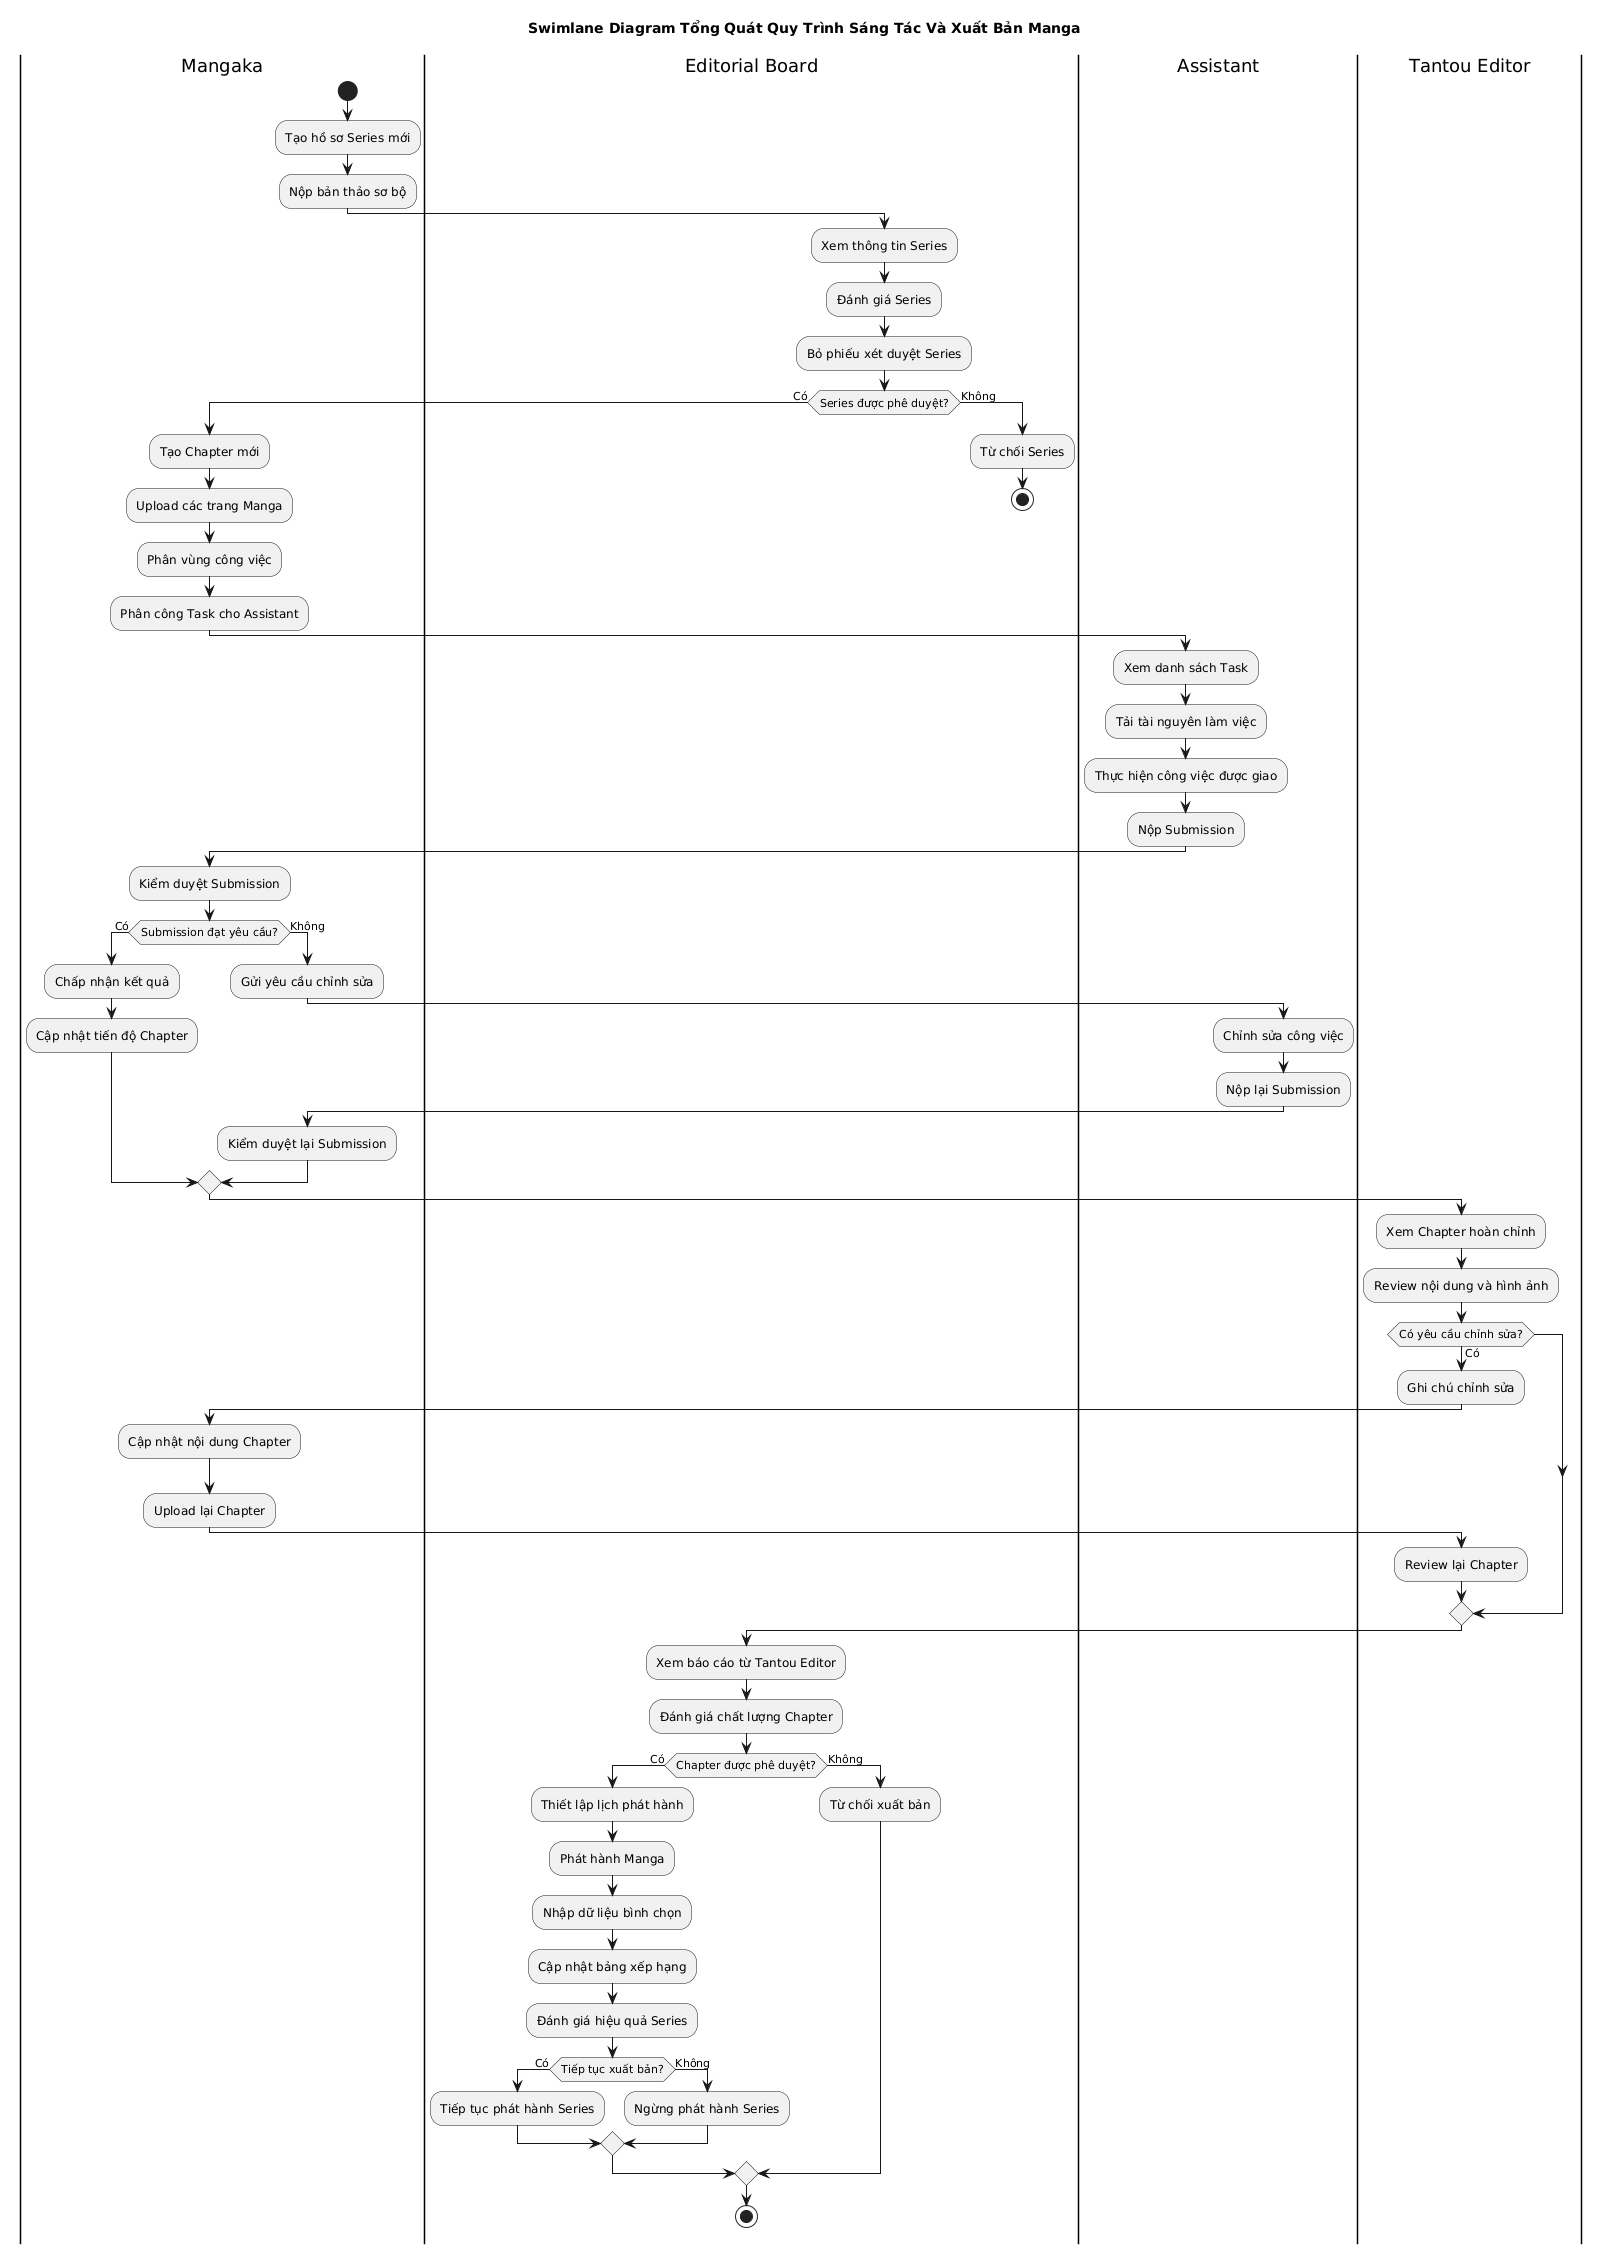
\includegraphics[height=0.75\textheight, width=\textwidth, keepaspectratio]{Chapter3_IMAGE/Swimlane_tong_quat_quy_trinh_sang_tac_maga.png}
    \caption{Swimlane Diagram tổng quát quy trình sáng tác và xuất bản Manga}
    \label{fig:swimlane_manga}
\end{figure}

\FloatBarrier

\subsubsection{Activity Diagram — Giao và thực hiện Task}
\label{subsubsec:act_task}
Activity Diagram này mô tả quy trình phân công và thực hiện công việc giữa Mangaka và Assistant.\\
\indent Quy trình bắt đầu khi Mangaka tạo Task và giao cho Assistant. Sau khi nhận nhiệm vụ, Assistant thực hiện công việc, gửi Submission lên hệ thống và chờ kết quả kiểm duyệt. Trong trường hợp Submission chưa đạt yêu cầu, Assistant sẽ tiếp tục chỉnh sửa và gửi lại cho đến khi được chấp thuận.
\begin{figure}[H]
    \centering
    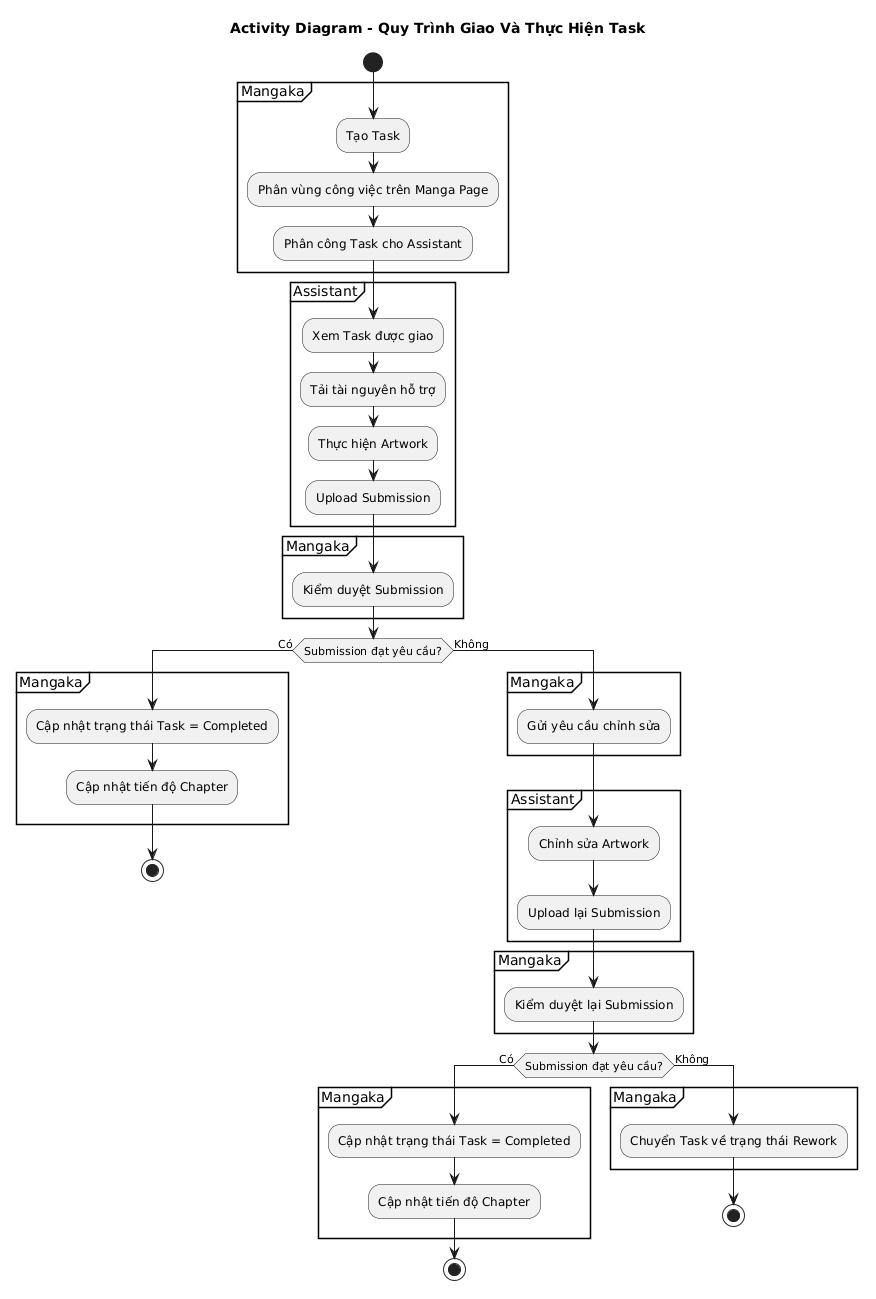
\includegraphics[height=0.75\textheight, width=0.8\textwidth, keepaspectratio]{Chapter3_IMAGE/Activity_Diagram_quy_trinh_giao_va_thuc_hien_Task.png}
    \caption{Activity Diagram quy trình giao và thực hiện Task}
    \label{fig:activity_task}
\end{figure}

\FloatBarrier

\subsubsection{Activity Diagram — Review Chapter}
\label{subsubsec:act_review}
Activity Diagram này mô tả quy trình kiểm duyệt nội dung Manga giữa Mangaka và Tantou Editor.\\
\indent Sau khi Chapter được hoàn thiện, Tantou Editor tiến hành xem xét nội dung và đưa ra phản hồi. Nếu Chapter chưa đạt yêu cầu, Mangaka sẽ thực hiện chỉnh sửa theo nhận xét. Quy trình được lặp lại cho đến khi Chapter được phê duyệt.
\begin{figure}[H]
    \centering
    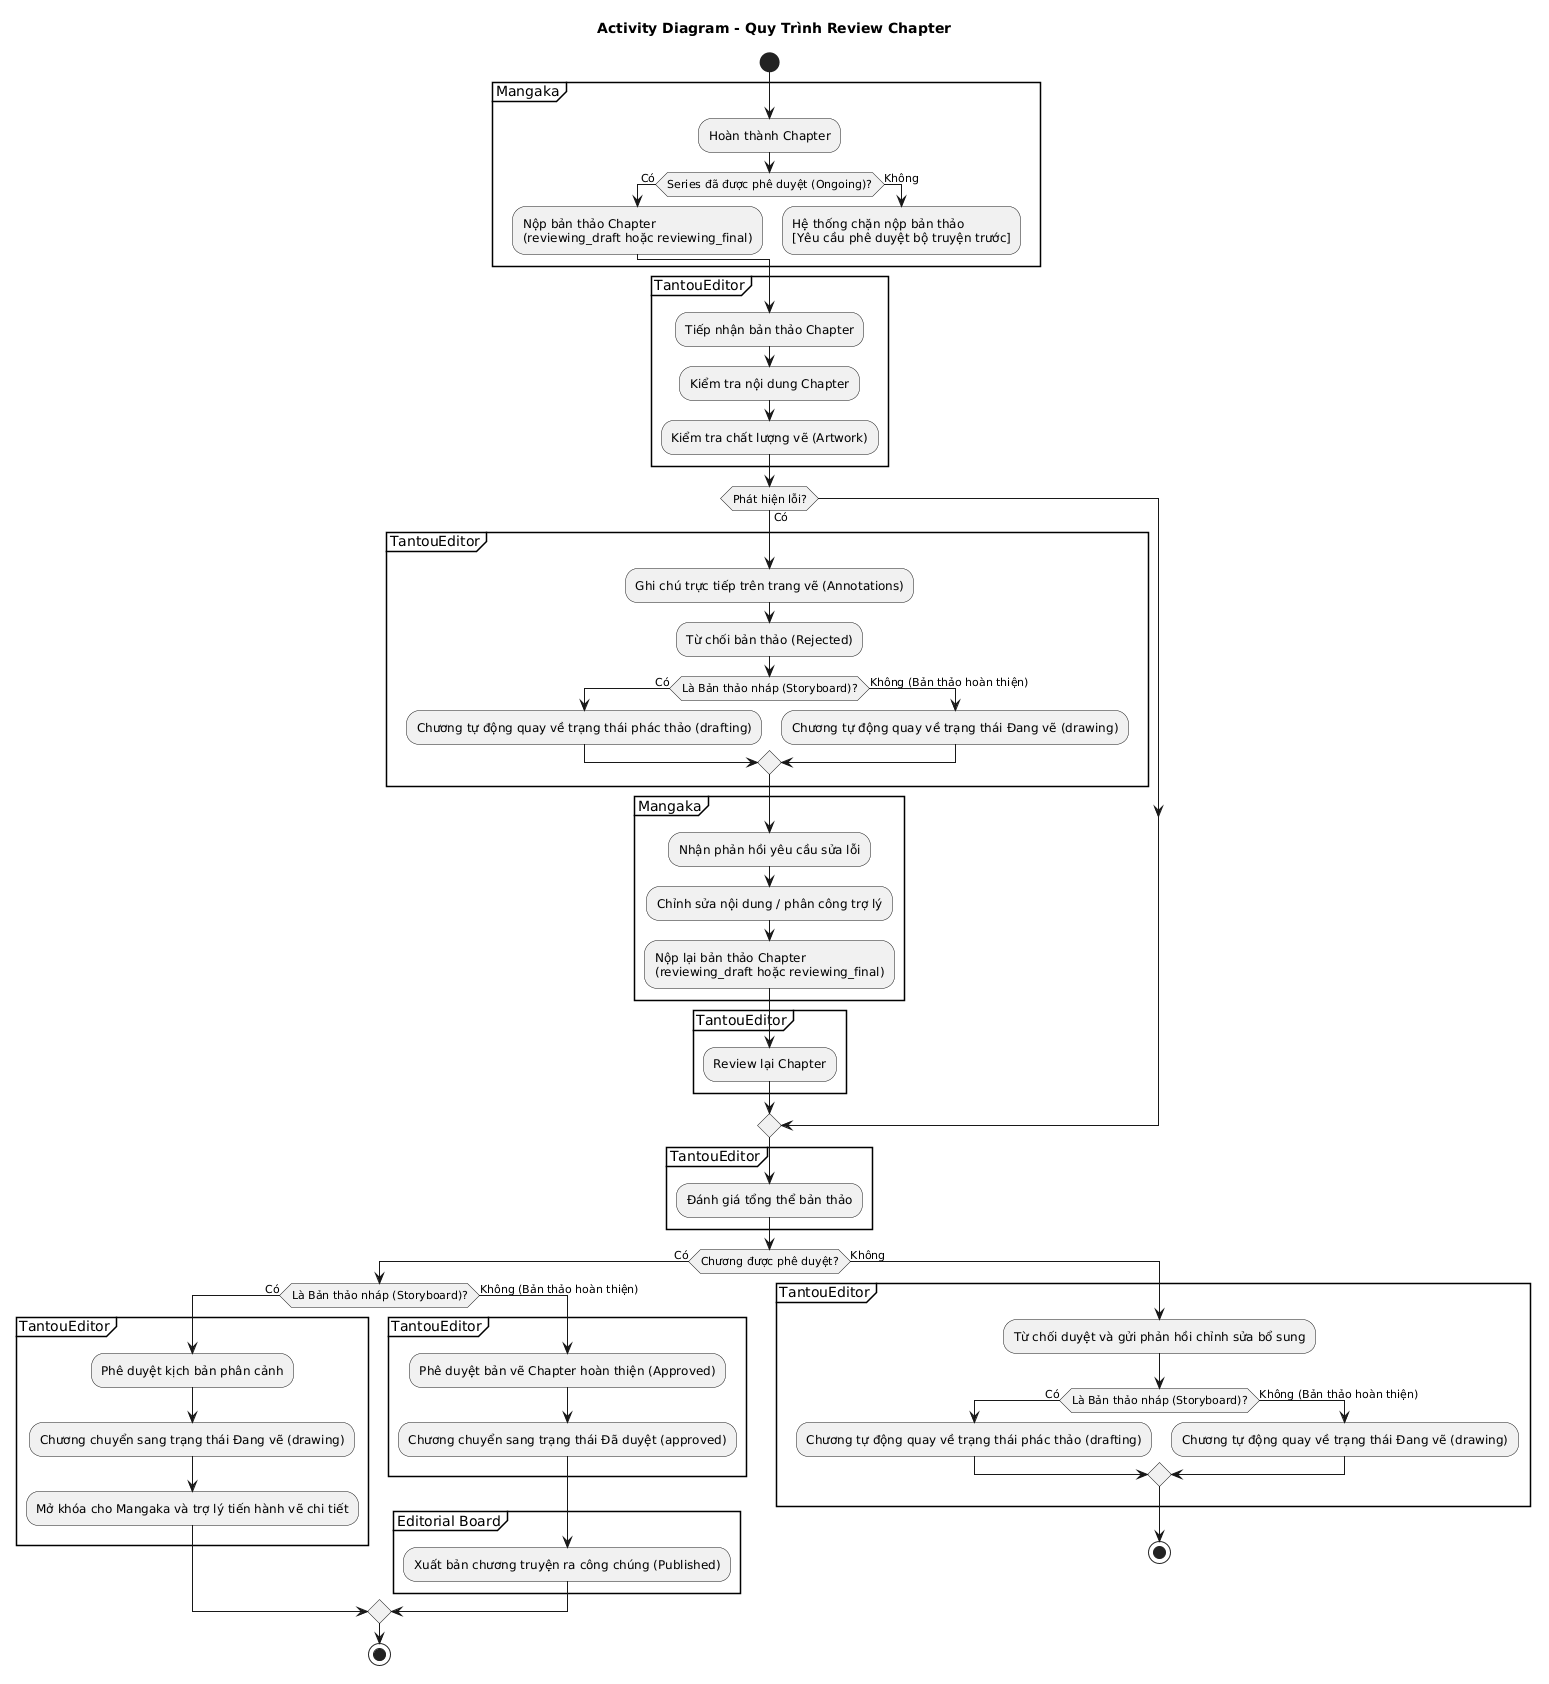
\includegraphics[height=0.75\textheight, width=0.8\textwidth, keepaspectratio]{Chapter3_IMAGE/Activity_Diagram_quy_trinh_Review_Chapter.png}
    \caption{Activity Diagram quy trình Review Chapter}
    \label{fig:activity_review}
\end{figure}

\FloatBarrier

\subsubsection{Activity Diagram — Xuất bản Manga}
\label{subsubsec:act_publish}
Activity Diagram này mô tả quá trình đánh giá và ra quyết định xuất bản đối với một Series Manga.\\
\indent Editorial Board thực hiện cập nhật dữ liệu bình chọn, theo dõi thứ hạng Series và đánh giá hiệu quả phát hành. Dựa trên kết quả đánh giá, hội đồng đưa ra quyết định tiếp tục xuất bản, điều chỉnh kế hoạch phát hành hoặc ngừng phát hành Series.
\begin{figure}[H]
    \centering
    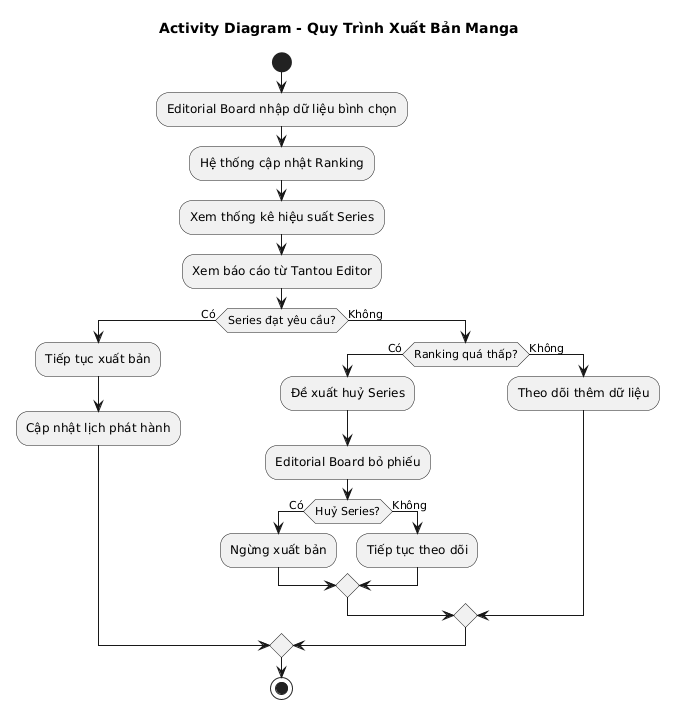
\includegraphics[height=0.75\textheight, width=0.8\textwidth, keepaspectratio]{Chapter3_IMAGE/Activity_Diagram_quy_trinh_xuat_ban_Manga.png}
    \caption{Activity Diagram quy trình xuất bản Manga}
    \label{fig:activity_xuat_ban}
\end{figure}

\FloatBarrier

\subsection{Thiết kế Sequence Diagram}
\label{subsec:sdd_sequence_diagrams}

\subsubsection{Sequence — Đăng nhập hệ thống}
\label{subsubsec:seq_login}
Sequence Diagram mô tả quá trình người dùng đăng nhập vào hệ thống. Hệ thống xác thực thông tin tài khoản và cấp quyền truy cập nếu hợp lệ.

\begin{figure}[H]
    \centering
    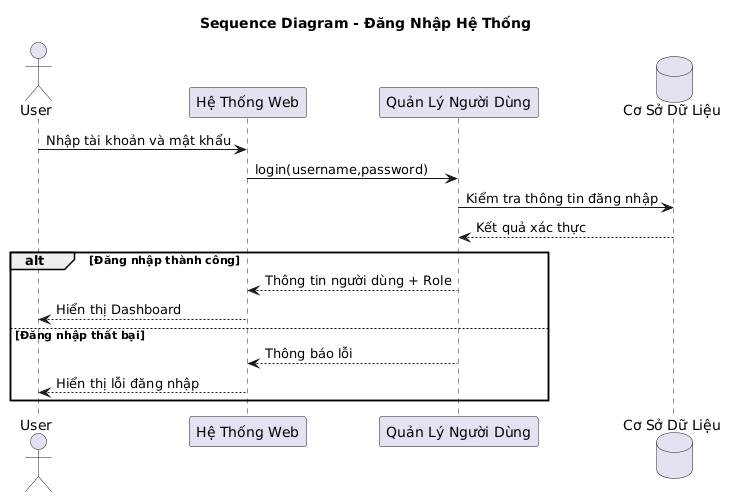
\includegraphics[width=\textwidth]{Chapter3_IMAGE/sequence_diagram_dang_nhap_he_thong.png}
    \caption{Sequence Diagram Đăng nhập hệ thống}
    \label{fig:seq_dang_nhap}
\end{figure}

\subsubsection{Sequence — Phân công Task}
\label{subsubsec:seq_task}
Sequence Diagram mô tả quá trình Manager tạo và phân công công việc cho Assistant. Sau khi Task được tạo, hệ thống lưu thông tin và gửi thông báo đến Assistant.

\begin{figure}[H]
    \centering
    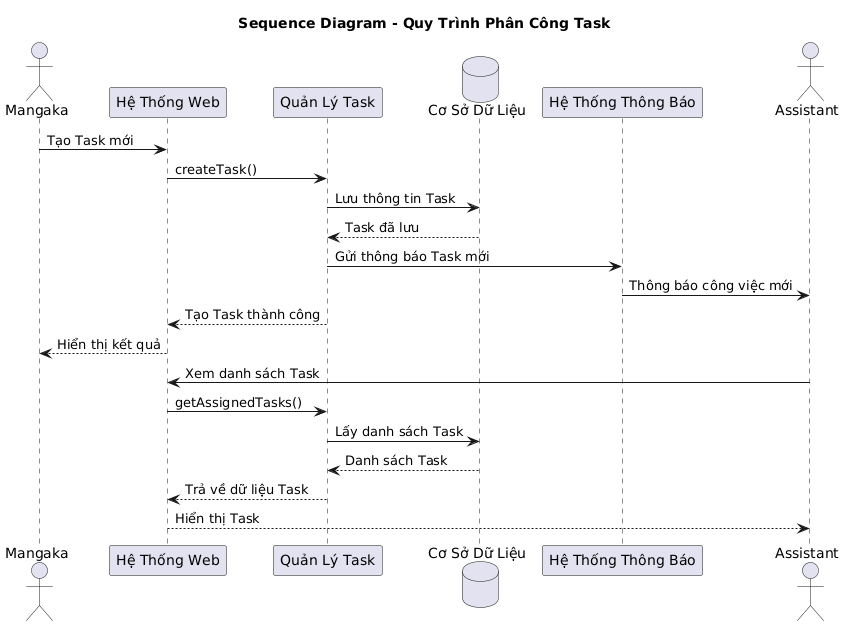
\includegraphics[width=\textwidth]{Chapter3_IMAGE/sequence_diagram_manga_task_assignment.png}
    \caption{Sequence Diagram Phân công Task}
    \label{fig:seq_giao_task}
\end{figure}

\subsubsection{Sequence — Nộp Submission}
\label{subsubsec:seq_submission}
Sequence Diagram mô tả quá trình Assistant nộp kết quả thực hiện Task. Hệ thống lưu Submission và cập nhật trạng thái công việc.

\begin{figure}[H]
    \centering
    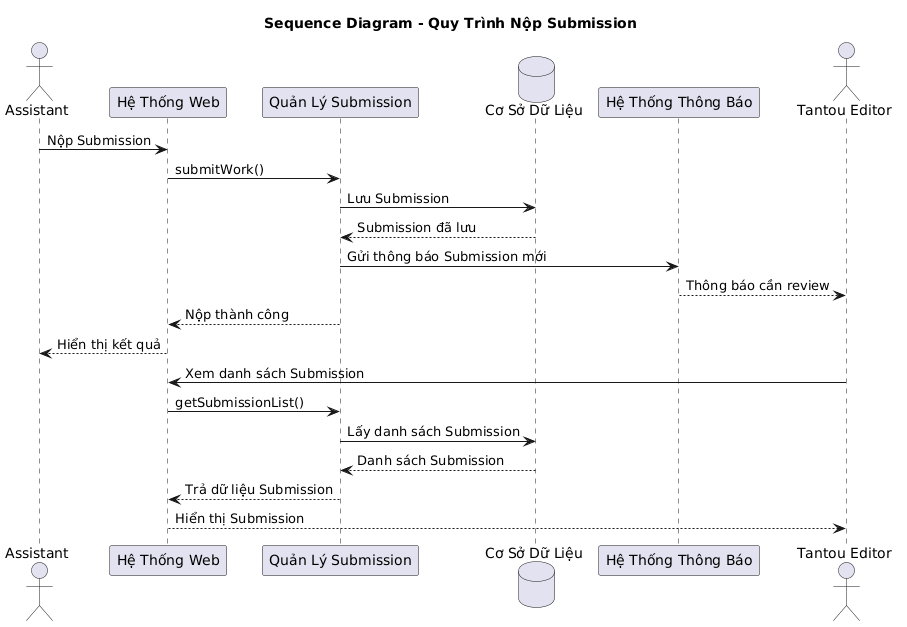
\includegraphics[width=\textwidth]{Chapter3_IMAGE/sequence_diagram_quy_trinh_nop_submission.png}
    \caption{Sequence Diagram Nộp Submission}
    \label{fig:seq_nop_submission}
\end{figure}

\subsubsection{Sequence — Review Chapter}
\label{subsubsec:seq_review}
Sequence Diagram mô tả quá trình Manager đánh giá Submission. Nếu đạt yêu cầu, hệ thống cập nhật tiến độ Chapter; ngược lại hệ thống gửi yêu cầu chỉnh sửa.

\begin{figure}[H]
    \centering
    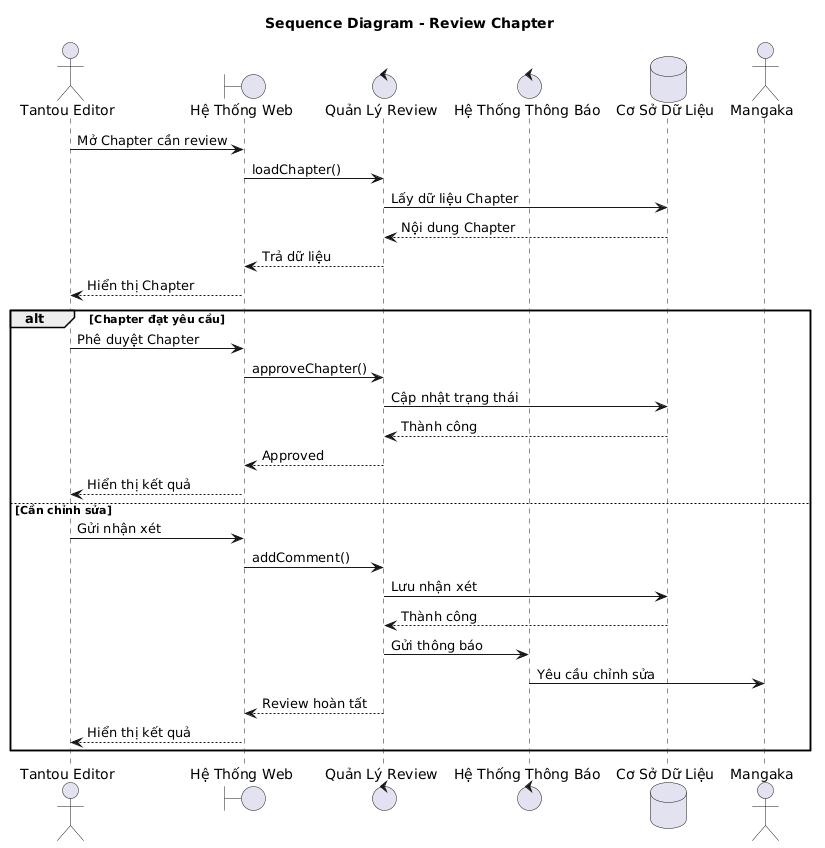
\includegraphics[width=\textwidth]{Chapter3_IMAGE/sequence_diagram_review_chapter.png}
    \caption{Sequence Diagram Review Chapter}
    \label{fig:seq_review_chapter}
\end{figure}

\subsubsection{Sequence — Phê duyệt Xuất bản Series}
\label{subsubsec:seq_publish}
Sequence Diagram mô tả quá trình Hội đồng Biên tập (Editorial Board) tiến hành bỏ phiếu và phê duyệt bộ truyện mới (Series). Hệ thống tự động theo dõi tỷ lệ tán thành và chỉ chuyển trạng thái bộ truyện sang Đang triển khai (Ongoing) khi 100% thành viên Hội đồng đã bỏ phiếu và tỷ lệ tán thành đạt từ 50% trở lên. Sau khi phê duyệt, hệ thống sẽ ghi nhận nhật ký, cập nhật lịch xuất bản, phân công Tantou Editor và gửi thông báo kết quả cho Mangaka.

\begin{figure}[H]
    \centering
    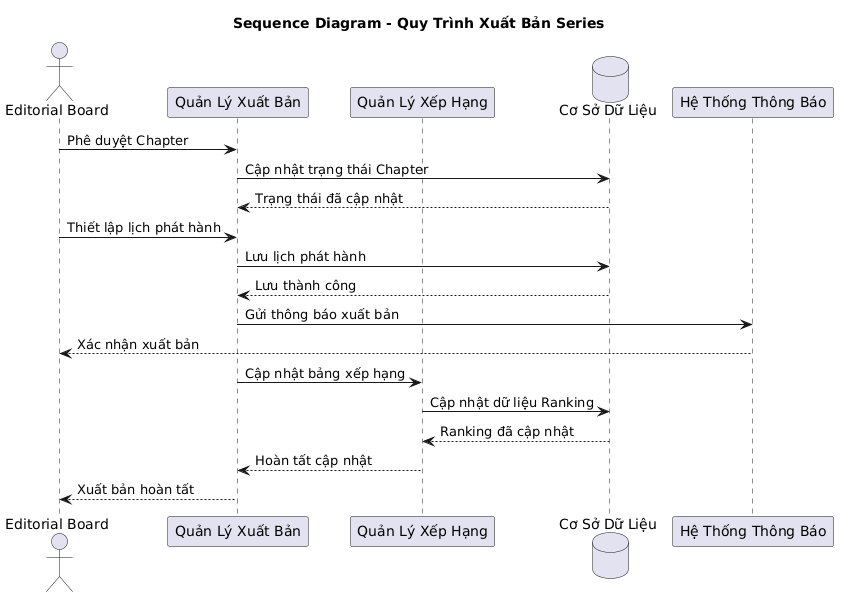
\includegraphics[width=\textwidth]{Chapter3_IMAGE/sequence_diagram_manga_series_publishing.png}
    \caption{Sequence Diagram Phê duyệt Xuất bản Series}
    \label{fig:seq_xuat_ban}
\end{figure}

\subsection{Thiết kế các lớp học}
\label{subsec:sdd_class_diagram}

Class Diagram mô tả cấu trúc tĩnh của hệ thống, bao gồm các lớp chính, thuộc tính, phương thức và mối quan hệ giữa các lớp trong hệ thống quản lý quy trình sản xuất Manga.

\subsubsection{Chi tiết các lớp trong hệ thống}
\label{subsubsec:class_details}

\subsubsection{Lớp Role}
\textit{Mô tả:} Quản lý thông tin vai trò của người dùng trong hệ thống.

\begin{table}[H]
\centering
\renewcommand{\arraystretch}{1.3}
\begin{tabularx}{\textwidth}{|p{4cm}|p{3cm}|>{\raggedright\arraybackslash}X|}
\hline
\rowcolor{tableheader}
\textbf{Thuộc tính} & \textbf{Kiểu dữ liệu} & \textbf{Ý nghĩa} \\ \hline
role\_id & int & Mã vai trò \\ \hline
role\_name & string & Tên vai trò \\ \hline
description & string & Mô tả vai trò \\ \hline
\end{tabularx}
\caption{Đặc tả chi tiết thuộc tính lớp Role}
\label{tab:class_role}
\end{table}


\subsubsection{Lớp User}
\textit{Mô tả:} Quản lý thông tin tài khoản người dùng.

\begin{table}[H]
\centering
\renewcommand{\arraystretch}{1.3}
\begin{tabularx}{\textwidth}{|p{4cm}|p{3cm}|>{\raggedright\arraybackslash}X|}
\hline
\rowcolor{tableheader}
\textbf{Thuộc tính} & \textbf{Kiểu dữ liệu} & \textbf{Ý nghĩa} \\ \hline
user\_id & int & Mã người dùng (Primary Key) \\ \hline
username & string & Tên đăng nhập \\ \hline
full\_name & string & Họ và tên \\ \hline
email & string & Địa chỉ email \\ \hline
password\_hash & string & Mật khẩu đã mã hóa \\ \hline
status & string & Trạng thái tài khoản \\ \hline
is\_head\_board & int & Đánh dấu thành viên là trưởng ban hội đồng xét duyệt \\ \hline
role\_id & int & Mã vai trò (Foreign Key liên kết lớp Role) \\ \hline
\end{tabularx}
\caption{Đặc tả chi tiết thuộc tính lớp User}
\label{tab:class_user}
\end{table}


\subsubsection{Lớp Series}
\textit{Mô tả:} Quản lý thông tin bộ truyện Manga.

\begin{table}[H]
\centering
\renewcommand{\arraystretch}{1.3}
\begin{tabularx}{\textwidth}{|p{4cm}|p{3cm}|>{\raggedright\arraybackslash}X|}
\hline
\rowcolor{tableheader}
\textbf{Thuộc tính} & \textbf{Kiểu dữ liệu} & \textbf{Ý nghĩa} \\ \hline
series\_id & int & Mã bộ truyện (Primary Key) \\ \hline
title & string & Tên bộ truyện \\ \hline
description & string & Mô tả nội dung \\ \hline
status & string & Trạng thái bộ truyện (\texttt{'planning'}, \texttt{'ongoing'}...) \\ \hline
publish\_type & string & Tần suất phát hành (weekly, monthly...) \\ \hline
cover\_image & string & Ảnh bìa bộ truyện \\ \hline
proposal\_file & string & Đường dẫn tệp đề xuất bộ truyện \\ \hline
editor\_id & int & Mã Biên tập viên phụ trách (Foreign Key, cho phép NULL) \\ \hline
dossier\_notes & string & Ghi chú hồ sơ duyệt bộ truyện \\ \hline
mangaka\_id & int & Mã tác giả sở hữu (Foreign Key liên kết lớp User) \\ \hline
\end{tabularx}
\caption{Đặc tả chi tiết thuộc tính lớp Series}
\label{tab:class_series}
\end{table}


\subsubsection{Lớp Chapter}
\textit{Mô tả:} Quản lý thông tin chương truyện.

\begin{table}[H]
\centering
\renewcommand{\arraystretch}{1.3}
\begin{tabularx}{\textwidth}{|p{4cm}|p{3cm}|>{\raggedright\arraybackslash}X|}
\hline
\rowcolor{tableheader}
\textbf{Thuộc tính} & \textbf{Kiểu dữ liệu} & \textbf{Ý nghĩa} \\ \hline
chapter\_id & int & Mã chương (Primary Key) \\ \hline
chapter\_number & int & Số thứ tự chương \\ \hline
title & string & Tên chương \\ \hline
status & string & Trạng thái chương \\ \hline
due\_date & datetime & Hạn hoàn thành chương truyện \\ \hline
published\_at & datetime & Ngày xuất bản \\ \hline
is\_final & tinyint & Đánh dấu chương cuối cùng của bộ truyện \\ \hline
series\_id & int & Mã bộ truyện (Foreign Key liên kết lớp Series) \\ \hline
\end{tabularx}
\caption{Đặc tả chi tiết thuộc tính lớp Chapter}
\label{tab:class_chapter}
\end{table}


\subsubsection{Lớp Page}
\textit{Mô tả:} Quản lý các trang truyện thuộc Chapter.

\begin{table}[H]
\centering
\renewcommand{\arraystretch}{1.3}
\begin{tabularx}{\textwidth}{|p{4cm}|p{3cm}|>{\raggedright\arraybackslash}X|}
\hline
\rowcolor{tableheader}
\textbf{Thuộc tính} & \textbf{Kiểu dữ liệu} & \textbf{Ý nghĩa} \\ \hline
page\_id & int & Mã trang (Primary Key) \\ \hline
page\_number & int & Số thứ tự trang \\ \hline
image\_url & string & Đường dẫn ảnh \\ \hline
old\_image\_url & string & Đường dẫn ảnh cũ trước khi sửa đổi \\ \hline
status & string & Trạng thái hoàn thành \\ \hline
chapter\_id & int & Mã chương (Foreign Key liên kết lớp Chapter) \\ \hline
\end{tabularx}
\caption{Đặc tả chi tiết thuộc tính lớp Page}
\label{tab:class_page}
\end{table}


\subsubsection{Lớp PageRegion}
\textit{Mô tả:} Lưu thông tin phân vùng cụ thể của trang vẽ để phân công công việc.

\begin{table}[H]
\centering
\renewcommand{\arraystretch}{1.3}
\begin{tabularx}{\textwidth}{|p{4cm}|p{3cm}|>{\raggedright\arraybackslash}X|}
\hline
\rowcolor{tableheader}
\textbf{Thuộc tính} & \textbf{Kiểu dữ liệu} & \textbf{Ý nghĩa} \\ \hline
region\_id & int & Mã phân vùng (Primary Key) \\ \hline
region\_type & string & Loại phân vùng (panel, bubble, background...) \\ \hline
x & int & Tọa độ x trên trang truyện \\ \hline
y & int & Tọa độ y trên trang truyện \\ \hline
width & int & Chiều rộng phân vùng \\ \hline
height & int & Chiều cao phân vùng \\ \hline
status & string & Trạng thái hoàn thành phân vùng \\ \hline
page\_id & int & Mã trang truyện chứa phân vùng (Foreign Key liên kết lớp Page) \\ \hline
\end{tabularx}
\caption{Đặc tả chi tiết thuộc tính lớp PageRegion}
\label{tab:class_pageregion}
\end{table}


\subsubsection{Lớp Task}
\textit{Mô tả:} Quản lý công việc được giao cho Assistant.

\begin{table}[H]
\centering
\renewcommand{\arraystretch}{1.3}
\begin{tabularx}{\textwidth}{|p{4cm}|p{3cm}|>{\raggedright\arraybackslash}X|}
\hline
\rowcolor{tableheader}
\textbf{Thuộc tính} & \textbf{Kiểu dữ liệu} & \textbf{Ý nghĩa} \\ \hline
task\_id & int & Mã công việc (Primary Key) \\ \hline
title & string & Tên công việc \\ \hline
task\_type & string & Loại công việc (background, inking, coloring...) \\ \hline
description & string & Mô tả công việc \\ \hline
resource\_url & string & Đường dẫn tệp tài nguyên đính kèm \\ \hline
priority & string & Mức độ ưu tiên \\ \hline
status & string & Trạng thái công việc \\ \hline
due\_date & datetime & Hạn hoàn thành \\ \hline
page\_id & int & Mã trang truyện liên kết (Foreign Key liên kết lớp Page) \\ \hline
page\_region\_id & int & Mã phân vùng liên quan (Foreign Key, cho phép NULL) \\ \hline
grouped\_region\_ids & string & Danh sách các phân vùng gộp liên quan (cho phép NULL) \\ \hline
mangaka\_id & int & Mã tác giả giao việc (Foreign Key liên kết lớp User) \\ \hline
assistant\_id & int & Mã trợ lý nhận việc (Foreign Key liên kết lớp User) \\ \hline
\end{tabularx}
\caption{Đặc tả chi tiết thuộc tính lớp Task}
\label{tab:class_task}
\end{table}


\subsubsection{Lớp Submission}
\textit{Mô tả:} Quản lý các sản phẩm được nộp lên hệ thống.

\begin{table}[H]
\centering
\renewcommand{\arraystretch}{1.3}
\begin{tabularx}{\textwidth}{|p{4cm}|p{3cm}|>{\raggedright\arraybackslash}X|}
\hline
\rowcolor{tableheader}
\textbf{Thuộc tính} & \textbf{Kiểu dữ liệu} & \textbf{Ý nghĩa} \\ \hline
submission\_id & int & Mã bài nộp (Primary Key) \\ \hline
file\_url & string & Đường dẫn tập tin \\ \hline
notes & string & Ghi chú bổ sung \\ \hline
status & string & Trạng thái bài nộp \\ \hline
submitted\_at & datetime & Thời gian nộp \\ \hline
task\_id & int & Mã công việc liên kết (Foreign Key liên kết lớp Task, cho phép NULL) \\ \hline
chapter\_id & int & Mã chương liên kết (Foreign Key liên kết lớp Chapter, cho phép NULL) \\ \hline
user\_id & int & Mã người nộp (Foreign Key liên kết lớp User) \\ \hline
\end{tabularx}
\caption{Đặc tả chi tiết thuộc tính lớp Submission}
\label{tab:class_submission}
\end{table}


\subsubsection{Lớp Review}
\textit{Mô tả:} Quản lý các đánh giá và phản hồi đối với Submission.

\begin{table}[H]
\centering
\renewcommand{\arraystretch}{1.3}
\begin{tabularx}{\textwidth}{|p{4cm}|p{3cm}|>{\raggedright\arraybackslash}X|}
\hline
\rowcolor{tableheader}
\textbf{Thuộc tính} & \textbf{Kiểu dữ liệu} & \textbf{Ý nghĩa} \\ \hline
review\_id & int & Mã đánh giá (Primary Key) \\ \hline
comments & string & Nội dung nhận xét \\ \hline
rating & int & Điểm đánh giá \\ \hline
created\_at & datetime & Thời gian đánh giá \\ \hline
submission\_id & int & Mã bài nộp được đánh giá (Foreign Key liên kết lớp Submission) \\ \hline
reviewer\_id & int & Mã người đánh giá (Foreign Key liên kết lớp User) \\ \hline
\end{tabularx}
\caption{Đặc tả chi tiết thuộc tính lớp Review}
\label{tab:class_review}
\end{table}


\subsubsection{Lớp EditorAnnotation}
\textit{Mô tả:} Lưu thông tin ghi chú lỗi trực quan vẽ đè trên trang truyện từ Editor.

\begin{table}[H]
\centering
\renewcommand{\arraystretch}{1.3}
\begin{tabularx}{\textwidth}{|p{4cm}|p{3cm}|>{\raggedright\arraybackslash}X|}
\hline
\rowcolor{tableheader}
\textbf{Thuộc tính} & \textbf{Kiểu dữ liệu} & \textbf{Ý nghĩa} \\ \hline
annotation\_id & int & Mã ghi chú (Primary Key) \\ \hline
x & int & Tọa độ x của vùng đánh dấu nét lỗi \\ \hline
y & int & Tọa độ y của vùng đánh dấu nét lỗi \\ \hline
width & int & Chiều rộng vùng lỗi \\ \hline
height & int & Chiều cao vùng lỗi \\ \hline
comments & string & Nhận xét, góp ý chi tiết \\ \hline
created\_at & datetime & Thời gian tạo ghi chú \\ \hline
page\_id & int & Mã trang truyện liên quan (Foreign Key liên kết lớp Page) \\ \hline
editor\_id & int & Mã Biên tập viên ghi chú (Foreign Key liên kết lớp User) \\ \hline
\end{tabularx}
\caption{Đặc tả chi tiết thuộc tính lớp EditorAnnotation}
\label{tab:class_editorannotation}
\end{table}


\subsubsection{Lớp SubmissionAnnotation}
\textit{Mô tả:} Lưu trữ thông tin ghi chú báo lỗi trực quan vẽ đè của Tác giả (Mangaka) trên các bản vẽ nộp của Trợ lý.

\begin{table}[H]
\centering
\renewcommand{\arraystretch}{1.3}
\begin{tabularx}{\textwidth}{|p{4cm}|p{3cm}|>{\raggedright\arraybackslash}X|}
\hline
\rowcolor{tableheader}
\textbf{Thuộc tính} & \textbf{Kiểu dữ liệu} & \textbf{Ý nghĩa} \\ \hline
annotation\_id & int & Mã ghi chú lỗi (Primary Key) \\ \hline
x & int & Tọa độ x của vùng báo lỗi trên hình ảnh nộp \\ \hline
y & int & Tọa độ y của vùng báo lỗi trên hình ảnh nộp \\ \hline
width & int & Chiều rộng vùng báo lỗi \\ \hline
height & int & Chiều cao vùng báo lỗi \\ \hline
comments & string & Ghi chú mô tả lỗi chi tiết \\ \hline
created\_at & datetime & Thời gian tạo ghi chú \\ \hline
submission\_id & int & Mã bản nộp của Trợ lý liên quan (Foreign Key liên kết lớp Submission) \\ \hline
user\_id & int & Mã Tác giả thực hiện ghi chú (Foreign Key liên kết lớp User) \\ \hline
\end{tabularx}
\caption{Đặc tả chi tiết thuộc tính lớp SubmissionAnnotation}
\label{tab:class_submissionannotation}
\end{table}


\subsubsection{Lớp BoardVote}
\textit{Mô tả:} Lưu trữ phiếu biểu quyết của thành viên Hội đồng biên tập cho đề xuất Series.

\begin{table}[H]
\centering
\renewcommand{\arraystretch}{1.3}
\begin{tabularx}{\textwidth}{|p{4cm}|p{3cm}|>{\raggedright\arraybackslash}X|}
\hline
\rowcolor{tableheader}
\textbf{Thuộc tính} & \textbf{Kiểu dữ liệu} & \textbf{Ý nghĩa} \\ \hline
vote\_id & int & Mã phiếu bầu (Primary Key) \\ \hline
vote & string & Quyết định bầu chọn (approve/reject) \\ \hline
created\_at & datetime & Thời gian bỏ phiếu \\ \hline
series\_id & int & Mã bộ truyện liên quan (Foreign Key liên kết lớp Series) \\ \hline
board\_member\_id & int & Mã thành viên hội đồng bỏ phiếu (Foreign Key liên kết lớp User) \\ \hline
\end{tabularx}
\caption{Đặc tả chi tiết thuộc tính lớp BoardVote}
\label{tab:class_boardvote}
\end{table}


\subsubsection{Lớp SeriesRanking}
\textit{Mô tả:} Quản lý thông tin xếp hạng của các bộ truyện.

\begin{table}[H]
\centering
\renewcommand{\arraystretch}{1.3}
\begin{tabularx}{\textwidth}{|p{4cm}|p{3cm}|>{\raggedright\arraybackslash}X|}
\hline
\rowcolor{tableheader}
\textbf{Thuộc tính} & \textbf{Kiểu dữ liệu} & \textbf{Ý nghĩa} \\ \hline
ranking\_id & int & Mã xếp hạng (Primary Key) \\ \hline
rank\_position & int & Thứ hạng \\ \hline
score & decimal & Điểm đánh giá \\ \hline
votes & int & Số lượng phiếu bầu trong kỳ \\ \hline
period\_start\_date & date & Thời điểm bắt đầu kỳ xếp hạng \\ \hline
series\_id & int & Mã bộ truyện được xếp hạng (Foreign Key liên kết lớp Series) \\ \hline
board\_member\_id & int & Mã thành viên BBT chấm điểm (Foreign Key liên kết lớp User) \\ \hline
\end{tabularx}
\caption{Đặc tả chi tiết thuộc tính lớp SeriesRanking}
\label{tab:class_seriesranking}
\end{table}


\subsubsection{Lớp Notification}
\textit{Mô tả:} Quản lý thông báo gửi đến người dùng.

\begin{table}[H]
\centering
\renewcommand{\arraystretch}{1.3}
\begin{tabularx}{\textwidth}{|p{4cm}|p{3cm}|>{\raggedright\arraybackslash}X|}
\hline
\rowcolor{tableheader}
\textbf{Thuộc tính} & \textbf{Kiểu dữ liệu} & \textbf{Ý nghĩa} \\ \hline
notification\_id & int & Mã thông báo (Primary Key) \\ \hline
type & string & Loại thông báo \\ \hline
message & string & Nội dung thông báo \\ \hline
is\_read & boolean & Trạng thái đã đọc \\ \hline
related\_id & int & ID của thực thể liên quan (task, submission...) \\ \hline
user\_id & int & Mã người dùng nhận (Foreign Key liên kết lớp User) \\ \hline
\end{tabularx}
\caption{Đặc tả chi tiết thuộc tính lớp Notification}
\label{tab:class_notification}
\end{table}


\subsubsection{Lớp SystemLog}
\textit{Mô tả:} Lưu thông tin nhật ký các hoạt động nhạy cảm trong hệ thống.

\begin{table}[H]
\centering
\renewcommand{\arraystretch}{1.3}
\begin{tabularx}{\textwidth}{|p{4cm}|p{3cm}|>{\raggedright\arraybackslash}X|}
\hline
\rowcolor{tableheader}
\textbf{Thuộc tính} & \textbf{Kiểu dữ liệu} & \textbf{Ý nghĩa} \\ \hline
log\_id & int & Mã log (Primary Key) \\ \hline
action & string & Tên hành động thực hiện \\ \hline
details & string & Mô tả chi tiết \\ \hline
ip\_address & string & Địa chỉ IP truy cập \\ \hline
created\_at & datetime & Thời gian ghi nhận log \\ \hline
user\_id & int & Mã người dùng thực hiện (Foreign Key liên kết lớp User, có thể NULL) \\ \hline
\end{tabularx}
\caption{Đặc tả chi tiết thuộc tính lớp SystemLog}
\label{tab:class_systemlog}
\end{table}


\subsubsection{Bổ sung phương thức (Methods)}
\label{subsubsec:class_methods}

Các phương thức (Methods) của từng lớp trong hệ thống mô tả chi tiết chữ ký hàm (Method Signatures) bao gồm tham số truyền vào, kiểu dữ liệu trả về và ý nghĩa hoạt động thực tế trong mã nguồn PHP Model:

\begin{itemize}
    \item \textbf{Lớp Role:}
    \begin{itemize}
        \item \texttt{findByRoleName(roleName: string): Role}\\
            Lấy thông tin vai trò theo tên (ví dụ: 'mangaka', 'assistant'...).
        \item \texttt{getRolesWithUserCount(): array}\\
            Lấy danh sách vai trò kèm theo số lượng người dùng thuộc vai trò đó.
    \end{itemize}
    
    \item \textbf{Lớp User:}
    \begin{itemize}
        \item \texttt{findByEmail(email: string): array}\\
            Tìm người dùng theo email đăng ký.
        \item \texttt{findByUsername(username: string): array}\\
            Tìm người dùng theo tên đăng nhập.
        \item \texttt{getUserByIdWithRole(id: int): array}\\
            Lấy thông tin người dùng kèm theo tên vai trò tương ứng.
        \item \texttt{findByRoleName(roleName: string): array}\\
            Lấy danh sách người dùng đang active theo tên vai trò.
        \item \texttt{getRoleStatistics(): array}\\
            Lấy dữ liệu thống kê số lượng tài khoản theo từng vai trò.
        \item \texttt{getAllUsersWithRole(): array}\\
            Lấy danh sách tất cả người dùng trong hệ thống cùng vai trò của họ.
        \item \texttt{getPaginatedUsers(limit: int, offset: int): array}\\
            Lấy danh sách người dùng phân trang phục vụ trang quản trị Admin.
        \item \texttt{demoteOtherHeads(exceptUserId: int): bool}\\
            Bãi nhiệm vai trò Trưởng ban hội đồng của các thành viên khác khi có Trưởng ban mới được bổ nhiệm.
    \end{itemize}

    \item \textbf{Lớp Series:}
    \begin{itemize}
        \item \texttt{findByMangakaId(mangakaId: int): array}\\
            Lấy danh sách các bộ truyện của tác giả đang đăng nhập.
        \item \texttt{findByStatus(status: string): array}\\
            Lấy danh sách các bộ truyện theo trạng thái (ongoing, planning...).
        \item \texttt{getSeriesByEditorId(editorId: int): array}\\
            Lấy danh sách các bộ truyện được phân công cho Biên tập viên và đã duyệt phát hành.
        \item \texttt{getSeriesForPublishing(): array}\\
            Lấy danh sách bộ truyện kèm thống kê số chương, điểm số phục vụ cho Hội đồng duyệt xuất bản.
        \item \texttt{getDossiersByEditorId(editorId: int): array}\\
            Lấy danh sách hồ sơ truyện theo Biên tập viên phụ trách.
        \item \texttt{countActiveSeries(): int}\\
            Đếm số lượng bộ truyện đang hoạt động trong hệ thống.
        \item \texttt{isTitleExists(title: string, excludeId: int = null): bool}\\
            Kiểm tra xem tên truyện đã tồn tại trên hệ thống chưa để tránh trùng tên.
    \end{itemize}

    \item \textbf{Lớp Chapter:}
    \begin{itemize}
        \item \texttt{findBySeriesId(seriesId: int): array}\\
            Lấy danh sách các chương thuộc bộ truyện, sắp xếp tăng dần.
        \item \texttt{isChapterNumberExists(seriesId: int, chapterNumber: int): bool}\\
            Kiểm tra số chương đã tồn tại trong bộ truyện chưa để tránh trùng lặp.
        \item \texttt{findByMangakaId(mangakaId: int): array}\\
            Lấy danh sách chương truyện của Mangaka sở hữu.
        \item \texttt{findBySeriesIdWithStats(seriesId: int): array}\\
            Lấy danh sách chương truyện kèm thống kê số lượng Task hoàn thành của trợ lý.
        \item \texttt{hasFinalChapter(seriesId: int): bool}\\
            Kiểm tra xem truyện đã có chương cuối cùng (is\_final = 1) chưa.
        \item \texttt{countUnfinishedChapters(seriesId: int): int}\\
            Đếm số chương chưa hoàn tất của một truyện.
        \item \texttt{hasFinalApprovedChapter(seriesId: int): bool}\\
            Kiểm tra xem chương cuối đã được duyệt hay chưa.
        \item \texttt{getUpcomingDeadlinesByEditor(editorId: int): array}\\
            Lấy danh sách các chương sắp đến hạn nộp thuộc BTV quản lý.
        \item \texttt{findPublishedChapters(): array}\\
            Lấy danh sách các chương đã xuất bản (published) thuộc các Series.
        \item \texttt{findByMangakaIdWithStats(mangakaId: int): array}\\
            Lấy danh sách chương truyện kèm thống kê số lượng Task hoàn thành và nộp bài cho Mangaka.
        \item \texttt{countByMangakaId(mangakaId: int): int}\\
            Đếm tổng số chương truyện do Mangaka quản lý/sở hữu.
        \item \texttt{findApprovedChapters(): array}\\
            Lấy tất cả các chương truyện đã ở trạng thái được phê duyệt hoàn thiện (approved).
    \end{itemize}

    \item \textbf{Lớp Page:}
    \begin{itemize}
        \item \texttt{findByChapterId(chapterId: int): array}\\
            Lấy danh sách các trang vẽ thuộc chương, sắp xếp theo số trang.
        \item \texttt{isPageNumberExists(chapterId: int, pageNumber: int): bool}\\
            Kiểm tra trùng số trang trong một chương.
        \item \texttt{findByChapterIdWithAnnotationCount(chapterId: int): array}\\
            Lấy danh sách trang vẽ kèm số lỗi ghi chú của Biên tập viên.
        \item \texttt{getPageNumbersByChapterId(chapterId: int): array}\\
            Lấy mảng các số thứ tự trang hiện có trong chương.
        \item \texttt{getOtherPageNumbers(chapterId: int, pageId: int): array}\\
            Lấy số thứ tự các trang khác trong chương để phục vụ thay đổi vị trí.
        \item \texttt{updateStatusByChapterId(chapterId: int, status: string): bool}\\
            Cập nhật trạng thái cho tất cả các trang thuộc một chương truyện cụ thể.
        \item \texttt{findByMangakaId(mangakaId: int): array}\\
            Lấy danh sách các trang vẽ do trợ lý nộp thuộc quyền quản lý của Mangaka.
        \item \texttt{countByMangakaId(mangakaId: int): int}\\
            Đếm số lượng trang vẽ do Mangaka tạo ra trên hệ thống.
    \end{itemize}

    \item \textbf{Lớp PageRegion:}
    \begin{itemize}
        \item \texttt{findByPageId(pageId: int): array}\\
            Lấy tất cả các phân vùng của một trang truyện cụ thể.
        \item \texttt{findByIds(ids: array): array}\\
            Tìm các phân vùng trên trang dựa theo danh sách ID truyền vào.
    \end{itemize}

    \item \textbf{Lớp Task:}
    \begin{itemize}
        \item \texttt{findByPageId(pageId: int): array}\\
            Lấy danh sách các công việc trên một trang truyện cụ thể kèm tên trợ lý.
        \item \texttt{findByAssistantId(assistantId: int): array}\\
            Lấy danh sách công việc được giao của trợ lý kèm thông tin chương, trang, phân vùng.
        \item \texttt{findActiveByAssistantId(assistantId: int): array}\\
            Lấy các công việc chưa hoàn thành của một trợ lý.
        \item \texttt{findByMangakaId(mangakaId: int): array}\\
            Lấy danh sách công việc do tác giả giao cho các trợ lý.
        \item \texttt{getStatusStatistics(): array}\\
            Lấy thống kê số lượng Task theo trạng thái (pending, in\_progress, completed).
        \item \texttt{getMonthlyIncomeStats(assistantId: int): array}\\
            Tính toán thống kê thu nhập dự kiến của trợ lý theo từng tháng dựa trên số Task hoàn thành.
        \item \texttt{findTasksByChapterId(chapterId: int): array}\\
            Tìm danh sách toàn bộ Task liên kết với các trang trong một Chapter.
        \item \texttt{findByPageRegionIds(regionIds: array): array}\\
            Tìm các Task liên quan đến danh sách ID phân vùng.
        \item \texttt{deleteActiveTasksByRegionIds(regionIds: array): bool}\\
            Xóa nhanh các Task đang hoạt động liên kết với danh sách phân vùng.
        \item \texttt{countByPageAndAssistant(pageId: int, assistantId: int): int}\\
            Đếm số Task được giao cho trợ lý cụ thể trên một trang truyện.
        \item \texttt{countByAssistantIdWithGating(assistantId: int): int}\\
            Đếm số Task trợ lý đang thực hiện để thực hiện giới hạn nhận việc tối đa (Gating).
    \end{itemize}

    \item \textbf{Lớp Submission:}
    \begin{itemize}
        \item \texttt{findByTaskId(taskId: int): array}\\
            Lấy lịch sử các lần nộp bài vẽ cho một Task cụ thể.
        \item \texttt{findByChapterId(chapterId: int): array}\\
            Lấy danh sách các lần nộp bản thảo cho một chương cụ thể.
        \item \texttt{findPendingSubmissions(): array}\\
            Lấy danh sách các bản thảo chương đang chờ duyệt của hệ thống.
        \item \texttt{countPendingChapterSubmissionsByEditor(editorId: int): int}\\
            Đếm số lượng chương đang chờ duyệt thuộc Biên tập viên quản lý.
        \item \texttt{getStatusStatistics(): array}\\
            Lấy thống kê số lượng bài nộp theo trạng thái.
        \item \texttt{countByMangakaId(mangakaId: int): int}\\
            Đếm tổng số bài nộp do Trợ lý thực hiện dưới quyền của Mangaka.
        \item \texttt{countPendingByMangakaId(mangakaId: int): int}\\
            Đếm số bài nộp đang chờ duyệt thuộc quyền quản lý của Mangaka.
        \item \texttt{findByUserId(userId: int): array}\\
            Lấy danh sách các bản nộp dựa theo ID người nộp (User ID).
        \item \texttt{findPendingSubmissionsByEditorId(editorId: int): array}\\
            Lấy các bản nộp chương/task đang chờ Biên tập viên chuyên trách phê duyệt.
        \item \texttt{findAllChapterSubmissionsByEditorId(editorId: int): array}\\
            Lấy toàn bộ lịch sử bản nộp chương liên kết với Biên tập viên.
        \item \texttt{findAllTaskSubmissionsByMangakaId(mangakaId: int): array}\\
            Lấy toàn bộ lịch sử nộp bài vẽ phân vùng của Trợ lý cho Mangaka.
        \item \texttt{findWithMetadataById(id: int): array}\\
            Lấy chi tiết bản nộp kèm thông tin siêu dữ liệu (metadata) của Chapter và Task liên quan.
        \item \texttt{findAllChapterSubmissions(): array}\\
            Lấy toàn bộ danh sách nộp bản thảo Chapter trong hệ thống.
    \end{itemize}

    \item \textbf{Lớp Review:}
    \begin{itemize}
        \item \texttt{findBySubmissionId(submissionId: int): array}\\
            Lấy danh sách nhận xét cho một lần nộp bài cụ thể.
        \item \texttt{countReviewsByEditor(editorId: int, status: string): int}\\
            Đếm số lượng đánh giá của Editor theo trạng thái bài nộp.
        \item \texttt{findByReviewerId(reviewerId: int): array}\\
            Lấy danh sách các phản hồi, đánh giá được thực hiện bởi người dùng.
    \end{itemize}

    \item \textbf{Lớp EditorAnnotation:}
    \begin{itemize}
        \item \texttt{findByPageId(pageId: int): array}\\
            Lấy danh sách các ghi chú báo lỗi của Editor trên trang truyện kèm theo tên Editor.
        \item \texttt{deleteByPageId(pageId: int): bool}\\
            Xóa toàn bộ các ghi chú báo lỗi trên một trang truyện cụ thể.
    \end{itemize}

    \item \textbf{Lớp SubmissionAnnotation:}
    \begin{itemize}
        \item \texttt{findBySubmissionId(submissionId: int): array}\\
            Lấy danh sách ghi chú lỗi trực quan trên bản nộp của trợ lý kèm tên đầy đủ người đánh giá.
    \end{itemize}

    \item \textbf{Lớp BoardVote:}
    \begin{itemize}
        \item \texttt{castVote(seriesId: int, memberId: int, vote: string): bool}\\
            Ghi nhận lượt bỏ phiếu của thành viên hội đồng cho đề xuất truyện.
        \item \texttt{getMemberVote(seriesId: int, memberId: int): string}\\
            Lấy ý kiến bỏ phiếu hiện tại của một thành viên cụ thể.
        \item \texttt{getApprovalStats(seriesId: int): array}\\
            Tính toán động tỉ lệ phần trăm tán thành và số lượng phiếu bầu đạt được.
    \end{itemize}

    \item \textbf{Lớp SeriesRanking:}
    \begin{itemize}
        \item \texttt{findBySeriesId(seriesId: int): array}\\
            Lấy danh sách lịch sử điểm số và thứ hạng của bộ truyện.
        \item \texttt{getSeriesCountByPeriod(period: string): int}\\
            Đếm số lượng bộ truyện đã xếp hạng trong một kỳ đánh giá cụ thể.
        \item \texttt{getTopSeriesByPeriod(period: string, limit: int): array}\\
            Lấy danh sách các bộ truyện có điểm cao nhất trong kỳ đánh giá.
        \item \texttt{getBottomSeriesByPeriod(period: string, limit: int): array}\\
            Lấy danh sách các bộ truyện có điểm thấp nhất trong kỳ đánh giá.
        \item \texttt{getLatestPeriod(): string}\\
            Lấy kỳ xếp hạng gần nhất hiện có trên hệ thống.
        \item \texttt{getPreviousRanking(seriesId: int, period: string): array}\\
            Lấy thông tin thứ hạng và điểm số của bộ truyện trong kỳ đánh giá trước đó.
        \item \texttt{checkDuplicateRanking(seriesId: int, period: string): bool}\\
            Kiểm tra xem bộ truyện đã có bản ghi xếp hạng trong kỳ tương ứng chưa.
        \item \texttt{findByMangakaId(mangakaId: int): array}\\
            Lấy lịch sử xếp hạng của các bộ truyện thuộc Mangaka sở hữu.
        \item \texttt{getLatestRanking(): array}\\
            Lấy danh sách xếp hạng mới nhất của các bộ truyện.
        \item \texttt{findWithDetails(id: int): array}\\
            Lấy chi tiết bản xếp hạng kèm thông tin bộ truyện và ban biên tập liên quan.
        \item \texttt{findAllWithSeries(): array}\\
            Lấy toàn bộ lịch sử xếp hạng tất cả các bộ truyện trên hệ thống.
    \end{itemize}

    \item \textbf{Lớp Notification:}
    \begin{itemize}
        \item \texttt{createNotification(userId: int, type: string, message: string, relatedId: int = null): bool}\\
            Tạo và gửi thông báo mới cho người dùng.
        \item \texttt{findByUserId(userId: int): array}\\
            Lấy toàn bộ danh sách thông báo của người dùng.
        \item \texttt{findUnreadByUserId(userId: int): array}\\
            Lấy danh sách các thông báo chưa đọc của người dùng.
        \item \texttt{getUnreadCount(userId: int): int}\\
            Đếm số lượng thông báo chưa đọc của người dùng.
        \item \texttt{getLatestNotifications(userId: int, limit: int = 5): array}\\
            Lấy danh sách thông báo mới nhất phục vụ hiển thị nhanh (dropdown).
        \item \texttt{markAsRead(notificationId: int, userId: int): bool}\\
            Đánh dấu một thông báo cụ thể là đã đọc.
        \item \texttt{markAllAsRead(userId: int): bool}\\
            Đánh dấu toàn bộ thông báo của người dùng là đã đọc.
        \item \texttt{findAllWithUser(): array}\\
            Lấy danh sách toàn bộ thông báo của mọi người dùng kèm tên chi tiết.
        \item \texttt{getTypeDetails(type: string): array}\\
            Lấy thông tin chi tiết (badge màu, tên hiển thị) theo từng loại thông báo.
    \end{itemize}

    \item \textbf{Lớp SystemLog:}
    \begin{itemize}
        \item \texttt{logAction(userId: int, action: string, details: string): bool}\\
            Ghi nhận nhật ký hoạt động nghiệp vụ của người dùng vào hệ thống.
        \item \texttt{getPaginatedLogs(limit: int, offset: int): array}\\
            Lấy danh sách log có phân trang kèm theo thông tin chi tiết người dùng thực hiện.
    \end{itemize}
\end{itemize}

\subsection{Thiết kế biểu đồ trạng thái (State Machine Diagram)}
\label{subsec:sdd_state_machine}

Biểu đồ trạng thái (State Machine Diagram) được sử dụng để mô tả chi tiết vòng đời hoạt động và các sự kiện chuyển trạng thái của các thực thể cốt lõi trong hệ thống:

\subsubsection{Biểu đồ trạng thái Chương truyện (Chapter)}
\label{subsubsec:state_chapter}
Mô tả vòng đời của chương truyện từ khi là bản thảo thô cho đến khi xuất bản chính thức.
\begin{figure}[H]
    \centering
    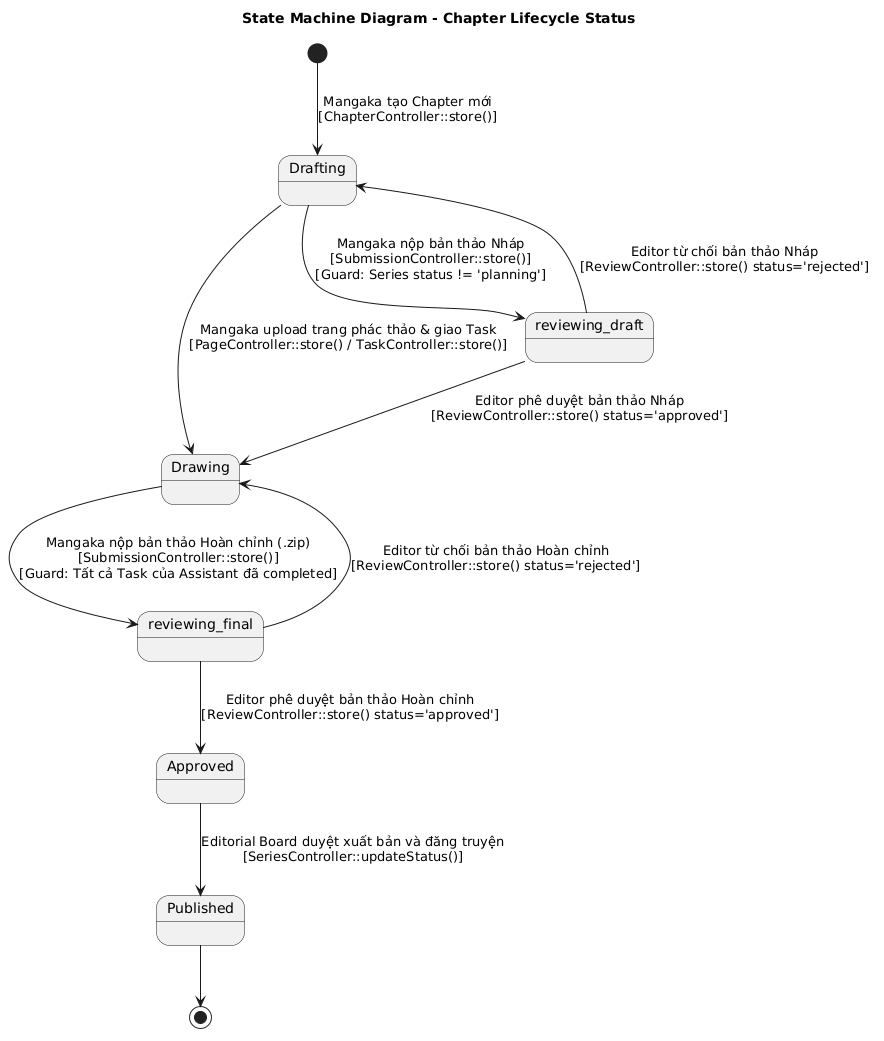
\includegraphics[width=0.9\textwidth]{Chapter3_IMAGE/State_Machine_Chapter.png}
    \caption{Biểu đồ trạng thái của Chương truyện (Chapter)}
    \label{fig:state_chapter}
\end{figure}

\subsubsection{Biểu đồ trạng thái Trang truyện (Page)}
\label{subsubsec:state_page}
Mô tả sự dịch chuyển trạng thái vẽ của một trang Manga cụ thể khi có sự tác động phân công công việc.
\begin{figure}[H]
    \centering
    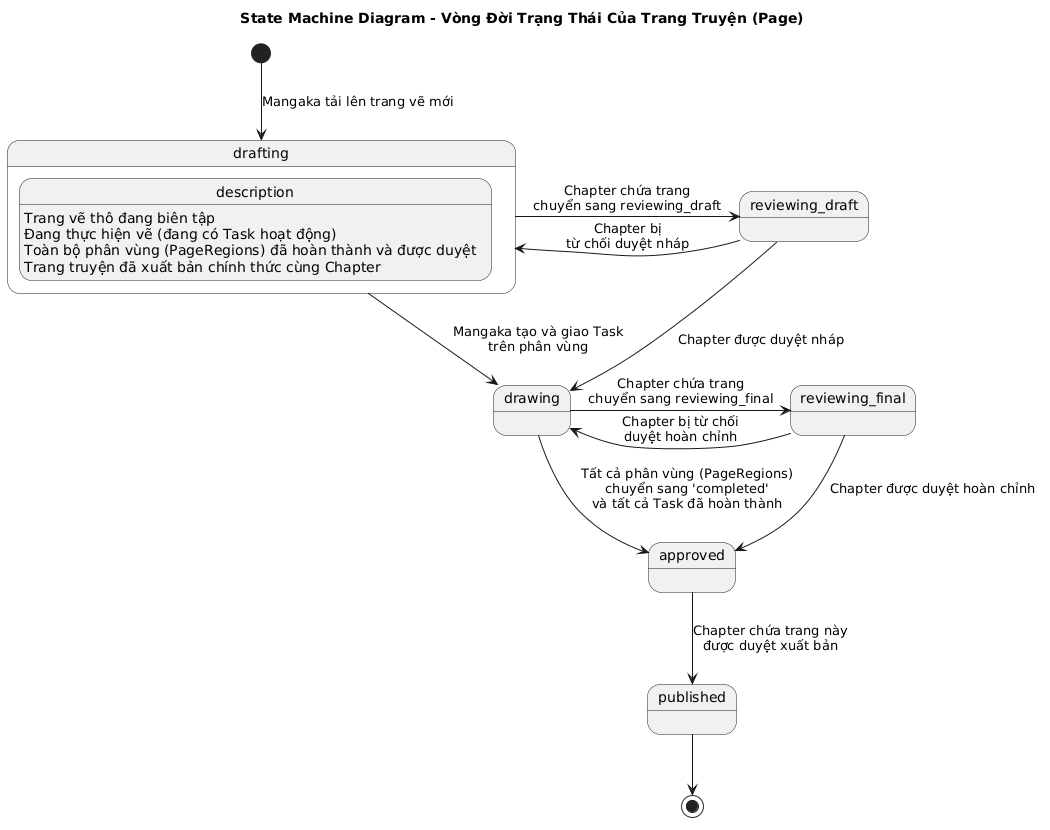
\includegraphics[width=0.8\textwidth]{Chapter3_IMAGE/State_Machine_Page.png}
    \caption{Biểu đồ trạng thái của Trang truyện (Page)}
    \label{fig:state_page}
\end{figure}

\subsubsection{Biểu đồ trạng thái Phân vùng trang truyện (PageRegion)}
\label{subsubsec:state_pageregion}
Mô tả vòng đời của một phân vùng ảnh vẽ tay nhỏ trên trang truyện từ khi được đánh dấu cho đến khi hoàn thành.
\begin{figure}[H]
    \centering
    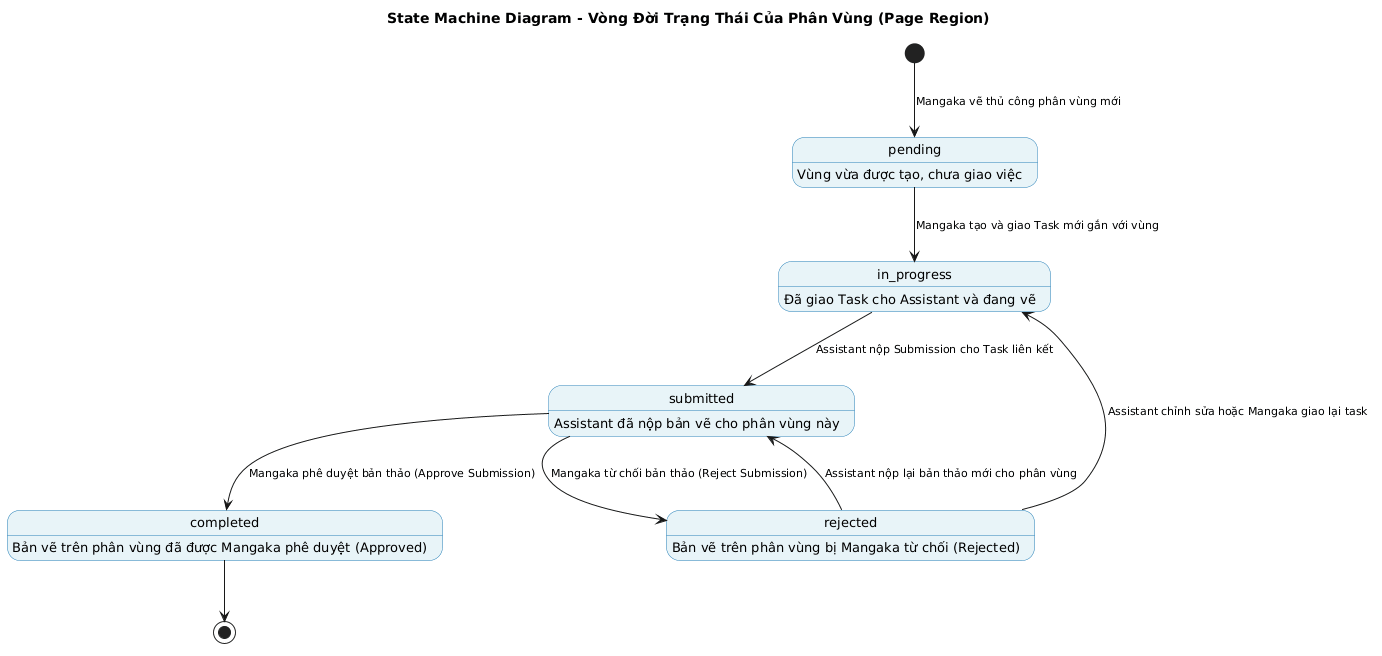
\includegraphics[width=0.8\textwidth]{Chapter3_IMAGE/State_Machine_Page_Region.png}
    \caption{Biểu đồ trạng thái của Phân vùng trang truyện (PageRegion)}
    \label{fig:state_pageregion}
\end{figure}

\subsubsection{Biểu đồ trạng thái Bộ truyện Manga (Series)}
\label{subsubsec:state_series}
Mô tả vòng đời của dự án truyện Manga từ đề xuất kế hoạch, sáng tác thực tế đến khi kết thúc hoặc đình bản.
\begin{figure}[H]
    \centering
    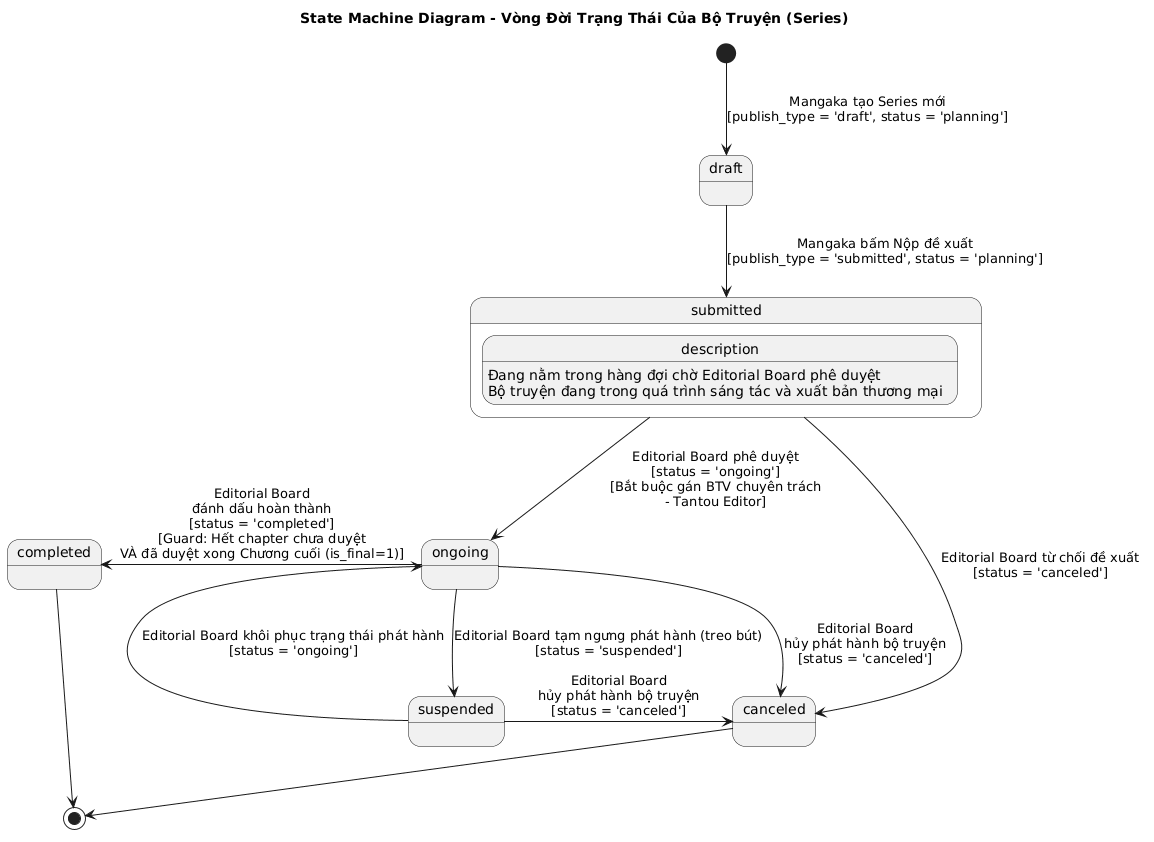
\includegraphics[width=0.8\textwidth]{Chapter3_IMAGE/State_Machine_Series.png}
    \caption{Biểu đồ trạng thái của Bộ truyện (Series)}
    \label{fig:state_series}
\end{figure}

\subsubsection{Biểu đồ trạng thái Công việc giao trợ lý (Task)}
\label{subsubsec:state_task}
Mô tả tiến độ phân công, tiếp nhận và hoàn thiện các Task vẽ hỗ trợ của các Assistant.
\begin{figure}[H]
    \centering
    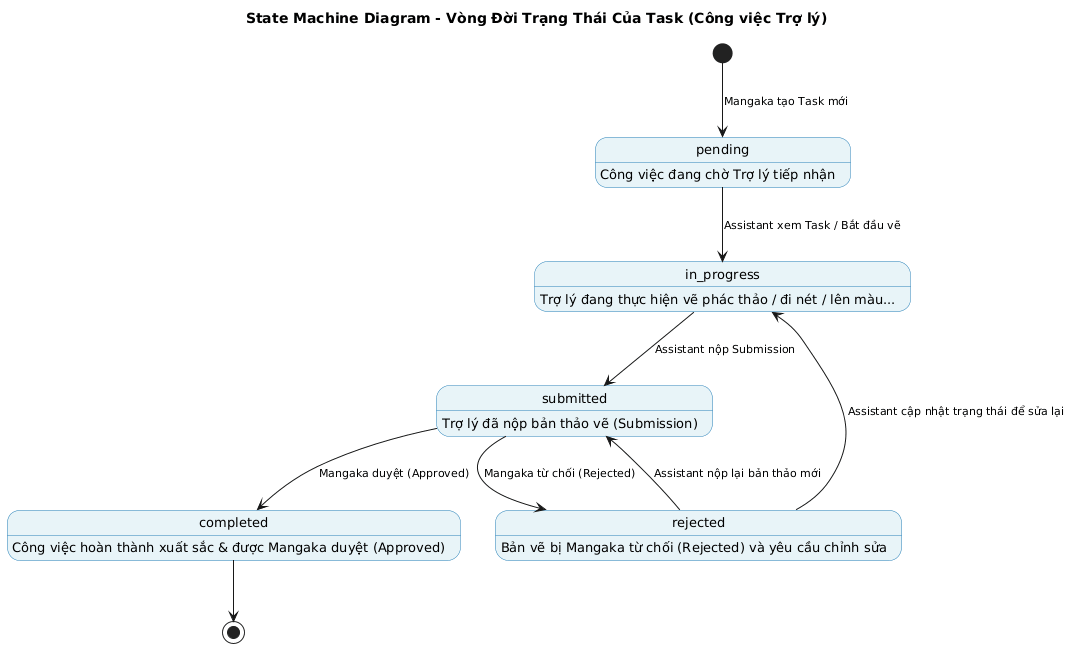
\includegraphics[width=0.8\textwidth]{Chapter3_IMAGE/State_Machine_Task.png}
    \caption{Biểu đồ trạng thái của Công việc (Task)}
    \label{fig:state_task}
\end{figure}

\subsubsection{Class Diagram tổng thể}
\label{subsubsec:class_overview}

Class Diagram tổng thể thể hiện toàn bộ các lớp cốt lõi của hệ thống cùng các mối quan hệ liên kết, kế thừa và phụ thuộc giữa chúng.

\begin{figure}[H]
    \centering
    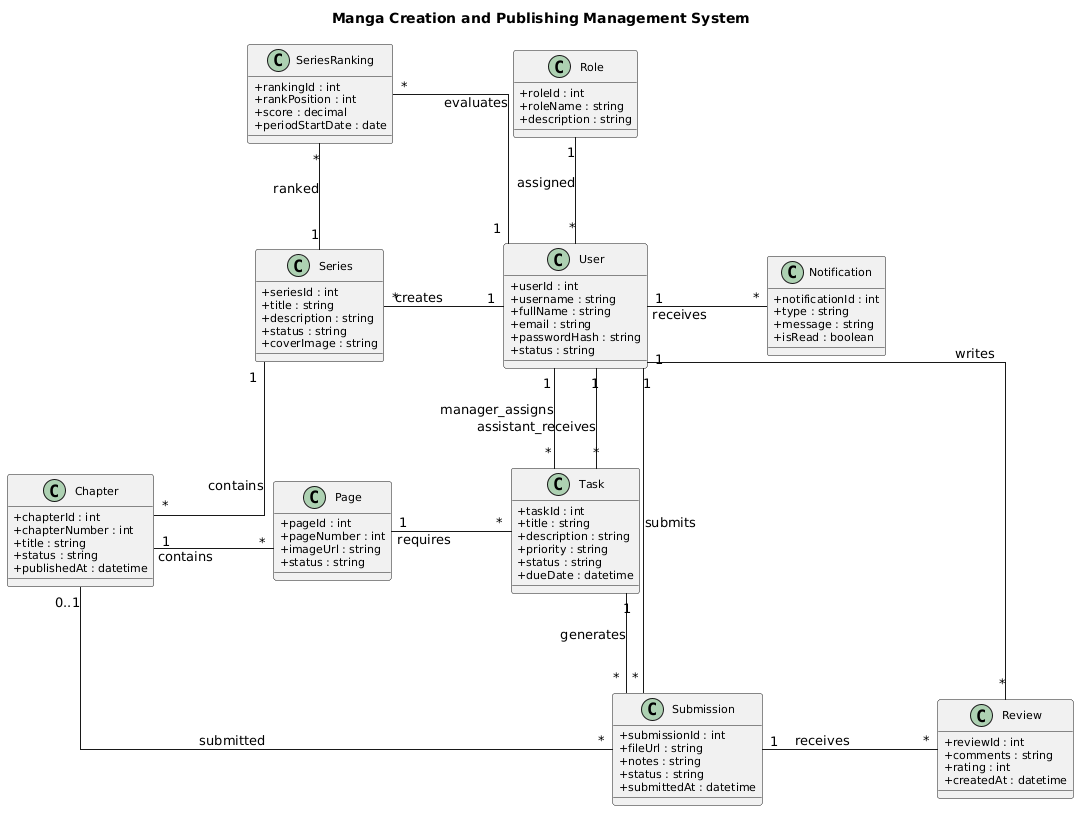
\includegraphics[width=\textwidth, height=0.9\textheight, keepaspectratio]{Chapter3_IMAGE/class_diagram.png}
    \caption{Class Diagram tổng thể}
    \label{fig:class_diagram_tong_the}
\end{figure}

\subsubsection{Mô tả các mối quan hệ}
\label{subsubsec:class_relationships}

Các mối quan hệ (Association/Multiplicity) giữa các lớp trong Class Diagram thể hiện luồng nghiệp vụ và tương tác dữ liệu cốt lõi của hệ thống, bao gồm:

\begin{itemize}
    \item \textbf{Role (1) - (*) User:} Một vai trò (VD: Admin, Manager, Assistant, Editor) có thể được gán cho nhiều người dùng. Mỗi người dùng bắt buộc thuộc về một vai trò nhất định để phân quyền hệ thống.
    \item \textbf{User (1) - (*) Series:} Một tác giả (Mangaka) có thể sáng tác và quản lý nhiều bộ truyện (Series) khác nhau.
    \item \textbf{Series (1) - (*) Chapter:} Một bộ truyện bao gồm nhiều chương (Chapter) nối tiếp nhau.
    \item \textbf{Chapter (1) - (*) Page:} Mỗi chương truyện bao gồm nhiều trang (Page) cụ thể chứa hình ảnh nội dung truyện.
    \item \textbf{User (1) - (*) Task:} Người dùng đóng vai trò giao việc (Manager/Mangaka) có thể phân công nhiều công việc (Task). Đồng thời, người dùng đóng vai trò nhận việc (Assistant) có thể tiếp nhận và thực hiện nhiều Task.
    \item \textbf{Task (1) - (*) Submission:} Một công việc được giao có thể tạo ra nhiều bản nộp (Submission) khác nhau nếu yêu cầu phải nộp lại nhiều lần.
    \item \textbf{Submission (1) - (*) Review:} Mỗi bản nộp của Assistant có thể nhận được nhiều lượt đánh giá, phản hồi (Review) từ cấp trên để chỉnh sửa cho hoàn thiện.
    \item \textbf{Submission (1) - (*) SubmissionAnnotation:} Mỗi bản nộp (Submission) của Trợ lý có thể nhận được nhiều ghi chú lỗi trực quan (SubmissionAnnotation) từ Mangaka để phục vụ chỉnh sửa.
    \item \textbf{User (1) - (*) SubmissionAnnotation:} Tác giả (Mangaka) có thể tạo nhiều ghi chú lỗi trực quan trên các bản nộp khác nhau.
    \item \textbf{Series (1) - (*) SeriesRanking:} Mỗi bộ truyện sẽ được đánh giá và lưu lịch sử qua nhiều kỳ xếp hạng (SeriesRanking) khác nhau dựa trên điểm số (score) và phiếu bình chọn (votes) thu thập được.
    \item \textbf{User (1) - (*) SeriesRanking:} Ban biên tập (User) là những người thực hiện đánh giá và cập nhật xếp hạng cho các bộ truyện.
    \item \textbf{User (1) - (*) Notification:} Mỗi người dùng sẽ có hộp thư chứa nhiều thông báo (Notification) từ hệ thống để cập nhật tiến độ công việc hoặc kết quả duyệt bài.
\end{itemize}


\subsection{Thiết kế giao diện người dùng (UI Design)}
\label{subsec:sdd_ui_design}

\subsubsection{Dashboard}
\label{subsubsec:ui_dashboard}

\subsubsection{Trang đăng nhập}
\label{subsubsec:ui_login}

\subsubsection{Quản lý Series}
\label{subsubsec:ui_series}

\subsubsection{Quản lý Chapter}
\label{subsubsec:ui_chapter}

\subsubsection{Quản lý Task}
\label{subsubsec:ui_task}

\subsubsection{Nộp Submission}
\label{subsubsec:ui_submission}

\subsubsection{Review}
\label{subsubsec:ui_review}

\subsubsection{Thông báo}
\label{subsubsec:ui_notification}

\subsubsection{Xếp hạng}
\label{subsubsec:ui_ranking}


\chapter{Tài liệu kiểm thử phần mềm (Software Testing Documentation)}
\label{ch:kiem_thu}

\section{Phạm vi kiểm thử (Scope of Testing)}
\label{sec:test_scope}

Tài liệu này xác định phạm vi kiểm thử cho hệ thống quản lý quy trình sáng tác và xuất bản Manga (Manga Creation Workflow and Publishing Management System). Phạm vi bao gồm cả kiểm thử chức năng và phi chức năng nhằm đảm bảo hệ thống vận hành đúng đặc tả yêu cầu phần mềm (SRS).

\begin{itemize}
    \item \textbf{Kiểm thử trong phạm vi (In-Scope):}
    \begin{itemize}
        \item Toàn bộ các chức năng cốt lõi của hệ thống từ các ca sử dụng đặc tả (UC-01 đến UC-33): Quản lý người dùng, phân quyền truy cập, quản lý Series, Chapter, Page, giao và thực hiện Task, nộp bản thảo (Submission), đánh giá bản thảo (Review), xét duyệt Series, xuất bản, nhập dữ liệu bình chọn độc giả, cập nhật xếp hạng Series và gửi nhận thông báo.
        \item Các yêu cầu phi chức năng (NFR) đã được định lượng: Hiệu năng tải trang ảnh và phản hồi API, các cơ chế bảo mật xác thực/phân quyền, khả năng tương thích hiển thị (Responsive) trên màn hình thiết bị di động/máy tính bảng, tính sẵn sàng khi ngắt kết nối tạm thời.
    \end{itemize}
    \item \textbf{Kiểm thử ngoài phạm vi (Out-of-Scope):}
    \begin{itemize}
        \item Kiểm thử bảo mật tầng sâu của máy chủ hạ tầng (OS patching, network level DDoS defense).
        \item Kiểm thử các tích hợp thanh toán (Payment gateways) của bên thứ ba không thuộc phạm vi phần mềm quản lý nội bộ.
        \item Kiểm thử hiệu năng mạng và băng thông của nhà cung cấp dịch vụ Internet (ISP).
    \end{itemize}
\end{itemize}

\section{Chiến lược kiểm thử (Test Strategy)}
\label{sec:test_strategy}

Chiến lược kiểm thử áp dụng mô hình kiểm thử nhiều tầng nhằm phát hiện sớm lỗi và đảm bảo chất lượng phần mềm xuyên suốt các giai đoạn phát triển:

\begin{itemize}
    \item \textbf{Các cấp độ kiểm thử (Testing Levels):}
    \begin{itemize}
        \item \textit{Kiểm thử đơn vị (Unit Testing):} Do đội ngũ lập trình viên tự thực hiện trên các module code riêng lẻ. Tỷ lệ phủ mã nguồn tối thiểu phải đạt $80\%$.
        \item \textit{Kiểm thử tích hợp (Integration Testing):} Thực hiện kiểm tra tính đúng đắn khi tích hợp các dịch vụ API, cơ sở dữ liệu và các module nghiệp vụ kết nối với nhau.
        \item \textit{Kiểm thử hệ thống (System Testing):} Tiến hành kiểm thử luồng nghiệp vụ khép kín (End-to-End) trên môi trường Staging tích hợp đầy đủ giao diện người dùng và cơ sở dữ liệu.
        \item \textit{Kiểm thử chấp nhận người dùng (User Acceptance Testing - UAT):} Do đại diện các bên liên quan thực tế (như Mangaka, Assistant và Tantou Editor) thực hiện kiểm thử trên các kịch bản thực tế để nghiệm thu chất lượng phần mềm.
    \end{itemize}
    \item \textbf{Phương pháp kiểm thử (Testing Methodology):}
    \begin{itemize}
        \item \textit{Kiểm thử hộp đen (Black-box Testing):} Áp dụng chủ yếu để kiểm thử chức năng giao diện, dựa vào đặc tả ca sử dụng mà không cần biết cấu trúc mã nguồn bên trong.
        \item \textit{Kiểm thử tự động (Automated Testing):} Sử dụng các công cụ tự động hóa để chạy kiểm thử hồi quy (regression testing) cho các API backend.
        \item \textit{Kiểm thử thủ công (Manual Testing):} Áp dụng cho kiểm thử giao diện người dùng (UI/UX), tính tương thích responsive trên các trình duyệt và thiết bị di động.
    \end{itemize}
    \item \textbf{Phân loại mức độ nghiêm trọng của lỗi (Defect Severity):}
    \begin{itemize}
        \item \textit{Mức 1 (Critical):} Lỗi gây sập hệ thống, mất mát dữ liệu cơ sở dữ liệu, hoặc vi phạm bảo mật nghiêm trọng (rò rỉ bản quyền truyện).
        \item \textit{Mức 2 (Major):} Lỗi chức năng nghiệp vụ cốt lõi không hoạt động và không có giải pháp tạm thời (ví dụ: Mangaka không thể tạo Task mới, Assistant không thể nộp bài vẽ).
        \item \textit{Mức 3 (Minor):} Lỗi giao diện hiển thị, căn lề lệch, sai chính tả văn bản tiếng Việt hoặc cảnh báo không ảnh hưởng nghiêm trọng đến luồng nghiệp vụ.
    \end{itemize}
\end{itemize}

\section{Kế hoạch kiểm thử (Test Plan)}
\label{sec:test_plan}

Kế hoạch kiểm thử chi tiết hóa việc phân bổ tài nguyên, thiết lập môi trường và quy trình nghiệm thu chất lượng:

\begin{itemize}
    \item \textbf{Môi trường kiểm thử (Test Environment):}
    \begin{itemize}
        \item Máy chủ Staging chạy trên nền tảng Docker/Linux đồng bộ cấu hình với máy chủ Production.
        \item Cơ sở dữ liệu Staging được populate sẵn dữ liệu thử nghiệm (ít nhất 5 tài khoản người dùng tương ứng với các vai trò, 10 Series truyện mẫu, và 100 trang vẽ thô).
        \item Thiết bị kiểm thử: Máy tính chạy Google Chrome, Safari, Firefox; Điện thoại di động (iPhone và Android) hỗ trợ kiểm tra responsive.
    \end{itemize}
    \item \textbf{Tiêu chí bắt đầu và kết thúc (Entrance \& Exit Criteria):}
    \begin{itemize}
        \item \textit{Tiêu chí bắt đầu (Entrance Criteria):} Mã nguồn đã hoàn thiện biên dịch không lỗi; Toàn bộ các Unit Test đã được chạy thành công; Môi trường Staging đã sẵn sàng hoạt động ổn định; Kịch bản kiểm thử đã được phê duyệt.
        \item \textit{Tiêu chí kết thúc (Exit Criteria):} 100\% các kịch bản kiểm thử (TC-01 đến TC-15) được thực hiện đầy đủ; Không còn tồn đọng lỗi mức Critical và Major; Tỷ lệ Pass Rate đạt tối thiểu $95\%$.
    \end{itemize}
\end{itemize}

\section{Kịch bản kiểm thử (Test Cases)}
\label{sec:test_cases}

Dưới đây là 15 kịch bản kiểm thử (Test Cases) chi tiết bao gồm thông tin về Actor, tiền điều kiện, các bước thực hiện và kết quả mong đợi nhằm kiểm tra các tính năng và ràng buộc cốt lõi của hệ thống:

\subsection{TC-01: Đăng nhập — thông tin hợp lệ}
\label{subsec:tc01_login_valid}
\begin{itemize}
    \item \textbf{Mục tiêu:} Xác thực người dùng đăng nhập thành công khi nhập đúng thông tin tài khoản.
    \item \textbf{Actor thực hiện:} Bất kỳ người dùng nào (Admin, Mangaka, Assistant, Tantou Editor, Editorial Board).
    \item \textbf{Tiền điều kiện:} Tài khoản đã được tạo và kích hoạt trên hệ thống (ví dụ: username \code{mangaka\_test}, vai trò Mangaka).
    \item \textbf{Các bước thực hiện:}
    \begin{enumerate}
        \item Truy cập trang đăng nhập của hệ thống.
        \item Nhập Tên đăng nhập hợp lệ vào ô Username.
        \item Nhập Mật khẩu hợp lệ vào ô Password.
        \item Nhấn nút "Đăng nhập".
    \end{enumerate}
    \item \textbf{Kết quả mong đợi:} Đăng nhập thành công, hệ thống thiết lập phiên làm việc (session) hợp lệ, chuyển hướng người dùng về trang Dashboard tương ứng với vai trò Mangaka, và hiển thị thông điệp chào mừng.
\end{itemize}

\subsection{TC-02: Đăng nhập — mật khẩu sai}
\label{subsec:tc02_login_invalid_pwd}
\begin{itemize}
    \item \textbf{Mục tiêu:} Đảm bảo hệ thống từ chối đăng nhập khi người dùng nhập sai mật khẩu.
    \item \textbf{Actor thực hiện:} Bất kỳ người dùng nào.
    \item \textbf{Tiền điều kiện:} Tài khoản đã tồn tại trên hệ thống.
    \item \textbf{Các bước thực hiện:}
    \begin{enumerate}
        \item Truy cập trang đăng nhập của hệ thống.
        \item Nhập Tên đăng nhập hợp lệ vào ô Username.
        \item Nhập Mật khẩu sai vào ô Password.
        \item Nhấn nút "Đăng nhập".
    \end{enumerate}
    \item \textbf{Kết quả mong đợi:} Đăng nhập thất bại, không cấp phiên làm việc, hiển thị thông báo lỗi thân thiện: "Tên đăng nhập hoặc mật khẩu không chính xác. Vui lòng kiểm tra lại." bằng chữ màu đỏ.
\end{itemize}

\subsection{TC-03: Đăng nhập — tài khoản bị khóa}
\label{subsec:tc03_login_locked}
\begin{itemize}
    \item \textbf{Mục tiêu:} Xác minh cơ chế tự động khóa tài khoản sau 5 lần đăng nhập sai liên tiếp nhằm bảo mật.
    \item \textbf{Actor thực hiện:} Bất kỳ người dùng nào.
    \item \textbf{Tiền điều kiện:} Tài khoản có trạng thái hoạt động bình thường trước sự cố.
    \item \textbf{Các bước thực hiện:}
    \begin{enumerate}
        \item Thực hiện đăng nhập sai mật khẩu liên tục 5 lần trên cùng một tài khoản.
        \item Tại lần thứ 6, thực hiện đăng nhập bằng mật khẩu đúng của tài khoản đó.
    \end{enumerate}
    \item \textbf{Kết quả mong đợi:} Tại lần sai thứ 5, hệ thống hiển thị thông báo tài khoản bị khóa tạm thời 15 phút. Tại lần thứ 6 (kể cả dùng mật khẩu đúng), hệ thống vẫn chặn đăng nhập và hiển thị thông báo tài khoản đang bị khóa tạm thời.
\end{itemize}

\subsection{TC-04: Tạo Series mới}
\label{subsec:tc04_create_series}
\begin{itemize}
    \item \textbf{Mục tiêu:} Xác thực tính năng đề xuất và tạo một bộ truyện (Series) mới của tác giả.
    \item \textbf{Actor thực hiện:} Mangaka.
    \item \textbf{Tiền điều kiện:} Mangaka đã đăng nhập thành công vào hệ thống.
    \item \textbf{Các bước thực hiện:}
    \begin{enumerate}
        \item Truy cập trang "Quản lý Series" và chọn "Đề xuất Series mới".
        \item Nhập Tiêu đề bộ truyện, Mô tả tóm tắt nội dung.
        \item Tải lên tệp ảnh bìa (dung lượng dưới 5MB).
        \item Nhấn nút "Gửi đề xuất".
    \end{enumerate}
    \item \textbf{Kết quả mong đợi:} Tạo Series thành công, dữ liệu được ghi nhận vào bảng \code{Series} với trạng thái mặc định ban đầu là \code{Pending} (Chờ duyệt), và gửi thông báo đề xuất mới tới Editorial Board.
\end{itemize}

\subsection{TC-05: Cập nhật Series}
\label{subsec:tc05_update_series}
\begin{itemize}
    \item \textbf{Mục tiêu:} Xác thực quyền chỉnh sửa thông tin Series của tác giả sở hữu.
    \item \textbf{Actor thực hiện:} Mangaka.
    \item \textbf{Tiền điều kiện:} Series đã tồn tại trên hệ thống và thuộc quyền quản lý của Mangaka này.
    \item \textbf{Các bước thực hiện:}
    \begin{enumerate}
        \item Truy cập chi tiết Series cần chỉnh sửa trên Dashboard.
        \item Nhấn nút "Chỉnh sửa thông tin".
        \item Thay đổi Mô tả tóm tắt và cập nhật ảnh bìa mới.
        \item Nhấn nút "Lưu thay đổi".
    \end{enumerate}
    \item \textbf{Kết quả mong đợi:} Ghi nhận thông tin mới vào cơ sở dữ liệu, hiển thị thông báo "Cập nhật thông tin Series thành công" và hiển thị thông tin mới cập nhật trên giao diện.
\end{itemize}

\subsection{TC-06: Tạo Chapter}
\label{subsec:tc06_create_chapter}
\begin{itemize}
    \item \textbf{Mục tiêu:} Kiểm tra tính năng tạo chương mới cho một Series đang hoạt động.
    \item \textbf{Actor thực hiện:} Mangaka.
    \item \textbf{Tiền điều kiện:} Series truyện đã ở trạng thái \code{Active} (Đã được duyệt).
    \item \textbf{Các bước thực hiện:}
    \begin{enumerate}
        \item Truy cập chi tiết Series đang hoạt động.
        \item Chọn mục "Danh sách Chapter" và nhấn "Tạo Chapter mới".
        \item Nhập số thứ tự Chapter, Tiêu đề chương.
        \item Nhấn nút "Tạo".
    \end{enumerate}
    \item \textbf{Kết quả mong đợi:} Chapter mới được tạo thành công, tự động liên kết đúng với Series, ghi nhận vào bảng \code{Chapters} với trạng thái \code{Draft} (Bản thảo), sẵn sàng để thêm trang (Page).
\end{itemize}

\subsection{TC-07: Phân công Task cho Assistant}
\label{subsec:tc07_assign_task}
\begin{itemize}
    \item \textbf{Mục tiêu:} Xác thực quy trình tạo và giao việc (Task) vẽ trang truyện cho trợ lý.
    \item \textbf{Actor thực hiện:} Mangaka.
    \item \textbf{Tiền điều kiện:} Chapter đã được tạo và chứa các Page vẽ thô cần phân công; Assistant đã có tài khoản hoạt động trong hệ thống.
    \item \textbf{Các bước thực hiện:}
    \begin{enumerate}
        \item Truy cập trang quản lý Chapter vẽ, chọn trang cụ thể (Page).
        \item Nhấn nút "Giao việc" (Assign Task).
        \item Chọn loại công việc (ví dụ: Vẽ nền - Background inking), chọn tên Assistant thực hiện, chọn thời hạn Deadline, và viết ghi chú mô tả yêu cầu vẽ.
        \item Nhấn "Gửi phân công".
    \end{enumerate}
    \item \textbf{Kết quả mong đợi:} Task được tạo thành công trong bảng \code{Tasks} ở trạng thái \code{Todo}, Assistant được phân công nhận được thông báo tức thì trên hệ thống về Task mới.
\end{itemize}

\subsection{TC-08: Nộp Submission}
\label{subsec:tc08_submit_work}
\begin{itemize}
    \item \textbf{Mục tiêu:} Kiểm tra tính năng nộp kết quả công việc vẽ của trợ lý lên hệ thống.
    \item \textbf{Actor thực hiện:} Assistant.
    \item \textbf{Tiền điều kiện:} Assistant đã đăng nhập và được giao ít nhất một Task ở trạng thái \code{Todo} hoặc \code{In Progress}.
    \item \textbf{Các bước thực hiện:}
    \begin{enumerate}
        \item Truy cập trang Dashboard cá nhân, chọn Task đang thực hiện.
        \item Nhấn nút "Nộp bản vẽ" (Submit Work).
        \item Đính kèm tệp ảnh kết quả vẽ (định dạng PNG, dung lượng <10MB).
        \item Nhập lời nhắn/báo cáo tiến độ và nhấn "Gửi".
    \end{enumerate}
    \item \textbf{Kết quả mong đợi:} Bản vẽ được tải lên thành công, tạo một bản ghi mới trong bảng \code{Submissions}, cập nhật trạng thái Task sang \code{submitted}, và gửi thông báo nhắc duyệt bài tới Mangaka giao việc.
\end{itemize}

\subsection{TC-09: Review Submission — Chấp nhận}
\label{subsec:tc09_review_approve}
\begin{itemize}
    \item \textbf{Mục tiêu:} Kiểm duyệt và phê duyệt bản thảo đạt yêu cầu của tác giả.
    \item \textbf{Actor thực hiện:} Mangaka.
    \item \textbf{Tiền điều kiện:} Assistant đã gửi Submission cho Task được giao.
    \item \textbf{Các bước thực hiện:}
    \begin{enumerate}
        \item Nhấp vào thông báo duyệt bài hoặc truy cập chi tiết Task.
        \item Xem tệp bản vẽ đính kèm trong Submission.
        \item Nhấn nút "Duyệt và Chấp nhận" (Approve).
        \item Nhập nhận xét khen ngợi hoặc phản hồi và nhấn "Xác nhận".
    \end{enumerate}
    \item \textbf{Kết quả mong đợi:} Lưu bản ghi phê duyệt vào bảng \code{Reviews} với kết quả \code{Approved}, trạng thái Task chuyển sang \code{Done}, trạng thái trang vẽ (Page) được cập nhật hoàn thành, gửi thông báo chúc mừng tới Assistant.
\end{itemize}

\subsection{TC-10: Review Submission — Yêu cầu chỉnh sửa}
\label{subsec:tc10_review_edit}
\begin{itemize}
    \item \textbf{Mục tiêu:} Trả về bản thảo chưa đạt yêu cầu để trợ lý vẽ lại.
    \item \textbf{Actor thực hiện:} Mangaka.
    \item \textbf{Tiền điều kiện:} Assistant đã gửi Submission cho Task được giao.
    \item \textbf{Các bước thực hiện:}
    \begin{enumerate}
        \item Truy cập chi tiết Submission cần duyệt của Assistant.
        \item Nhấp nút "Yêu cầu sửa đổi" (Request Changes).
        \item Nhập mô tả chi tiết các phần vẽ lỗi cần sửa (ví dụ: "Vẽ lại bóng đổ ở góc trái").
        \item Nhấn "Xác nhận gửi yêu cầu".
    \end{enumerate}
    \item \textbf{Kết quả mong đợi:} Lưu bản ghi review vào bảng \code{Reviews} với kết quả \code{Request Changes}, trạng thái Task quay lại \code{rejected}, gửi thông báo kèm theo chi tiết nội dung phản hồi yêu cầu chỉnh sửa cho Assistant vẽ lại.
\end{itemize}

\subsection{TC-11: Xét duyệt Series mới}
\label{subsec:tc11_approve_series}
\begin{itemize}
    \item \textbf{Mục tiêu:} Phê duyệt đề xuất Series mới để bắt đầu sản xuất.
    \item \textbf{Actor thực hiện:} Editorial Board.
    \item \textbf{Tiền điều kiện:} Có Series mới do Mangaka đề xuất đang ở trạng thái \code{planning} (đã nộp đề xuất với \code{publish\_type = 'submitted'}).
    \item \textbf{Các bước thực hiện:}
    \begin{enumerate}
        \item Các thành viên trong Hội đồng truy cập và bỏ phiếu cho đề xuất Series mới.
        \item Xem thông tin chi tiết hồ sơ đề xuất bộ truyện và tiến hành vote (Đồng ý / Từ chối).
        \item Khi 100\% thành viên Hội đồng đã hoàn tất bỏ phiếu, hệ thống tự động kiểm tra tỷ lệ vote.
    \end{enumerate}
    \item \textbf{Kết quả mong đợi:} Nếu tỷ lệ phiếu bầu đồng ý đạt từ $50\%$ trở lên, trạng thái bộ truyện chuyển sang \code{ongoing} và gán Biên tập viên phụ trách. Ngược lại, trạng thái chuyển sang \code{canceled}. Hệ thống tự động gửi thông báo kết quả phê duyệt chính thức đến Mangaka đề xuất.
\end{itemize}

\subsection{TC-12: Xuất bản Chapter}
\label{subsec:tc12_publish_chapter}
\begin{itemize}
    \item \textbf{Mục tiêu:} Xuất bản chính thức một chương truyện đã hoàn thành lên cổng đọc truyện công cộng.
    \item \textbf{Actor thực hiện:} Editorial Board.
    \item \textbf{Tiền điều kiện:} Chương truyện (Chapter) đã ở trạng thái duyệt hoàn thành (\code{approved}).
    \item \textbf{Các bước thực hiện:}
    \begin{enumerate}
        \item Truy cập trang chi tiết Chapter đã duyệt.
        \item Chọn chức năng "Xuất bản" (Publish).
        \item Xác nhận xuất bản.
    \end{enumerate}
    \item \textbf{Kết quả mong đợi:} Trạng thái của Chapter chuyển sang \code{published}, đồng thời toàn bộ các trang vẽ (Pages) thuộc chương này tự động cập nhật sang trạng thái \code{published}. Ghi nhận thời gian xuất bản thực tế vào cơ sở dữ liệu và gửi thông báo loại \code{chapter\_published} đến Mangaka.
\end{itemize}

\subsection{TC-13: Nhập dữ liệu bình chọn và xếp hạng hàng loạt}
\label{subsec:tc13_input_votes}
\begin{itemize}
    \item \textbf{Mục tiêu:} Cập nhật số phiếu bình chọn của độc giả cho toàn bộ các Series truyện đang hoạt động và tự động tính toán điểm số, xếp hạng theo kỳ đánh giá.
    \item \textbf{Actor thực hiện:} Editorial Board.
    \item \textbf{Tiền điều kiện:} Kết thúc một kỳ phát hành/bình chọn tuần hoặc tháng.
    \item \textbf{Các bước thực hiện:}
    \begin{enumerate}
        \item Truy cập trang "Quản lý Bảng xếp hạng" $\rightarrow$ chọn chức năng "Nhập phiếu bầu".
        \item Chọn Ngày bắt đầu kỳ đánh giá (Period Start Date).
        \item Nhập số lượng phiếu bình chọn thực tế thu được cho từng bộ truyện trong danh sách hiển thị.
        \item Nhấn nút "Tính toán \& Lưu".
    \end{enumerate}
    \item \textbf{Kết quả mong đợi:} Hệ thống tự động xóa dữ liệu xếp hạng cũ cùng kỳ (nếu trùng), tính điểm số quy chuẩn (Score) từ mốc phiếu cao nhất (100 điểm), tính thứ hạng (Rank Position) đồng hạng chuẩn thi đấu. Lưu dữ liệu vào bảng \code{Series\_Rankings}, tự động gửi thông báo kết quả cho tác giả Mangaka (gửi cảnh báo thêm loại \texttt{series\_warning} nếu điểm số quy chuẩn $< 50$ đồng thời thứ hạng từ hạng 5 trở xuống), và ghi log hành động Board vào \code{SystemLog}.
\end{itemize}

\subsection{TC-14: Xem bảng xếp hạng}
\label{subsec:tc14_view_ranking}
\begin{itemize}
    \item \textbf{Mục tiêu:} Xem bảng xếp hạng Series tự động cập nhật theo số phiếu bình chọn.
    \item \textbf{Actor thực hiện:} Bất kỳ người dùng nào (Editorial Board, Mangaka...).
    \item \textbf{Tiền điều kiện:} Hệ thống đã hoàn tất chạy cập nhật dữ liệu xếp hạng tự động.
    \item \textbf{Các bước thực hiện:}
    \begin{enumerate}
        \item Truy cập mục "Bảng xếp hạng Series" trên menu điều hướng.
        \item Lọc xem bảng xếp hạng theo kỳ hiện tại (ví dụ: Tuần 26).
    \end{enumerate}
    \item \textbf{Kết quả mong đợi:} Bảng xếp hạng hiển thị danh sách các Series Manga được sắp xếp giảm dần theo số lượng phiếu bình chọn thực tế, hiển thị đúng thứ hạng (hạng 1, 2, 3...) và mức độ tăng giảm hạng của Series so với kỳ trước.
\end{itemize}

\subsection{TC-15: Phân quyền — Truy cập trái phép}
\label{subsec:tc15_auth_violation}
\begin{itemize}
    \item \textbf{Mục tiêu:} Kiểm tra ràng buộc bảo mật khi người dùng cố tình truy cập chức năng vượt ngoài quyền hạn.
    \item \textbf{Actor thực hiện:} Assistant (Trợ lý).
    \item \textbf{Tiền điều kiện:} Assistant đã đăng nhập thành công vào hệ thống bằng tài khoản của mình.
    \item \textbf{Các bước thực hiện:}
    \begin{enumerate}
        \item Cố tình nhập trực tiếp trên trình duyệt đường dẫn URL quản trị hệ thống: \code{/admin/\allowbreak users/\allowbreak create} hoặc đường dẫn duyệt Series: \code{/editorial/\allowbreak series/\allowbreak approve}.
    \end{enumerate}
    \item \textbf{Kết quả mong đợi:} Giao dịch bị chặn tại Server, chuyển hướng người dùng về trang thông báo lỗi bảo mật 403 Forbidden hoặc trang Dashboard cá nhân, hiển thị thông báo: "Bạn không có quyền truy cập chức năng này."
\end{itemize}

\section{Báo cáo kiểm thử (Test Reports)}
\label{sec:test_reports}

Dưới đây là biểu mẫu Báo cáo kết quả kiểm thử tổng hợp (thống kê số lượng Pass/Fail/Blocked) và biểu mẫu danh sách chi tiết lỗi ghi nhận được trong mỗi vòng kiểm thử (Test Run):

\subsection{Bảng thống kê kết quả tổng hợp (Summary Metrics)}

Bảng dưới đây thống kê số lượng kịch bản kiểm thử đã thực hiện và tỷ lệ phần trăm tương ứng:

\begin{table}[H]
\centering
\renewcommand{\arraystretch}{1.3}
\begin{tabularx}{0.8\textwidth}{|X|c|c|}
\hline
\rowcolor{tableheader}
\textbf{Trạng thái kết quả} & \textbf{Số lượng kịch bản} & \textbf{Tỷ lệ (\%)} \\ \hline
Đạt (Pass) & 15 & $100\%$ \\ \hline
Không Đạt (Fail) & 0 & $0\%$ \\ \hline
Bị chặn (Blocked) & 0 & $0\%$ \\ \hline
\rowcolor{lightgray}
\textbf{Tổng số kịch bản đã chạy} & \textbf{15 / 15} & \textbf{100\%} \\ \hline
\end{tabularx}
\caption{Thống kê kết quả kiểm thử tổng hợp}
\label{tab:test_summary}
\end{table}

\subsection{Bảng theo dõi danh sách chi tiết kết quả chạy kiểm thử}

Bảng dưới đây là biểu mẫu chi tiết dùng để ghi nhận trạng thái của từng kịch bản kiểm thử sau khi chạy:

\renewcommand{\arraystretch}{1.3}
\begin{longtable}{|>{\centering\arraybackslash}p{1.2cm}|>{\raggedright\arraybackslash}p{6.0cm}|>{\centering\arraybackslash}p{1.5cm}|>{\centering\arraybackslash}p{1.5cm}|>{\raggedright\arraybackslash}p{4.5cm}|}
\hline
\rowcolor{tableheader}
\textbf{Mã TC} & \textbf{Tên kịch bản kiểm thử} & \textbf{Kết quả} & \textbf{Mã Bug} & \textbf{Ghi chú / Mô tả lỗi} \\ \hline
\endfirsthead
\hline
\rowcolor{tableheader}
\textbf{Mã TC} & \textbf{Tên kịch bản kiểm thử} & \textbf{Kết quả} & \textbf{Mã Bug} & \textbf{Ghi chú / Mô tả lỗi} \\ \hline
\endhead
TC-01 & Đăng nhập — thông tin hợp lệ & Đạt & -- & Hoạt động chính xác \\ \hline
TC-02 & Đăng nhập — mật khẩu sai & Đạt & -- & Chặn và báo lỗi đúng yêu cầu \\ \hline
TC-03 & Đăng nhập — tài khoản bị khóa & Đạt & -- & Báo trạng thái tài khoản bị khóa \\ \hline
TC-04 & Tạo Series mới & Đạt & -- & Lưu CSDL và gửi thông báo thành công \\ \hline
TC-05 & Cập nhật Series & Đạt & -- & Cập nhật thông tin thành công \\ \hline
TC-06 & Tạo Chapter & Đạt & -- & Tạo chapter nháp thành công \\ \hline
TC-07 & Phân công Task cho Assistant & Đạt & -- & Giao việc trên Kanban board hoạt động tốt \\ \hline
TC-08 & Nộp Submission & Đạt & -- & Tải file vẽ nháp/hoàn thiện thành công \\ \hline
TC-09 & Review Submission — Chấp nhận & Đạt & -- & Phê duyệt và chuyển trạng thái chính xác \\ \hline
TC-10 & Review Submission — Yêu cầu chỉnh sửa & Đạt & -- & Chuyển trạng thái về cần chỉnh sửa đúng luồng \\ \hline
TC-11 & Xét duyệt Series mới & Đạt & -- & Editorial Board phê duyệt thành công \\ \hline
TC-12 & Xuất bản Chapter & Đạt & -- & Xuất bản chapter và đổi trạng thái hoàn tất \\ \hline
TC-13 & Nhập dữ liệu bình chọn & Đạt & -- & Nhập điểm bình chọn độc giả thành công \\ \hline
TC-14 & Xem bảng xếp hạng & Đạt & -- & Hiển thị đúng thứ tự xếp hạng theo điểm \\ \hline
TC-15 & Phân quyền — Truy cập trái phép & Đạt & -- & Chặn truy cập và trả về trang 403 chính xác \\ \hline
\caption{Danh sách theo dõi chi tiết kết quả kiểm thử}
\label{tab:test_details}
\end{longtable}

\chapter{Gói phát hành \& Hướng dẫn sử dụng (Release Package \& User Guides)}
\label{ch:release}

\section{Danh sách sản phẩm bàn giao (Deliverable Package)}
\label{sec:release_package}

\section{Hướng dẫn cài đặt (Installation Guides)}
\label{sec:installation_guides}

\subsection{Yêu cầu hệ thống}
\label{subsec:install_sys_requirements}

\subsection{Cài đặt môi trường phát triển}
\label{subsec:install_dev_environment}

\subsection{Cài đặt cơ sở dữ liệu}
\label{subsec:install_database}

\section{Hướng dẫn sử dụng (User Manual)}
\label{sec:user_manual}

\subsection{Hướng dẫn cho Admin}
\label{subsec:manual_admin}

\subsection{Hướng dẫn cho Mangaka}
\label{subsec:manual_mangaka}

\subsection{Hướng dẫn cho Assistant}
\label{subsec:manual_assistant}

\subsection{Hướng dẫn cho Tantou Editor}
\label{subsec:manual_tantou}

\subsection{Hướng dẫn cho Editorial Board}
\label{subsec:manual_editorial}

\chapter{Kết luận \& Hướng phát triển}
\label{ch:ket_luan}

\section{Tổng kết kết quả đạt được}
\label{sec:conclusion_summary}

\section{Hạn chế của hệ thống}
\label{sec:conclusion_limitations}

\section{Hướng phát triển trong tương lai}
\label{sec:conclusion_future_work}


% ====================================
% PHỤ LỤC
% ====================================
\appendix
% ====================================
% PHỤ LỤC: TÀI LIỆU API (API DOCUMENTATION)
% ====================================
\chapter{Tài liệu đặc tả các luồng yêu cầu Web (API \& Web Request Specification)}
\label{chap:api_documentation}

Hệ thống quản lý quy trình sáng tác và xuất bản Manga được phát triển dựa trên kiến trúc MVC (Model-View-Controller) của PHP. Các yêu cầu từ phía máy khách (Client/Browser) được gửi đến máy chủ (Server) thông qua các tham số định tuyến trên URL bao gồm: \texttt{\small controller} (Bộ điều khiển tương ứng) và \texttt{\small action} (Phương thức xử lý nghiệp vụ).

Dưới đây là tài liệu đặc tả chi tiết 8 luồng yêu cầu Web/API cốt lõi của hệ thống hỗ trợ các vai trò tương tác và điều khiển dữ liệu:

% ----------------------------------------------------
% API 1: Đăng nhập
% ----------------------------------------------------
\section{Đặc tả luồng Đăng nhập hệ thống}
\label{sec:api_auth_login}

\begin{table}[H]
\centering\small
\renewcommand{\arraystretch}{1.15}
\begin{tabularx}{\textwidth}{|>{\raggedright\arraybackslash\bfseries}p{3.2cm}|>{\raggedright\arraybackslash}X|}
\hline
\rowcolor{tableheader}
\multicolumn{2}{|c|}{\textbf{Đặc tả yêu cầu Web: Đăng nhập hệ thống}} \\ \hline
\textbf{HTTP Method / Route} & \texttt{POST /index.php?}\allowbreak\texttt{controller=auth\&}\allowbreak\texttt{action=authenticate} \\ \hline
\textbf{Quyền truy cập (Role)} & Tất cả (Chưa đăng nhập) \\ \hline
\textbf{Mô tả nghiệp vụ} & Tiếp nhận thông tin định danh và mật khẩu của người dùng từ Form đăng nhập để xác thực và thiết lập phiên làm việc (Session). \\ \hline
\textbf{Tham số đầu vào (Request Body)} & 
\begin{minipage}[t]{\linewidth}
    \begin{itemize}[leftmargin=*]
        \item \texttt{login\_id} (Chuỗi, bắt buộc): Username hoặc Email đăng ký tài khoản.
        \item \texttt{password} (Chuỗi, bắt buộc): Mật khẩu người dùng nhập.
    \end{itemize}
\end{minipage} \\ \hline
\textbf{Logic xử lý trên Server} & 
\begin{minipage}[t]{\linewidth}
    \begin{enumerate}[leftmargin=*]
        \item Kiểm tra các trường dữ liệu không được để trống.
        \item Truy vấn CSDL bảng \texttt{users} theo \texttt{email} hoặc \texttt{username}.
        \item Sử dụng \texttt{password\_verify()} đối chiếu mật khẩu với chuỗi băm \texttt{password\_hash}.
        \item Kiểm tra trạng thái tài khoản phải là \texttt{active}.
        \item Khởi tạo \texttt{\$\_SESSION} chứa các thông tin cá nhân: \texttt{user\_id}, \texttt{username}, \texttt{role\_name}.
    \end{enumerate}
\end{minipage} \\ \hline
\textbf{Kết quả phản hồi (Response)} & 
\begin{minipage}[t]{\linewidth}
    \begin{itemize}[leftmargin=*]
        \item \textbf{Thành công (HTTP 302 Redirect):} Chuyển hướng người dùng đến trang Dashboard tương ứng (ví dụ: \texttt{/index.php?}\allowbreak\texttt{controller=dashboard\&}\allowbreak\texttt{action=mangaka}).
        \item \textbf{Thất bại (HTTP 302 Redirect):} Chuyển hướng quay về trang Login kèm thông điệp lỗi lưu trong \texttt{\$\_SESSION['error']} (ví dụ: "Tên đăng nhập hoặc mật khẩu không chính xác.").
    \end{itemize}
\end{minipage} \\ \hline
\end{tabularx}
\caption{Đặc tả yêu cầu đăng nhập hệ thống}
\label{tab:api_auth_login}
\end{table}

\newpage

% ----------------------------------------------------
% API 2: Tạo bộ truyện
% ----------------------------------------------------
\section{Đặc tả luồng Đề xuất bộ truyện (Series) mới}
\label{sec:api_series_store}

\begin{table}[H]
\centering\small
\renewcommand{\arraystretch}{1.15}
\begin{tabularx}{\textwidth}{|>{\raggedright\arraybackslash\bfseries}p{3.2cm}|>{\raggedright\arraybackslash}X|}
\hline
\rowcolor{tableheader}
\multicolumn{2}{|c|}{\textbf{Đặc tả yêu cầu Web: Đề xuất Series mới}} \\ \hline
\textbf{HTTP Method / Route} & \texttt{POST /index.php?}\allowbreak\texttt{controller=series\&}\allowbreak\texttt{action=store} \\ \hline
\textbf{Quyền truy cập (Role)} & Mangaka (Tác giả chính) \\ \hline
\textbf{Mô tả nghiệp vụ} & Cho phép Mangaka gửi hồ sơ thông tin và ảnh bìa để đề xuất một bộ truyện mới lên Hội đồng biên tập. \\ \hline
\textbf{Tham số đầu vào (Request Body)} & 
\begin{minipage}[t]{\linewidth}
    \begin{itemize}[leftmargin=*]
        \item \texttt{title} (Chuỗi, bắt buộc, tối đa 255 ký tự): Tiêu đề bộ truyện.
        \item \texttt{description} (Chuỗi, tùy chọn): Tóm tắt nội dung cốt truyện.
        \item \texttt{status} (Chuỗi, tùy chọn): Trạng thái ban đầu, mặc định là \texttt{planning}.
        \item \texttt{cover\_image} (Tên file ảnh, tùy chọn): Đường dẫn file ảnh bìa đã tải lên thư mục upload.
    \end{itemize}
\end{minipage} \\ \hline
\textbf{Logic xử lý trên Server} & 
\begin{minipage}[t]{\linewidth}
    \begin{enumerate}[leftmargin=*]
        \item Xác thực phiên làm việc và kiểm tra quyền hạn của Mangaka.
        \item Kiểm tra tính hợp lệ của dữ liệu (Tiêu đề không rỗng, không trùng lặp).
        \item Thực hiện câu lệnh INSERT vào bảng \texttt{series} với \texttt{mangaka\_id} lấy từ thông tin Session.
        \item Tạo thông báo tự động (Notification) gửi đến cho vai trò \texttt{board} (Ban biên tập).
    \end{enumerate}
\end{minipage} \\ \hline
\textbf{Kết quả phản hồi (Response)} & 
\begin{minipage}[t]{\linewidth}
    \begin{itemize}[leftmargin=*]
        \item \textbf{Thành công (HTTP 302 Redirect):} Chuyển hướng về trang danh sách Series \texttt{/index.php?}\allowbreak\texttt{controller=series\&}\allowbreak\texttt{action=index} kèm \texttt{\$\_SESSION['success']} thông báo tạo thành công.
        \item \textbf{Thất bại (HTTP 302 Redirect):} Quay lại trang tạo Series kèm theo thông điệp thông báo lỗi chi tiết.
    \end{itemize}
\end{minipage} \\ \hline
\end{tabularx}
\caption{Đặc tả yêu cầu đề xuất Series mới}
\label{tab:api_series_store}
\end{table}

\newpage

% ----------------------------------------------------
% API 3: Xem chi tiết Series
% ----------------------------------------------------
\section{Đặc tả luồng Xem thông tin chi tiết bộ truyện (Series)}
\label{sec:api_series_show}

\begin{table}[H]
\centering\small
\renewcommand{\arraystretch}{1.15}
\begin{tabularx}{\textwidth}{|>{\raggedright\arraybackslash\bfseries}p{3.2cm}|>{\raggedright\arraybackslash}X|}
\hline
\rowcolor{tableheader}
\multicolumn{2}{|c|}{\textbf{Đặc tả yêu cầu Web: Xem chi tiết Series}} \\ \hline
\textbf{HTTP Method / Route} & \texttt{GET /index.php?}\allowbreak\texttt{controller=series\&}\allowbreak\texttt{action=show\&}\allowbreak\texttt{id=\{id\}} \\ \hline
\textbf{Quyền truy cập (Role)} & Mangaka (chủ sở hữu), Tantou Editor, Editorial Board, Admin \\ \hline
\textbf{Mô tả nghiệp vụ} & Hiển thị hồ sơ chi tiết của bộ truyện Series bao gồm ảnh bìa, mô tả, trạng thái hoạt động và danh sách tất cả các Chapter thuộc bộ truyện này. \\ \hline
\textbf{Tham số trên URL (Query)} & 
\begin{minipage}[t]{\linewidth}
    \begin{itemize}[leftmargin=*]
        \item \texttt{id} (Số nguyên, bắt buộc): Mã khóa chính \texttt{series\_id} của bộ truyện cần truy vấn.
    \end{itemize}
\end{minipage} \\ \hline
\textbf{Logic xử lý trên Server} & 
\begin{minipage}[t]{\linewidth}
    \begin{enumerate}[leftmargin=*]
        \item Xác thực đăng nhập.
        \item Truy vấn cơ sở dữ liệu bảng \texttt{series} theo khóa chính \texttt{id}.
        \item Kiểm tra quyền hạn sở hữu: Nếu là Mangaka thì bộ truyện phải thuộc sở hữu của mình, hoặc người dùng có vai trò quản lý (Editor, Board, Admin).
        \item Thực hiện JOIN để lấy danh sách các bản ghi tương ứng từ bảng \texttt{chapters}.
        \item Nạp giao diện hiển thị thông tin chi tiết Series.
    \end{enumerate}
\end{minipage} \\ \hline
\textbf{Kết quả phản hồi (Response)} & 
\begin{minipage}[t]{\linewidth}
    \begin{itemize}[leftmargin=*]
        \item \textbf{Thành công (HTTP 200 OK):} Trả về giao diện HTML chi tiết Series chứa thông tin mô tả và danh sách Chapter.
        \item \textbf{Thất bại (HTTP 302 / 403 / 404):} Trả về mã lỗi 403 Forbidden nếu không có quyền xem, hoặc chuyển hướng về trang danh sách Series kèm thông báo lỗi "Không tìm thấy bộ truyện".
    \end{itemize}
\end{minipage} \\ \hline
\end{tabularx}
\caption{Đặc tả yêu cầu xem chi tiết Series}
\label{tab:api_series_show}
\end{table}

\newpage

% ----------------------------------------------------
% API 4: Giao Task
% ----------------------------------------------------
\section{Đặc tả luồng Khởi tạo và Phân công công việc (Task)}
\label{sec:api_task_store}

\begin{table}[H]
\centering\small
\renewcommand{\arraystretch}{1.15}
\begin{tabularx}{\textwidth}{|>{\raggedright\arraybackslash\bfseries}p{3.2cm}|>{\raggedright\arraybackslash}X|}
\hline
\rowcolor{tableheader}
\multicolumn{2}{|c|}{\textbf{Đặc tả yêu cầu Web: Khởi tạo và phân công Task}} \\ \hline
\textbf{HTTP Method / Route} & \texttt{POST /index.php?}\allowbreak\texttt{controller=task\&}\allowbreak\texttt{action=store} \\ \hline
\textbf{Quyền truy cập (Role)} & Mangaka (hoặc Tantou Editor phụ trách) \\ \hline
\textbf{Mô tả nghiệp vụ} & Tạo mới một công việc liên quan đến việc vẽ hoặc chỉnh sửa một trang truyện (Page) và phân công trực tiếp cho một trợ lý (Assistant) thực hiện. \\ \hline
\textbf{Tham số đầu vào (Request Body)} & 
\begin{minipage}[t]{\linewidth}
    \begin{itemize}[leftmargin=*]
        \item \texttt{page\_id} (Số nguyên, bắt buộc): ID trang truyện cần phân công.
        \item \texttt{assigned\_to} (Số nguyên, bắt buộc): ID tài khoản của Assistant thực hiện.
        \item \texttt{title} (Chuỗi, bắt buộc, tối đa 255 ký tự): Tiêu đề mô tả ngắn công việc (ví dụ: "Vẽ nền trang 2").
        \item \texttt{description} (Chuỗi, tùy chọn): Hướng dẫn hoặc ghi chú chi tiết.
        \item \texttt{priority} (Chuỗi, tùy chọn): Độ ưu tiên, mặc định là \texttt{medium}. Các giá trị: \texttt{low}, \texttt{medium}, \texttt{high}.
        \item \texttt{due\_date} (Định dạng Ngày giờ, bắt buộc): Hạn chót hoàn thành công việc.
    \end{itemize}
\end{minipage} \\ \hline
\textbf{Logic xử lý trên Server} & 
\begin{minipage}[t]{\linewidth}
    \begin{enumerate}[leftmargin=*]
        \item Xác định thông tin của người dùng và kiểm tra quyền quản lý đối với Chapter chứa Page đó.
        \item Kiểm tra thông tin Assistant được phân công có tồn tại và đang hoạt động không.
        \item Thực hiện INSERT bản ghi mới vào bảng \texttt{tasks} với trạng thái khởi đầu là \texttt{todo}.
        \item Tạo và gửi thông báo tức thời (Notification) đến cho Assistant.
    \end{enumerate}
\end{minipage} \\ \hline
\textbf{Kết quả phản hồi (Response)} & 
\begin{minipage}[t]{\linewidth}
    \begin{itemize}[leftmargin=*]
        \item \textbf{Thành công (HTTP 302 Redirect):} Chuyển hướng người dùng về trang Task Board của Chapter tương ứng, hiển thị thông báo giao việc thành công.
        \item \textbf{Thất bại (HTTP 302 Redirect):} Quay về form tạo Task kèm thông báo lỗi dữ liệu (ví dụ: "Hạn chót không được nhỏ hơn thời gian hiện tại.").
    \end{itemize}
\end{minipage} \\ \hline
\end{tabularx}
\caption{Đặc tả yêu cầu khởi tạo và phân công Task}
\label{tab:api_task_store}
\end{table}

\newpage

% ----------------------------------------------------
% API 5: Nộp Submission
% ----------------------------------------------------
\section{Đặc tả luồng Nộp báo cáo sản phẩm vẽ (Submission)}
\label{sec:api_submission_store}

\begin{table}[H]
\centering\small
\renewcommand{\arraystretch}{1.15}
\begin{tabularx}{\textwidth}{|>{\raggedright\arraybackslash\bfseries}p{3.2cm}|>{\raggedright\arraybackslash}X|}
\hline
\rowcolor{tableheader}
\multicolumn{2}{|c|}{\textbf{Đặc tả yêu cầu Web: Nộp Submission}} \\ \hline
\textbf{HTTP Method / Route} & \texttt{POST /index.php?}\allowbreak\texttt{controller=submission\&}\allowbreak\texttt{action=store} \\ \hline
\textbf{Quyền truy cập (Role)} & Assistant (được chỉ định làm nhiệm vụ) \\ \hline
\textbf{Mô tả nghiệp vụ} & Cho phép Assistant tải tệp tin hình ảnh bản vẽ (Submission) của trang truyện được phân công và viết ghi chú báo cáo kết quả hoàn thành. \\ \hline
\textbf{Tham số đầu vào (Request Body)} & 
\begin{minipage}[t]{\linewidth}
    \begin{itemize}[leftmargin=*]
        \item \texttt{task\_id} (Số nguyên, bắt buộc): ID của Task được phân công.
        \item \texttt{notes} (Chuỗi, tùy chọn): Ghi chú gửi kèm.
        \item \texttt{file\_image} (Tệp tin hình ảnh tải lên, bắt buộc): Bản vẽ thô hoặc chi tiết dưới dạng ảnh (.png, .jpg), dung lượng nhỏ hơn 10MB.
    \end{itemize}
\end{minipage} \\ \hline
\textbf{Logic xử lý trên Server} & 
\begin{minipage}[t]{\linewidth}
    \begin{enumerate}[leftmargin=*]
        \item Xác thực phiên làm việc và kiểm tra quyền được phân công thực hiện Task.
        \item Thực hiện xác thực tệp tin ảnh tải lên: Định dạng đuôi, dung lượng file.
        \item Di chuyển tệp tin ảnh vào thư mục lưu trữ an toàn \texttt{uploads/submissions/}.
        \item INSERT một bản ghi mới vào bảng \texttt{submissions} lưu đường dẫn ảnh và ghi chú.
        \item Cập nhật trạng thái của Task trong bảng \texttt{tasks} thành \texttt{reviewing}.
        \item Tạo và gửi thông báo tự động cho Mangaka giao việc để nhắc nhở phê duyệt.
    \end{enumerate}
\end{minipage} \\ \hline
\textbf{Kết quả phản hồi (Response)} & 
\begin{minipage}[t]{\linewidth}
    \begin{itemize}[leftmargin=*]
        \item \textbf{Thành công (HTTP 302):} Quay lại trang chi tiết công việc của Assistant, hiển thị thông báo "Đã gửi bản vẽ thành công và đang chờ xét duyệt".
        \item \textbf{Thất bại (HTTP 302):} Quay lại trang nộp bài kèm báo cáo lỗi chi tiết (ví dụ: "File ảnh tải lên không đúng định dạng hoặc vượt quá 10MB.").
    \end{itemize}
\end{minipage} \\ \hline
\end{tabularx}
\caption{Đặc tả yêu cầu nộp Submission}
\label{tab:api_submission_store}
\end{table}

\newpage

% ----------------------------------------------------
% API 6: Review Submission
% ----------------------------------------------------
\section{Đặc tả luồng Đánh giá và Phê duyệt bản thảo (Review)}
\label{sec:api_review_store}

\begin{table}[H]
\centering\small
\renewcommand{\arraystretch}{1.15}
\begin{tabularx}{\textwidth}{|>{\raggedright\arraybackslash\bfseries}p{3.2cm}|>{\raggedright\arraybackslash}X|}
\hline
\rowcolor{tableheader}
\multicolumn{2}{|c|}{\textbf{Đặc tả yêu cầu Web: Đánh giá Review}} \\ \hline
\textbf{HTTP Method / Route} & \texttt{POST /index.php?}\allowbreak\texttt{controller=review\&}\allowbreak\texttt{action=store} \\ \hline
\textbf{Quyền truy cập (Role)} & Mangaka (hoặc Tantou Editor phụ trách) \\ \hline
\textbf{Mô tả nghiệp vụ} & Người quản lý thực hiện kiểm duyệt, viết ý kiến nhận xét và đưa ra quyết định chấp nhận hoặc yêu cầu chỉnh sửa lại đối với bản vẽ của Assistant. \\ \hline
\textbf{Tham số đầu vào (Request Body)} & 
\begin{minipage}[t]{\linewidth}
    \begin{itemize}[leftmargin=*]
        \item \texttt{submission\_id} (Số nguyên, bắt buộc): ID của Submission cần kiểm duyệt.
        \item \texttt{status} (Chuỗi, bắt buộc): Kết quả đánh giá (\texttt{approved} - Chấp nhận, \texttt{rejected} - Yêu cầu sửa đổi).
        \item \texttt{comments} (Chuỗi, bắt buộc): Ý kiến nhận xét, sửa lỗi trực tiếp trên ảnh.
    \end{itemize}
\end{minipage} \\ \hline
\textbf{Logic xử lý trên Server} & 
\begin{minipage}[t]{\linewidth}
    \begin{enumerate}[leftmargin=*]
        \item Kiểm tra quyền sở hữu đối với bộ truyện chứa Task.
        \item INSERT thông tin nhận xét và kết quả kiểm duyệt vào bảng \texttt{reviews}.
        \item Cập nhật CSDL theo kết quả:
            \begin{itemize}
                \item Nếu \texttt{status = approved}: Đổi trạng thái Task thành \texttt{done}, cập nhật trạng thái Page thành hoàn thành.
                \item Nếu \texttt{status = rejected}: Đổi trạng thái Task quay lại \texttt{in\_progress} để trợ lý tiếp tục sửa đổi.
            \end{itemize}
        \item Gửi thông báo kết quả kiểm duyệt kèm theo nhận xét chi tiết tới cho Assistant.
    \end{enumerate}
\end{minipage} \\ \hline
\textbf{Kết quả phản hồi (Response)} & 
\begin{minipage}[t]{\linewidth}
    \begin{itemize}[leftmargin=*]
        \item \textbf{Thành công (HTTP 302):} Chuyển hướng người dùng về trang kiểm duyệt chung, báo "Đã hoàn thành đánh giá".
        \item \textbf{Thất bại (HTTP 302/403):} Lỗi phân quyền hoặc lỗi dữ liệu (ví dụ: Nhận xét rỗng). Quay lại trang chi tiết Submission kèm cảnh báo lỗi.
    \end{itemize}
\end{minipage} \\ \hline
\end{tabularx}
\caption{Đặc tả yêu cầu đánh giá và phê duyệt bản thảo}
\label{tab:api_review_store}
\end{table}

\newpage

% ----------------------------------------------------
% API 7: Nhập vote & Xếp hạng
% ----------------------------------------------------
\section{Đặc tả luồng Nhập số lượng phiếu bình chọn độc giả (Rankings)}
\label{sec:api_ranking_store}

\begin{table}[H]
\centering\small
\renewcommand{\arraystretch}{1.15}
\begin{tabularx}{\textwidth}{|>{\raggedright\arraybackslash\bfseries}p{3.2cm}|>{\raggedright\arraybackslash}X|}
\hline
\rowcolor{tableheader}
\multicolumn{2}{|c|}{\textbf{Đặc tả yêu cầu Web: Cập nhật phiếu bầu và xếp hạng hàng loạt}} \\ \hline
\textbf{HTTP Method / Route} & \texttt{POST /index.php?}\allowbreak\texttt{controller=seriesRanking\&}\allowbreak\texttt{action=store} \\ \hline
\textbf{Quyền truy cập (Role)} & Editorial Board (Ban biên tập) \\ \hline
\textbf{Mô tả nghiệp vụ} & Nhập số lượng phiếu bình chọn của độc giả thu được cho toàn bộ các Series Manga trong kỳ xuất bản hiện tại để hệ thống tự động cập nhật lại thứ hạng và tính điểm quy chuẩn. \\ \hline
\textbf{Tham số đầu vào (Request Body)} & 
\begin{minipage}[t]{\linewidth}
    \begin{itemize}[leftmargin=*]
        \item \texttt{period\_start\_date} (Định dạng Ngày, bắt buộc): Ngày bắt đầu kỳ đánh giá hiện tại (không được chọn ngày ở tương lai).
        \item \texttt{votes} (Mảng, bắt buộc): Mảng key-value dưới dạng \texttt{votes[series\_id] = voteCount} chứa số lượng phiếu bầu của từng bộ truyện.
    \end{itemize}
\end{minipage} \\ \hline
\textbf{Logic xử lý trên Server} & 
\begin{minipage}[t]{\linewidth}
    \begin{enumerate}[leftmargin=*]
        \item Kiểm tra quyền hạn Ban biên tập (Editorial Board) của người dùng hiện tại.
        \item Xác thực ngày bắt đầu kỳ đánh giá hợp lệ (không vượt quá ngày hiện tại).
        \item Bắt đầu Transaction: Xóa toàn bộ các bản ghi xếp hạng cũ trong cùng kỳ nếu có để tránh trùng lặp.
        \item Tìm số lượng phiếu cao nhất (\texttt{maxVotes}) làm mốc quy chuẩn 100 điểm.
        \item Sắp xếp danh sách Series giảm dần theo phiếu bầu để tính thứ hạng (\texttt{rank\_position}) theo chuẩn thi đấu (đồng hạng nếu cùng số phiếu).
        \item Tính điểm quy chuẩn (\texttt{score}) cho từng Series: \texttt{round((votes / maxVotes) * 100, 2)}.
        \item Thực hiện INSERT các bản ghi mới vào bảng \texttt{series\_rankings}.
        \item Tạo và gửi thông báo kết quả xếp hạng (\texttt{ranking\_published}) cho từng Mangaka. Nếu điểm quy chuẩn $< 50$, tự động gửi thêm cảnh báo đặc biệt (\texttt{series\_warning}) về nguy cơ bị ngưng xuất bản.
        \item Ghi log hoạt động của Board vào nhật ký hệ thống \texttt{SystemLog}.
        \item Commit Transaction.
    \end{enumerate}
\end{minipage} \\ \hline
\textbf{Kết quả phản hồi (Response)} & 
\begin{minipage}[t]{\linewidth}
    \begin{itemize}[leftmargin=*]
        \item \textbf{Thành công (HTTP 302):} Chuyển hướng về trang quản lý xếp hạng chung, báo "Nhập phiếu bầu độc giả và tự động xếp hạng thành công!".
        \item \textbf{Thất bại (HTTP 302):} Quay lại trang nhập dữ liệu kèm thông điệp thông báo lỗi chi tiết (ví dụ: ngày đánh giá không hợp lệ, dữ liệu trống).
    \end{itemize}
\end{minipage} \\ \hline
\end{tabularx}
\caption{Đặc tả yêu cầu cập nhật phiếu bầu và xếp hạng}
\label{tab:api_ranking_store}
\end{table}

\newpage

% ----------------------------------------------------
% API 8: Xem danh sách thông báo
% ----------------------------------------------------
\section{Đặc tả luồng Xem danh sách thông báo người dùng}
\label{sec:api_notification_index}

\begin{table}[H]
\centering\small
\renewcommand{\arraystretch}{1.15}
\begin{tabularx}{\textwidth}{|>{\raggedright\arraybackslash\bfseries}p{3.2cm}|>{\raggedright\arraybackslash}X|}
\hline
\rowcolor{tableheader}
\multicolumn{2}{|c|}{\textbf{Đặc tả yêu cầu Web: Xem danh sách thông báo}} \\ \hline
\textbf{HTTP Method / Route} & \texttt{GET /index.php?}\allowbreak\texttt{controller=notification\&}\allowbreak\texttt{action=index} \\ \hline
\textbf{Quyền truy cập (Role)} & Tất cả người dùng đã đăng nhập thành công \\ \hline
\textbf{Mô tả nghiệp vụ} & Lấy toàn bộ danh sách thông báo liên quan đến công việc, phê duyệt, hay bình chọn gửi đến tài khoản của người dùng đang đăng nhập hệ thống. \\ \hline
\textbf{Tham số đầu vào (Request)} & Không yêu cầu. \\ \hline
\textbf{Logic xử lý trên Server} & 
\begin{minipage}[t]{\linewidth}
    \begin{enumerate}[leftmargin=*]
        \item Xác thực đăng nhập hiện tại.
        \item Lấy mã \texttt{user\_id} từ Session của người dùng hiện tại.
        \item Thực hiện SELECT truy vấn bảng \texttt{notifications} theo điều kiện \texttt{user\_id = :user\_id} sắp xếp giảm dần theo thời gian tạo.
        \item Nạp giao diện hiển thị danh sách các thông báo trên màn hình.
    \end{enumerate}
\end{minipage} \\ \hline
\textbf{Kết quả phản hồi (Response)} & 
\begin{minipage}[t]{\linewidth}
    \begin{itemize}[leftmargin=*]
        \item \textbf{Thành công (HTTP 200 OK):} Nạp giao diện danh sách thông báo SCR-15 hiển thị đầy đủ thông tin nội dung, loại thông báo và nút đánh dấu đã đọc.
        \item \textbf{Thất bại (HTTP 302):} Nếu chưa đăng nhập, tự động chuyển hướng người dùng quay lại màn hình Login.
    \end{itemize}
\end{minipage} \\ \hline
\end{tabularx}
\caption{Đặc tả yêu cầu xem danh sách thông báo}
\label{tab:api_notification_index}
\end{table}


% ====================================
% TÀI LIỆU THAM KHẢO
% ====================================
\bibliographystyle{plain}
\nocite{*}
\bibliography{references}

\end{document}
